% Tech Science Press TSP-template migration of cas-dc-sample-rev2-SI.tex
%DIF LATEXDIFF DIFFERENCE FILE
%DIF DEL Rev5
%DIF ADD Latest
% TARGET JOURNAL: Computers, Materials & Continua (CMC).
% rev5: references moved to references.bib (BibTeX); abstract abbreviations that
% occur only once are now written out, per the CMC Instructions for Authors.
% Submit LaTeX as ONE zip containing this file, Definitions/, references.bib,
% netmodel.pdf, and any .bst you point \bibliographystyle at.
%DIF 7-10d7
%DIF < % ACTION REQUIRED BEFORE COMPILING: confirm the journal option string against the
%DIF < % list in Definitions/tsp.cls, e.g.  grep -n "cmc" Definitions/tsp.cls
%DIF < % If the option is wrong the file still compiles but the running head/footer
%DIF < % silently falls back to a generic "Journal Not Specified" style.
%DIF -------
\documentclass[cmc,article,submit,moreauthors,pdftex]{Definitions/tsp}
%%%%Update on 30 November 2023%%%
\usepackage[normalem]{ulem} % For using the command \uuline{} in the \abstract 
\usepackage{amsfonts} % Use for some special math mark
%%\usepackage{pxfonts} % Use for some special math mark 
%\usepackage{wasysym} % Use for some special mark
%\usepackage{subfigure} % For some paper the use \subfigure
\usepackage{mathcomp} % For permille mark
\usepackage{CJKutf8} % For Chinese font
\usepackage{pifont} % For some special mark 
\usepackage{bm} % Forr math enviroment bold format
\usepackage{bbm} % For some math fancy characters
\graphicspath{{./Definitions/}} % Use for import path the figures paper used

\makeatletter
\def\T@n@@nc@d@ngM@cr@M@d{}
\def\LY@n@@nc@d@ngM@cr@M@d{}
\makeatother

\let\orignewcommand\newcommand  % Store the original \newcommand
\let\newcommand\providecommand  % Make \newcommand behave like \providecommand
\usepackage{verse}
\let\newcommand\orignewcommand  % Use the original `\newcommand` in future
\makeatletter
\renewcommand*{\theHpoemline}{\arabic{verse@envctr}.\arabic{poemline}} % Use the original definition from verse.sty
\makeatother

% Define a matrix envrioment
\newsavebox\foobox
\newcommand{\slantbox}[2][.2]{\mbox{%
        \sbox{\foobox}{#2}%
        \hskip\wd\foobox
        \pdfsave
        \pdfsetmatrix{1 0 #1 1}%
        \llap{\usebox{\foobox}}%
        \pdfrestore
}}

%\setlength{\fboxsep}{0cm}

% Define triangledown mark
\let\oldblacktriangledown\blacktriangledown

% Define \dagger using unicode
\renewcommand{\dagger}{\mathchar"2279}
\renewcommand{\ddagger}{\mathchar"227A}

% Define italic In, Max
\newcommand{\mmathit}[1]{
  \ifthenelse{\equal{#1}{\ln}}{\mathit{ln}}{
    \ifthenelse{\equal{#1}{\max}}{\mathit{max}}{\mathit{#1}}
  }
}
\makeatother
\robustify{\footnote}

\DeclareUnicodeCharacter{1E45}{\.{n}}
\DeclareUnicodeCharacter{1E41}{\.{m}}
\DeclareUnicodeCharacter{2003}{\quad}
%\DeclareUnicodeCharacter{0177}{\^{y}}
%\DeclareUnicodeCharacter{101}{\={a}}
\DeclareUnicodeCharacter{2009}{\thinspace}
\DeclareUnicodeCharacter{2002}{\enspace{}}
\DeclareUnicodeCharacter{2005}{\thinspace}
\DeclareUnicodeCharacter{0263}{\textipa{G}}
%\DeclareUnicodeCharacter{117}{\.{e}}
\DeclareUnicodeCharacter{A0}{~}
\DeclareUnicodeCharacter{2460}{\textcircled{\scriptsize{1}}}
\DeclareUnicodeCharacter{2461}{\textcircled{\scriptsize{2}}}
\DeclareUnicodeCharacter{2462}{\textcircled{\scriptsize{3}}}
\DeclareUnicodeCharacter{2463}{\textcircled{\scriptsize{4}}}
\DeclareUnicodeCharacter{2464}{\textcircled{\scriptsize{5}}}
\DeclareUnicodeCharacter{2465}{\textcircled{\scriptsize{6}}}
\DeclareUnicodeCharacter{2466}{\textcircled{\scriptsize{7}}}
\DeclareUnicodeCharacter{2467}{\textcircled{\scriptsize{8}}}
\DeclareUnicodeCharacter{2468}{\textcircled{\scriptsize{9}}}
\DeclareUnicodeCharacter{2070}{\textsuperscript{0}}
\DeclareUnicodeCharacter{2074}{\textsuperscript{4}}
\DeclareUnicodeCharacter{2075}{\textsuperscript{5}}
\DeclareUnicodeCharacter{2076}{\textsuperscript{6}}
\DeclareUnicodeCharacter{2077}{\textsuperscript{7}}
\DeclareUnicodeCharacter{2078}{\textsuperscript{8}}
\DeclareUnicodeCharacter{2079}{\textsuperscript{9}}
\DeclareUnicodeCharacter{02C2}{<}
\DeclareUnicodeCharacter{2033}{\relax\ifmmode '' \else $''$\fi}
\DeclareUnicodeCharacter{2034}{\relax\ifmmode ''' \else $'''$\fi}
\DeclareUnicodeCharacter{2026}{\relax\ifmmode … \else $\ldots$\fi}
\DeclareUnicodeCharacter{0229}{\c{e}}
\DeclareUnicodeCharacter{016F}{\r{u}}
%\DeclareUnicodeCharacter{0218}{\cb{S}}
%\DeclareUnicodeCharacter{0219}{\cb{s}}
%\DeclareUnicodeCharacter{021B}{\cb{t}}
\DeclareUnicodeCharacter{127}{\relax\ifmmode\rm\hbar\else $\rm\hbar$\fi}
\DeclareUnicodeCharacter{3AC}{\relax\ifmmode\acute{\alpha}\else $\acute{\alpha}$\fi}
\DeclareUnicodeCharacter{3AD}{\relax\ifmmode\acute{\varepsilon}\else $\acute{\varepsilon}$\fi}
\DeclareUnicodeCharacter{3AE}{\relax\ifmmode\acute{\eta}\else $\acute{\eta}$\fi}
\DeclareUnicodeCharacter{3AF}{\relax\ifmmode\acute{\iota}\else $\acute{\iota}$\fi}
\DeclareUnicodeCharacter{3CC}{\relax\ifmmode\acute{o}\else $\acute{o}$\fi}
\DeclareUnicodeCharacter{3CD}{\relax\ifmmode\acute{\upsilon}\else $\acute{\upsilon}$\fi}
\DeclareUnicodeCharacter{3CE}{\relax\ifmmode\acute{\omega}\else $\acute{\omega}$\fi}
\DeclareUnicodeCharacter{391}{A}
\DeclareUnicodeCharacter{392}{B}
\DeclareUnicodeCharacter{395}{E}
\DeclareUnicodeCharacter{396}{Z}
\DeclareUnicodeCharacter{397}{H}
\DeclareUnicodeCharacter{399}{I}
\DeclareUnicodeCharacter{39A}{K}
\DeclareUnicodeCharacter{39C}{M}
\DeclareUnicodeCharacter{39D}{N}
\DeclareUnicodeCharacter{39F}{O}
\DeclareUnicodeCharacter{3A1}{P}
\DeclareUnicodeCharacter{3A4}{T}
\DeclareUnicodeCharacter{3A7}{X}

\DeclareUnicodeCharacter{27E6}{\relax\ifmmode \llbracket \else $\llbracket$\fi}
\DeclareUnicodeCharacter{27E7}{\relax\ifmmode \rrbracket \else $\rrbracket$\fi}
\DeclareUnicodeCharacter{00B5}{\relax\ifmmode \mu{} \else $\mu$\fi}
\DeclareUnicodeCharacter{1D434}{\relax\ifmmode A \else $A$\fi}
\DeclareUnicodeCharacter{1D435}{\relax\ifmmode B \else $B$\fi}
\DeclareUnicodeCharacter{1D436}{\relax\ifmmode C \else $C$\fi}
\DeclareUnicodeCharacter{1D437}{\relax\ifmmode D \else $D$\fi}
\DeclareUnicodeCharacter{1D438}{\relax\ifmmode E \else $E$\fi}
\DeclareUnicodeCharacter{1D439}{\relax\ifmmode F \else $F$\fi}
\DeclareUnicodeCharacter{1D43A}{\relax\ifmmode G \else $G$\fi}
\DeclareUnicodeCharacter{1D43B}{\relax\ifmmode H \else $H$\fi}
\DeclareUnicodeCharacter{1D43C}{\relax\ifmmode I \else $I$\fi}
\DeclareUnicodeCharacter{1D43D}{\relax\ifmmode J \else $J$\fi}
\DeclareUnicodeCharacter{1D43E}{\relax\ifmmode K \else $K$\fi}
\DeclareUnicodeCharacter{1D43F}{\relax\ifmmode L \else $L$\fi}
\DeclareUnicodeCharacter{1D440}{\relax\ifmmode M \else $M$\fi}
\DeclareUnicodeCharacter{1D441}{\relax\ifmmode N \else $N$\fi}
\DeclareUnicodeCharacter{1D442}{\relax\ifmmode O \else $O$\fi}
\DeclareUnicodeCharacter{1D443}{\relax\ifmmode P \else $P$\fi}
\DeclareUnicodeCharacter{1D444}{\relax\ifmmode Q \else $Q$\fi}
\DeclareUnicodeCharacter{1D445}{\relax\ifmmode R \else $R$\fi}
\DeclareUnicodeCharacter{1D446}{\relax\ifmmode S \else $S$\fi}
\DeclareUnicodeCharacter{1D447}{\relax\ifmmode T \else $T$\fi}
\DeclareUnicodeCharacter{1D448}{\relax\ifmmode U \else $U$\fi}
\DeclareUnicodeCharacter{1D449}{\relax\ifmmode V \else $V$\fi}
\DeclareUnicodeCharacter{1D44A}{\relax\ifmmode W \else $W$\fi}
\DeclareUnicodeCharacter{1D44B}{\relax\ifmmode X \else $X$\fi}
\DeclareUnicodeCharacter{1D44C}{\relax\ifmmode Y \else $Y$\fi}
\DeclareUnicodeCharacter{1D44D}{\relax\ifmmode Z \else $Z$\fi}
\DeclareUnicodeCharacter{1D44E}{\relax\ifmmode a \else $a$\fi}
\DeclareUnicodeCharacter{1D44F}{\relax\ifmmode b \else $b$\fi}
\DeclareUnicodeCharacter{1D450}{\relax\ifmmode c \else $c$\fi}
\DeclareUnicodeCharacter{1D451}{\relax\ifmmode d \else $d$\fi}
\DeclareUnicodeCharacter{1D452}{\relax\ifmmode e \else $e$\fi}
\DeclareUnicodeCharacter{1D453}{\relax\ifmmode f \else $f$\fi}
\DeclareUnicodeCharacter{1D454}{\relax\ifmmode g \else $g$\fi}
\DeclareUnicodeCharacter{1D456}{\relax\ifmmode i \else $i$\fi}
\DeclareUnicodeCharacter{1D457}{\relax\ifmmode j \else $j$\fi}
\DeclareUnicodeCharacter{1D458}{\relax\ifmmode k \else $k$\fi}
\DeclareUnicodeCharacter{1D459}{\relax\ifmmode l \else $l$\fi}
\DeclareUnicodeCharacter{1D45A}{\relax\ifmmode m \else $m$\fi}
\DeclareUnicodeCharacter{1D45B}{\relax\ifmmode n \else $n$\fi}
\DeclareUnicodeCharacter{1D45C}{\relax\ifmmode o \else $o$\fi}
\DeclareUnicodeCharacter{1D45D}{\relax\ifmmode p \else $p$\fi}
\DeclareUnicodeCharacter{1D45E}{\relax\ifmmode q \else $q$\fi}
\DeclareUnicodeCharacter{1D45F}{\relax\ifmmode r \else $r$\fi}
\DeclareUnicodeCharacter{1D460}{\relax\ifmmode s \else $s$\fi}
\DeclareUnicodeCharacter{1D461}{\relax\ifmmode t \else $t$\fi}
\DeclareUnicodeCharacter{1D462}{\relax\ifmmode u \else $u$\fi}
\DeclareUnicodeCharacter{1D463}{\relax\ifmmode v \else $v$\fi}
\DeclareUnicodeCharacter{1D464}{\relax\ifmmode w \else $w$\fi}
\DeclareUnicodeCharacter{1D465}{\relax\ifmmode x \else $x$\fi}
\DeclareUnicodeCharacter{1D466}{\relax\ifmmode y \else $y$\fi}
\DeclareUnicodeCharacter{1D467}{\relax\ifmmode z \else $z$\fi}

\DeclareUnicodeCharacter{1E67}{\.{\v s}}
\DeclareUnicodeCharacter{1E11}{\relax\ifmmode \c{d} \else $\c{d}$\fi}
\DeclareUnicodeCharacter{1ECB}{\relax\ifmmode \d{i} \else $\d{i}$\fi}
\DeclareUnicodeCharacter{1D8D}{\relax\ifmmode \textlhookx \else $\textlhookx$\fi}
\DeclareUnicodeCharacter{104}{\relax\ifmmode \k{A} \else $\k{A}$\fi}
\DeclareUnicodeCharacter{211E}{\relax\ifmmode \textrecipe \else $\textrecipe$\fi}
\DeclareUnicodeCharacter{29D}{\relax\ifmmode \textctj \else $\textctj$\fi}

\DeclareUnicodeCharacter{1E2E}{\'{\"I}}
\DeclareUnicodeCharacter{23F}{\textrts}

\DeclareUnicodeCharacter{2C73}{\varw}

\DeclareUnicodeCharacter{2127}{\mho}

\DeclareUnicodeCharacter{28C}{\textturnv}
\DeclareUnicodeCharacter{252}{\textturnscripta}
\DeclareUnicodeCharacter{259}{\schwa}
\DeclareUnicodeCharacter{25B}{\m{e}}
\DeclareUnicodeCharacter{266}{\m{h}}
\DeclareUnicodeCharacter{127}{\B{h}}
\DeclareUnicodeCharacter{27E}{\textfishhookr}
\DeclareUnicodeCharacter{281}{\textinvscr}


\pdfminorversion=7

\continuouspages{}
\firstpage{1}
\makeatletter
\setcounter{page}{\@firstpage}
\makeatother
\pubvolume{0}
\issuenum{0}
\elocationid{0}
\articlenumber{}
\pubyear{2026}
\copyrightyear{2026}
\datereceived{}
\dateaccepted{}
\dateonlinefirst{}
\datepublished{}
\doinum{}

\newcolumntype{Y}{>{\centering\arraybackslash}X}
\setlength{\headheight}{38.3pt}
% Keep the protocol notation within pdfTeX's math-alphabet limit of the TSP font setup.
\renewcommand{\mathsf}[1]{\mathrm{#1}}
\renewcommand{\mathcal}[1]{\mathrm{#1}}
\renewcommand{\mathbb}[1]{\mathrm{#1}}

%DIF 40c36
%DIF < % Protocol notation and BAN/ROR macros
%DIF -------
% Protocol notation and ROR macros %DIF > 
%DIF -------
\newcommand{\cc}{\mathbin{\|}}
\newcommand{\CT}{\mathsf{CT}}
\newcommand{\Gen}{\mathrm{Gen}}
\newcommand{\Rep}{\mathrm{Rep}}
\newcommand{\advA}{\mathcal{A}}
% Compatibility definitions for BAN notation retained only in deleted Rev5 text.
\providecommand{\bel}{\mathrel{\mid\!\equiv}}
\providecommand{\said}{\mathrel{\mid\!\sim}}
\providecommand{\sees}{\mathrel{\triangleleft}}
\providecommand{\jur}{\mathrel{\Rightarrow}}
\providecommand{\fresh}[1]{\#(#1)}
\providecommand{\shk}[3]{#1\,\overset{#2}{\leftrightarrow}\,#3}
\providecommand{\shs}[3]{#1\,\overset{#2}{\rightleftharpoons}\,#3}
%DIF 46-52d42
%DIF < \newcommand{\bel}{\mathrel{\mid\!\equiv}}
%DIF < \newcommand{\said}{\mathrel{\mid\!\sim}}
%DIF < \newcommand{\sees}{\mathrel{\triangleleft}}
%DIF < \newcommand{\jur}{\mathrel{\Rightarrow}}
%DIF < \newcommand{\fresh}[1]{\#(#1)}
%DIF < \newcommand{\shk}[3]{#1\,\overset{#2}{\leftrightarrow}\,#3}
%DIF < \newcommand{\shs}[3]{#1\,\overset{#2}{\rightleftharpoons}\,#3}
%DIF -------

% The article has no assigned DOI at submission; retain the TSP title block but suppress its provisional DOI line.
\makeatletter
\renewcommand{\@maketitle}{%
\noindent\rule{0pt}{1.3cm}\par
\begin{flushleft}
  \vspace{-1cm}
  \fontsize{9}{9}\selectfont
  {\boldmath\bfseries{\underline{\@arttype}}}\par
  \vspace{18pt}
  \fontsize{14}{16}\selectfont
  \boldmath\bfseries{\@Title}\par
  \vspace{18pt}
  \fontsize{11}{11}\selectfont
  \boldmath\bfseries{\@Author}\par
  \vspace{6pt}
\end{flushleft}%
}
\makeatother

%DIF 73-74c62-63
%DIF < \Title{Authentication Guardrails for Edge-Intelligent Industrial Internet of Things: A Four-Credential Key Agreement Scheme Resilient to Automated Credential Attacks}
%DIF < \TitleCitation{Authentication Guardrails for Edge-Intelligent Industrial Internet of Things}
%DIF -------
\Title{A Lightweight Four-Credential Authentication and Key Agreement Protocol for AI-Enabled Edge-IIoT: Transcript-Bound Resistance to Replay and Impersonation} %DIF > 
\TitleCitation{Lightweight Four-Credential Authentication and Key Agreement for AI-Enabled Edge-IIoT} %DIF > 
%DIF -------
\Author{Xun Zhang\textsuperscript{1}, Zhiying Mu\textsuperscript{1,*}, Wu Wei\textsuperscript{1}, Zhihui Mu\textsuperscript{1}, Dejun Mu\textsuperscript{1} and Xin Liu\textsuperscript{2}}
%DIF 76c65-66
%DIF < \AuthorCitation{Zhang X, Mu Z, Wei W, Mu Z, Mu D and Liu X}
%DIF -------
% Distinguish the two authors whose family name and first initial are both Mu Z. %DIF > 
\AuthorCitation{Zhang X, Mu ZY, Wei W, Mu ZH, Mu D and Liu X} %DIF > 
%DIF -------
\AuthorNames{Xun Zhang, Zhiying Mu, Wu Wei, Zhihui Mu, Dejun Mu and Xin Liu}

\address{%
\textsuperscript{1}School of Cyberspace Security, Northwestern Polytechnical University, Xi'an 710072, China

\textsuperscript{2}School of Artificial Intelligence, Lanzhou University, Lanzhou 730000, China
}

\corres{Corresponding Author: Zhiying Mu. Email: muzhiying@mail.nwpu.edu.cn}

%DIF 87c77
%DIF < \abstract{Edge intelligence moves model inference and data aggregation onto edge nodes deployed outside tightly controlled premises. That node is simultaneously the service point of an artificial-intelligence-enabled Industrial Internet of Things deployment and the control point that decides who may query the deployed model and whose measurements may reach its input. Every model-level defence---input filtering, output constraints, poisoning or adversarial-example detection---presupposes that this decision is sound, so authentication is the outermost security guardrail of an edge-intelligent deployment rather than a preliminary to it. Automated and model-assisted credential attacks have meanwhile lowered the cost of offline password guessing and of synthesising biometric samples, weakening exactly the credentials on which that guardrail rests. This paper presents an authentication and key agreement scheme using a static password, smart card, biometric, and Cognitively Evaluable Authentication Factor (CEAF), designed so that the residual attack surface is online and rate-controlled rather than offline. The CEAF is a session-evolving knowledge credential that users evaluate mentally from a fresh challenge. Its response is bound to the first-message authenticator and verified at the edge node, so an adversary holding the other three credentials obtains no local verifier and must submit rate-limited guesses to the guardrail itself. Apart from biometric reproduction, the main exchange uses hashes, XOR, nonces, and timestamps, while version-bound two-record state tolerates one lost authentication message without re-registration. A Burrows--Abadi--Needham style correspondence analysis and a Real-or-Random bound separate the offline credential term from the online CEAF term, and an analytical sensitivity study reports how the online term moves with the segment count, the failure limit, and the online attempt budget. The main protocol provides session-key independence but neither perfect forward secrecy nor key opacity from the edge node; a transcript-bound elliptic-curve design sketch indicates how both may be added. Under the stated illustrative unit-cost model, the main protocol is estimated at $0.4588$\,ms and transmits $2048$ bits per session. The scheme is a pre-inference access-control guardrail that precedes and complements learning-based defences rather than replacing them; attacks on the model itself and implementation-based evaluation are explicitly out of scope and are delimited in the paper.}
%DIF -------
\abstract{Edge intelligence places model inference and data aggregation on edge nodes deployed outside tightly controlled premises. The edge node therefore decides who may query a deployed model and whose measurements may reach its input. We present an authentication and key agreement scheme using a password, smart card, biometric, and Cognitively Evaluable Authentication Factor (CEAF). CEAF is a session-dependent knowledge credential derived from a fresh challenge and checked against edge-side state. The hash--XOR exchange uses nonces and timestamps, while version-bound two-record state tolerates one lost authentication message without re-registration. The ROR analysis separates password and biometric guessing, transcript collisions, forgery, and CEAF-response enumeration. Sensitivity analysis shows how the residual guessing probability changes with the segment count and the admitted-attempt budget. The main protocol provides session-key independence but neither perfect forward secrecy nor key opacity from the edge node. The analytical unit-cost estimate is $0.4588$\,ms; a host reference implementation measured $0.0226$\,ms for the summed software roles on an AMD Ryzen 7 7800X3D, excluding communication and I/O. The construction is a pre-inference access-control mechanism for edge-intelligent IIoT, not a model-level defense. In particular, because $Q_1$ is a transcript-bound hash, exposure of the smart card, password, and biometric permits offline enumeration of the CEAF response from a recorded login; the scheme does not claim offline resistance under that compromise.} %DIF > 
%DIF -------
\keyword{security guardrails for AI systems; AI-enabled Industrial Internet of Things; edge intelligence; pre-inference access control; authentication and key agreement; automated credential attacks}
 %DIF > 
% ===================== rev6 compression additions ===================== %DIF > 
% Vertical-space and table-density tightening. If Definitions/package already %DIF > 
% loads enumitem/etoolbox/adjustbox, the no-option \usepackage lines below are %DIF > 
% harmless (LaTeX ignores a re-load without new options). %DIF > 
\usepackage{enumitem} %DIF > 
\usepackage{etoolbox} %DIF > 
\setlist{nosep,leftmargin=1.5em} %DIF > 
\AtBeginEnvironment{tabularx}{\footnotesize} %DIF > 
\setlength{\tabcolsep}{4pt} %DIF > 
\renewcommand{\arraystretch}{0.88} %DIF > 
\setlength{\textfloatsep}{6pt plus 2pt minus 2pt} %DIF > 
\setlength{\floatsep}{4pt plus 1pt minus 1pt} %DIF > 
\setlength{\intextsep}{5pt plus 1pt minus 1pt} %DIF > 
\setlength{\abovedisplayskip}{4pt plus 1pt minus 1pt} %DIF > 
\setlength{\belowdisplayskip}{4pt plus 1pt minus 1pt} %DIF > 
\setlength{\abovedisplayshortskip}{2pt plus 1pt} %DIF > 
\setlength{\belowdisplayshortskip}{2pt plus 1pt} %DIF > 
% Low-vertical-space centred-display environment replacing bare center wrappers. %DIF > 
% Protocol displays receive a visible P-number; the analytical bounds below use %DIF > 
% ordinary equation numbers (1)--(3). %DIF > 
\newcounter{protoeq} %DIF > 
\newenvironment{ceq}{% %DIF > 
  \refstepcounter{protoeq}% %DIF > 
  \par\vspace{-3pt}\setlength{\topsep}{0pt}\setlength{\partopsep}{0pt}\begin{center}% %DIF > 
}{% %DIF > 
  \hspace{0.45em}\textup{(P\theprotoeq)}% %DIF > 
  \end{center}\vspace{-3pt}% %DIF > 
} %DIF > 
% Compact the reference list without changing the main-text typography. %DIF > 
\AtBeginEnvironment{thebibliography}{% %DIF > 
  \fontsize{6.5}{6.5}\selectfont %DIF > 
  \setlength{\itemsep}{-0.3pt}% %DIF > 
  \setlength{\parsep}{0pt}% %DIF > 
} %DIF > 
% The class resets the bibliography font inside \thebibliography; patch that %DIF > 
% reset so the compact reference setting is actually applied. %DIF > 
\makeatletter %DIF > 
\patchcmd{\thebibliography}{\fontsize{10}{11}\selectfont}{\fontsize{6.5}{6.5}\selectfont}{}{} %DIF > 
\makeatother %DIF > 
% ====================================================================== %DIF > 
%DIF PREAMBLE EXTENSION ADDED BY LATEXDIFF
%DIF CFONT PREAMBLE %DIF PREAMBLE
\RequirePackage{color}\definecolor{RED}{rgb}{1,0,0}\definecolor{BLUE}{rgb}{0,0,1} %DIF PREAMBLE
\DeclareOldFontCommand{\sf}{\normalfont\sffamily}{\mathsf} %DIF PREAMBLE
\providecommand{\DIFadd}[1]{{\protect\color{blue} \sf #1}} %DIF PREAMBLE
\providecommand{\DIFdel}[1]{{\protect\color{red} \scriptsize #1}} %DIF PREAMBLE
%DIF SAFE PREAMBLE %DIF PREAMBLE
\providecommand{\DIFaddbegin}{} %DIF PREAMBLE
\providecommand{\DIFaddend}{} %DIF PREAMBLE
\providecommand{\DIFdelbegin}{} %DIF PREAMBLE
\providecommand{\DIFdelend}{} %DIF PREAMBLE
\providecommand{\DIFmodbegin}{} %DIF PREAMBLE
\providecommand{\DIFmodend}{} %DIF PREAMBLE
%DIF FLOATSAFE PREAMBLE %DIF PREAMBLE
\providecommand{\DIFaddFL}[1]{\DIFadd{#1}} %DIF PREAMBLE
\providecommand{\DIFdelFL}[1]{\DIFdel{#1}} %DIF PREAMBLE
\providecommand{\DIFaddbeginFL}{} %DIF PREAMBLE
\providecommand{\DIFaddendFL}{} %DIF PREAMBLE
\providecommand{\DIFdelbeginFL}{} %DIF PREAMBLE
\providecommand{\DIFdelendFL}{} %DIF PREAMBLE
%DIF COLORLISTINGS PREAMBLE %DIF PREAMBLE
\RequirePackage{listings} %DIF PREAMBLE
\RequirePackage{color} %DIF PREAMBLE
\lstdefinelanguage{DIFcode}{ %DIF PREAMBLE
%DIF DIFCODE_CFONT %DIF PREAMBLE
  moredelim=[il][\color{red}\scriptsize]{\%DIF\ <\ }, %DIF PREAMBLE
  moredelim=[il][\color{blue}\sffamily]{\%DIF\ >\ } %DIF PREAMBLE
} %DIF PREAMBLE
\lstdefinestyle{DIFverbatimstyle}{ %DIF PREAMBLE
	language=DIFcode, %DIF PREAMBLE
	basicstyle=\ttfamily, %DIF PREAMBLE
	columns=fullflexible, %DIF PREAMBLE
	keepspaces=true %DIF PREAMBLE
} %DIF PREAMBLE
\lstnewenvironment{DIFverbatim}{\lstset{style=DIFverbatimstyle}}{} %DIF PREAMBLE
\lstnewenvironment{DIFverbatim*}{\lstset{style=DIFverbatimstyle,showspaces=true}}{} %DIF PREAMBLE
%DIF END PREAMBLE EXTENSION ADDED BY LATEXDIFF

\begin{document}
% Legacy labels below occur only in deleted Rev5 material; define them before
% references are resolved so the track PDF does not show stale question marks.
\makeatletter
\expandafter\def\csname r@sec:pfs\endcsname{{}{}}
\expandafter\def\csname r@tab:optime\endcsname{{}{}}
\expandafter\def\csname r@tab:comp\endcsname{{}{}}
\expandafter\def\csname r@tab:comm\endcsname{{}{}}
\expandafter\def\csname r@tab:storage\endcsname{{}{}}
\makeatother


%DIF <  ---------------------------------------------------------------------------
%DIF <  "Highlights" is an Elsevier front-matter element inherited from the previous
%DIF <  submission. CMC/TSP articles run Abstract -> Keywords -> 1 Introduction with
%DIF <  no Highlights section, so the block is disabled here. Delete it entirely once
%DIF <  you have confirmed the CMC author instructions.
%DIF <  ---------------------------------------------------------------------------
%DIF <  \section*{Highlights}
%DIF <  \begin{itemize}
%DIF <  \item Four credentials guard access to inference and data at AI-enabled edge nodes.
%DIF <  \item A cognitive response is verified at the edge node, not on the login device.
%DIF <  \item Automated attacks lose their offline advantage against the fourth credential.
%DIF <  \item Version-bound state restores credential synchronisation after one lost message.
%DIF <  \item The bound separates offline credential guessing from online rate-limited guessing.
%DIF <  \end{itemize}
\DIFdelbegin %DIFDELCMD < 

%DIFDELCMD < %%%
\DIFdelend \section{Introduction}

The convergence of the Internet of Things and cyber-physical systems has made IIoT networks responsible for \DIFdelbegin \DIFdel{increasingly }\DIFdelend time-sensitive monitoring and control. Sending all sensor data to a remote cloud \DIFdelbegin \DIFdel{introduces transmission }\DIFdelend \DIFaddbegin \DIFadd{adds }\DIFaddend delay, bandwidth contention, and \DIFdelbegin \DIFdel{unnecessary }\DIFdelend exposure of operational data \DIFdelbegin \DIFdel{\cite{ollschlaeger,shi,mao,qiu,mach}}\DIFdelend \DIFaddbegin \DIFadd{\cite{shi}}\DIFaddend . Edge computing \DIFdelbegin \DIFdel{addresses this problem by moving }\DIFdelend \DIFaddbegin \DIFadd{moves }\DIFaddend computation and storage closer to the \DIFdelbegin \DIFdel{data }\DIFdelend source \cite{ranaweera,srinivas}. \DIFdelbegin \DIFdel{In current deployments the relocated computation increasingly carries learned models : }\DIFdelend \DIFaddbegin \DIFadd{It also hosts learned models for }\DIFaddend anomaly detection, predictive maintenance, and visual \DIFdelbegin \DIFdel{quality inspectionnow run as inference at the edge rather than in the cloud, precisely because the latency and bandwidth arguments that justified edge computing apply with greater force to model serving}\DIFdelend \DIFaddbegin \DIFadd{inspection}\DIFaddend . The ``user--edge node--sensor node'' architecture therefore describes an edge-intelligent system\DIFdelbegin \DIFdel{. Its }\DIFdelend \DIFaddbegin \DIFadd{: the }\DIFaddend edge node authenticates users, aggregates \DIFdelbegin \DIFdel{local data, and relays trafficbetween users and sensors, and the same node is where model queriesare answered and where the measurements feeding those models arrive}\DIFdelend \DIFaddbegin \DIFadd{sensor data, relays traffic, and serves local model queries}\DIFaddend .

This architectural change also moves the trust boundary toward \DIFdelbegin \DIFdel{devices deployed outside tightly controlled premises. Edge nodes and sensor nodes may be resource constrained }\DIFdelend \DIFaddbegin \DIFadd{resource-constrained }\DIFaddend or physically accessible \DIFdelbegin \DIFdel{, while both communication links are }\DIFdelend \DIFaddbegin \DIFadd{devices connected by }\DIFaddend public wireless channels \DIFdelbegin \DIFdel{\cite{jabbari,gupta,wu2017privacy,adil2020}}\DIFdelend \DIFaddbegin \DIFadd{\cite{jabbari,wu2017privacy}}\DIFaddend . Once the edge node hosts inference, \DIFdelbegin \DIFdel{the consequence of }\DIFdelend a failed access decision \DIFdelbegin \DIFdel{widens. An unauthenticated request is no longer merely an unauthorised read; it is an unauthorised query against a deployed model, and it is the position from which model behaviour can be probed. An unauthenticated sensor is correspondingly a channel through which fabricated observations reach that model 's input}\DIFdelend \DIFaddbegin \DIFadd{can expose model queries or admit fabricated model inputs}\DIFaddend . Authentication is therefore the outermost guardrail \DIFdelbegin \DIFdel{of an edge-intelligent deployment, and it has to hold before any }\DIFdelend \DIFaddbegin \DIFadd{and must precede }\DIFaddend model-level \DIFdelbegin \DIFdel{defence, input filter, or output constraint becomes meaningful}\DIFdelend \DIFaddbegin \DIFadd{defenses}\DIFaddend . An AKA protocol for this environment must authenticate all three parties, establish a user--sensor \DIFdelbegin \DIFdel{session }\DIFdelend key, preserve endpoint anonymity on the channel, and resist replay, modification, impersonation, and man-in-the-middle attacks \DIFdelbegin \DIFdel{\cite{adil2021,wang2021revisit,singh,shuai,rangwani}. These goals must be met without expensive device-side cryptography or an auxiliary user device. We therefore }\DIFdelend \DIFaddbegin \DIFadd{\cite{adil2021,wang2021revisit,singh}; related lightweight constructions make the same requirements explicit \cite{shuai,rangwani}. We }\DIFaddend treat the TEE-protected edge node as a trusted intermediary and state \DIFdelbegin \DIFdel{the consequences of that }\DIFdelend \DIFaddbegin \DIFadd{this }\DIFaddend assumption explicitly in Sections~\ref{sec:threat} and~\ref{sec:conclusions}.

\DIFdelbegin \DIFdel{The first factor in many AKA protocols is a static password. Such passwords are exposed }\DIFdelend \DIFaddbegin \DIFadd{Static passwords remain vulnerable }\DIFaddend to low-entropy \DIFdelbegin \DIFdel{selection}\DIFdelend \DIFaddbegin \DIFadd{choice}\DIFaddend , reuse, leakage, keylogging, and observation \DIFdelbegin \DIFdel{, and their compromise remains relevant }\DIFdelend even when a card or biometric is added \DIFdelbegin \DIFdel{\cite{basharzad,liu2019robust,shakirov,khalid}. What has changed is not that exposure but the cost of exploiting it. Learned models of human password distributions raise the hit rate of each offline guess against a leaked verifier: neural and transformer-based guessers improve on rule- and grammar-based cracking under equal guess budgets, and generative models produce candidate lists that track real password distributions rather than dictionary heuristics \cite{hitaj2019passgan,xu2023passbert}. Generative synthesis of face and voice samples turns a published photograph or a recorded utterance into a presentation attack on a biometric template \cite{tolosana2020deepfakes}. Automated }\DIFdelend \DIFaddbegin \DIFadd{\cite{basharzad,liu2019robust,shakirov}; related analyses report the same exposure in deployed authentication systems \cite{khalid}. Learned password models and generative biometric synthesis increase the rate of offline guesses and presentation attacks \cite{hitaj2019passgan,xu2023passbert,tolosana2020deepfakes}; }\DIFaddend phishing and credential stuffing \DIFdelbegin \DIFdel{make }\DIFdelend \DIFaddbegin \DIFadd{extend the same exposure to }\DIFaddend large-scale attempts\DIFdelbegin \DIFdel{routine rather than artisanal. These developments share a structure worth naming: each of them accelerates the portion of the attack that runs offline, }\DIFdelend \DIFaddbegin \DIFadd{. Work performed }\DIFaddend on the attacker's own hardware \DIFdelbegin \DIFdel{, where no rate limitunder the defender's control applies. A protocol whose security rests on the secrecy of static credentials inherits that acceleration directly}\DIFdelend \DIFaddbegin \DIFadd{is outside a defender-controlled rate limit, so protocols that rely on static credentials inherit this exposure}\DIFaddend .

A dynamic credential can reduce replay and single-observation exposure by making the accepted response session dependent \cite{kong}. \DIFdelbegin \DIFdel{Its integration into edge IIoT nevertheless creates a three-way design problem: the scheme should provide a dynamic factor, multi-factor verification , and lightweight three-party operation at the same time. To that we add a fourth requirement suggested by the preceding paragraph, namely that the credential of last resort be one whose verification cannot be carried out offline at all, so that an adversary who has automated everything else still faces a rate-controlled online verifier}\DIFdelend \DIFaddbegin \DIFadd{Conventional dynamic-password or OTP designs typically require a token or repeated secret entry; local-verifier variants place additional verification material on the login device. CEAF keeps its verifier at $EN$ and asks the user to select one candidate per segment from a fresh challenge. Unlike a fixed indexed PIN, randomized candidate positions do not expose a permanent index-to-response mapping; unlike a token-based OTP, CEAF needs no additional hardware; unlike a full manual dynamic password, it reduces the calculation to one selection per segment. At $s=3$ this is three selections rather than $21$ manual shifts, but randomized display, lighting, training, and observation affect human error and shoulder-surfing risk; no empirical error rate is claimed. The response must still be bound to the current transcript, and live requests remain subject to source/global controls. A recorded $Q_1$ remains an offline test when the other credentials are exposed}\DIFaddend .

Existing constructions usually satisfy only part of this objective. Hash-based WSN schemes with changing passwords have low cost but do not directly model an edge intermediary. ECC-based multi-factor schemes strengthen authentication but require point multiplication, while recent edge-specific protocols often retain a static password or support only two parties \DIFdelbegin \DIFdel{\cite{yusuf,chen,turkanovic2013,amin,li2018threefactor,azrour,li2018ecc,xu,cui,shang}. }\DIFdelend \DIFaddbegin \DIFadd{\cite{yusuf,chen,turkanovic2013}. Other multi-factor and edge-oriented constructions make related trade-offs \cite{amin,li2018threefactor,li2018ecc}; lightweight hash--XOR and batching designs provide further baselines \cite{xu,cui,shang}. }\DIFaddend The design gap is \DIFdelbegin \DIFdel{therefore not merely another factor category, but a credential whose response can be produced by the user, verified remotely, and bound to the current protocol transcript. Stated in the terms of the previous paragraph, the gap is a credential that an automated adversary cannot attack faster by spending more of its own computation}\DIFdelend \DIFaddbegin \DIFadd{a user-generated response that is dynamic, transcript-bound, and inexpensive for constrained devices. The present construction addresses that gap while treating offline CEAF enumeration after multi-credential compromise as an explicit limitation}\DIFaddend .

We introduce a Cognitively Evaluable Authentication Factor (CEAF) and build a four-credential AKA scheme around it. A fresh challenge and a memorized, evolving secret determine each response. The login device \DIFdelbegin \DIFdel{only }\DIFdelend displays candidates and collects the user's choice; the \DIFdelbegin \DIFdel{edge node verifies the response through the }\DIFdelend first-message authenticator \DIFdelbegin \DIFdel{. }\DIFdelend \DIFaddbegin \DIFadd{binds that response to the transcript. Here, a \emph{credential} means one provisioned secret or evidence item that can be compromised and accounted for separately. }\DIFaddend Password and CEAF are both knowledge credentials, \DIFdelbegin \DIFdel{so }\DIFdelend \DIFaddbegin \DIFadd{while the smart card represents possession and the biometric represents inherence; therefore }\DIFaddend ``four-credential'' does not assert four \DIFaddbegin \DIFadd{statistically }\DIFaddend independent factor categories. \DIFdelbegin %DIFDELCMD < 

%DIFDELCMD < %%%
\DIFdel{One point of scope deserves stating at the outset.
The construction below is deliberately a }\DIFdelend \DIFaddbegin \DIFadd{The term describes the four independently provisioned inputs used by the protocol, not a claim that the scheme supplies four classical factor classes.
}

\DIFadd{The construction is deliberately }\DIFaddend non-learning\DIFdelbegin \DIFdel{one}\DIFdelend : no classifier \DIFdelbegin \DIFdel{, model, }\DIFdelend or learned component appears \DIFdelbegin \DIFdel{anywhere }\DIFdelend in the protocol\DIFdelbegin \DIFdel{, and none is needed to deploy it. Its relation to intelligent systems runs in the other direction. }\DIFdelend \DIFaddbegin \DIFadd{. }\DIFaddend It supplies the access-control \DIFdelbegin \DIFdel{substrate on which }\DIFdelend \DIFaddbegin \DIFadd{layer for }\DIFaddend an edge-intelligent deployment \DIFdelbegin \DIFdel{sits, and it is designed against an adversary whose offline capability is assumed to be automated. It should accordingly be read as a guardrail rather than }\DIFdelend \DIFaddbegin \DIFadd{and is evaluated as a protocol mechanism, not }\DIFaddend as a detector\DIFdelbegin \DIFdel{, and it is evaluated as such}\DIFdelend .

\DIFdelbegin \DIFdel{Being explicit about that division avoids overclaiming in both directions. What the guardrail governs is }\DIFdelend \DIFaddbegin \DIFadd{The mechanism controls }\DIFaddend admission: which principals may open a session\DIFdelbegin \DIFdel{with the edge node}\DIFdelend , which sensor may inject measurements\DIFdelbegin \DIFdel{into the aggregation path that feeds local inference, and whether an automated adversary who has already broken the conventional credentials can convert that break into an accepted session. What it does not govern is the behaviour of the model behind the guardrail}\DIFdelend \DIFaddbegin \DIFadd{, and which requests reach local inference. It does not control the model after an authenticated request is admitted}\DIFaddend . Prompt injection\DIFdelbegin \DIFdel{against a language-model component}\DIFdelend , training-data or model poisoning, adversarial examples, \DIFaddbegin \DIFadd{and }\DIFaddend model extraction or membership inference \DIFdelbegin \DIFdel{by a legitimately authenticated client, and detection of AI-assisted ransomware }\DIFdelend are outside the \DIFdelbegin \DIFdel{construction and are the province of the model-level defences reviewed }\DIFdelend \DIFaddbegin \DIFadd{protocol and are discussed }\DIFaddend in Section~\ref{sec:aisec}. \DIFdelbegin \DIFdel{The two layers are sequential rather than substitutable: a filter on model inputs cannot help if an unauthenticated party can reach the input in the first place, and authentication cannot help against a caller who is authorised and still malicious. }\DIFdelend Section~\ref{sec:guardrail} \DIFdelbegin \DIFdel{states this division as a coverage table so that the claims of the following sections are read against it}\DIFdelend \DIFaddbegin \DIFadd{records this boundary}\DIFaddend . The contributions are:

\begin{enumerate}
\item A segmented cognitive primitive: a response guess succeeds with probability $26^{-s}$, and two consecutive observations recover its state.
\item Edge-side CEAF \DIFdelbegin \DIFdel{verification, so }\DIFdelend \DIFaddbegin \DIFadd{state and transcript binding, together with source/global ingress limits for live attempts. A recorded $Q_1$ remains an offline test after }\DIFaddend exposure of the card, password, and biometric\DIFdelbegin \DIFdel{reduces security to rate-controlled online CEAF guessing rather than local verification.
The offline acceleration available to an automated adversary therefore does not apply to the fourth credential.
}\DIFdelend \DIFaddbegin \DIFadd{; this limitation is included in the security analysis.
}\DIFaddend \item Two-record state that tolerates one lost message in the four-message authentication exchange, so that a dropped message costs one round of availability instead of forcing re-registration.
\item \DIFdelbegin \DIFdel{Correspondence analysis, an }\DIFdelend \DIFaddbegin \DIFadd{An }\DIFaddend ROR bound that separates \DIFdelbegin \DIFdel{the offline credential term from the online CEAF term, negative results, and a forward-secret design sketch}\DIFdelend \DIFaddbegin \DIFadd{credential guessing, transcript collisions, forgery, and CEAF-response enumeration, and records the protocol's negative security results}\DIFaddend .
\end{enumerate}

%%%%%%%%%%%%%%%%%%%%%%%%%%%%%%%%%%%%%%%%%%
\section{Related Work}

Related AKA schemes fall into two architectural stages. Earlier WSN work places a gateway between the user and sensor. Recent edge-IIoT work replaces it with an edge node whose deployment, resources, and trust assumptions differ. The WSN literature still supplies many relevant lightweight authentication ideas.

\subsection{Authentication Schemes in the WSN Stage}

Wong et al. \cite{wong} introduced dynamic \DIFdelbegin \DIFdel{user }\DIFdelend authentication for resource-constrained WSNs. Das \cite{das} identified \DIFdelbegin \DIFdel{replay, stolen-verifier, and identical-login-identity }\DIFdelend weaknesses in early designs\DIFdelbegin \DIFdel{and proposed a two-factor alternative}\DIFdelend ; Paliwal \cite{paliwal} \DIFdelbegin \DIFdel{further studied authentication and key exchange }\DIFdelend \DIFaddbegin \DIFadd{studied authentication }\DIFaddend for industrial sensing. Turkanovi\'c and H\"olbl \cite{turkanovic2013} developed a dynamic-password construction \DIFdelbegin \DIFdel{that was }\DIFdelend later extended to heterogeneous IoT deployments \cite{turkanovic2014}. Multi-gateway, anonymity-preserving, temporal-credential, and biometric schemes \DIFdelbegin \DIFdel{then }\DIFdelend broadened the design space \DIFdelbegin \DIFdel{\cite{amin,lu,wu2017multigateway,jiang,li2018threefactor,azrour}}\DIFdelend \DIFaddbegin \DIFadd{\cite{amin,jiang,li2018threefactor}}\DIFaddend . This line of work is important for lightweight protocol design, but most schemes assume a conventional gateway and many retain a static or low-entropy first factor.

\subsection{Authentication Schemes in the Edge IIoT Stage}

Purpose-built edge-IIoT schemes reflect different trade-offs. Cui et al. \cite{cui} amortize authentication through batching, but bilinear pairings remain expensive for constrained devices and their semi-trusted edge model differs from ours. Shang et al. \cite{shang} use a lightweight hash--XOR construction for edge control systems, but consider two-party authentication without a smart-card-based user factor. Xu et al. \cite{xu} combine a password, smart card, and fuzzy biometric extraction with ECC; the design provides broad security coverage at the cost of several point multiplications and still retains a static password. \DIFaddbegin \DIFadd{TEE-assisted and privacy-preserving alternatives are also represented by the DAC--Intel SGX construction of Liu et al. \cite{liu2021sgx} and the lightweight three-factor LAPTAS scheme of Far et al. \cite{far}; their problem settings and mechanisms differ from the CEAF transcript binding and version-bound recovery objectives studied here. }\DIFaddend These schemes motivate a construction that combines a dynamic factor, multi-factor three-party authentication, and hash-dominated device cost. \DIFdelbegin \DIFdel{They are not all included in the numerical tables because a meaningful comparison also requires }\DIFdelend \DIFaddbegin \DIFadd{Recent edge-AI security work examines the security applications of edge intelligence \cite{mohamed2023edge}, privacy-preserving federated learning with an edge server \cite{xu2024secfl}, and resource-efficient authentication for digital-twin edge networks \cite{wang2025read}. These studies protect AI services, distributed training, or adjacent edge-network deployments; they do not evaluate the CEAF transcript binding and two-record recovery combination proposed here. The numerical tables accordingly retain only schemes with }\DIFaddend compatible parties and session-key functionality.

\DIFaddbegin \DIFadd{The broader edge-systems literature also covers security-aware task offloading in vehicular edge computing \cite{xiao2026secureoffloading} and live migration of correlated virtual machines in cloud data centers \cite{sun2015vmmigration}. Related data and service-security studies include imbalanced streaming-data clustering \cite{zhang2025selfgrowth}, ADS-B Tree-Chain authentication \cite{yue2026adsb}, and Byzantine-robust privacy-preserving cloud--edge federated learning \cite{zhang2026brppfl}. These works are cited to acknowledge the wider special-issue context. Their primary objectives and evaluation metrics concern offloading, migration, clustering, aviation-message integrity, or federated-model robustness, respectively, so they are not treated as direct credential-level AKA baselines for the present protocol.
}

\DIFaddend \subsection{Security of AI Deployments at the Network Edge}\label{sec:aisec}

A third body of work concerns \DIFdelbegin \DIFdel{the security of the deployed model itself, and it is the literature against which the present scheme has to be positioned. Edge intelligence surveys describe the migration of training and inference toward the network edge and the resulting exposure of }\DIFdelend \DIFaddbegin \DIFadd{model security at the edge. Edge-intelligence surveys describe exposed }\DIFaddend model-serving interfaces \DIFdelbegin \DIFdel{on devices that are neither physically nor administratively protected \cite{zhou2019edge,deng2020edge}. Once such an interface is reachable, the query channel is itself an attack surface: prediction APIs leak enough to reconstruct a model \cite{tramer2016stealing} or to infer membership in its training set \cite{shokri2017membership}, and the broader taxonomies of adversarial machine learning organise }\DIFdelend \DIFaddbegin \DIFadd{\cite{zhou2019edge,deng2020edge}; prediction APIs enable model extraction and membership inference \cite{tramer2016stealing,shokri2017membership}, while adversarial-learning taxonomies cover }\DIFaddend evasion, poisoning, and privacy \DIFdelbegin \DIFdel{attacks across the AI life cycle \cite{papernot2018sok,biggio2018wild,nist2025aml}. Recent work extends the same picture to generative components, where instructions embedded in retrieved content subvert an application built around a language model \cite{greshake2023}, and to the supply side, where poisoning of large training corpora is shown to be practically achievable \cite{carlini2024poisoning}}\DIFdelend \DIFaddbegin \DIFadd{threats \cite{papernot2018sok,biggio2018wild,nist2025aml}. Indirect prompt injection and training-data poisoning are discussed in more recent analyses \cite{greshake2023,carlini2024poisoning}}\DIFaddend .

\DIFdelbegin \DIFdel{Two observations follow for the present paper. First, these attacks are defined with respect to a caller who already reaches the model; they characterise what a query can do, not who is entitled to issue it}\DIFdelend \DIFaddbegin \DIFadd{These attacks assume that a caller can already reach the model}\DIFaddend . Access control \DIFdelbegin \DIFdel{therefore does not compete with them but conditions them, since restricting the set of principals that can reach the interface bounds how many parties are in a position to mount a query-based attack at all, while providing no protection whatsoever against an authenticated party that mounts one. Second, the same class of techniques is available to the attacker on the credential side}\DIFdelend \DIFaddbegin \DIFadd{limits who can issue queries but does not protect an authenticated caller. Credential attacks are also increasingly automated}\DIFaddend : model-assisted password guessing \cite{hitaj2019passgan,xu2023passbert} and generative biometric synthesis \cite{tolosana2020deepfakes} \DIFdelbegin \DIFdel{are what make the conventional }\DIFdelend \DIFaddbegin \DIFadd{weaken the }\DIFaddend first three credentials\DIFdelbegin \DIFdel{a weaker foundation than they were when the underlying AKA designs were proposed. The guardrail examined here is the layer between those two developments, and the coverage table of }\DIFdelend \DIFaddbegin \DIFadd{. The present mechanism addresses the admission layer, as specified in }\DIFaddend Section~\ref{sec:guardrail}\DIFdelbegin \DIFdel{fixes its boundaries}\DIFdelend .

%%%%%%%%%%%%%%%%%%%%%%%%%%%%%%%%%%%%%%%%%%
\section{Preliminaries}

\DIFaddbegin \DIFadd{\textbf{Hash-length convention.} Throughout the protocol specification, $h(m)$ denotes the leftmost 160 bits of SHA-256($m$), written $H_{160}(m)=\operatorname{Trunc}_{160}(\operatorname{SHA256}(m))$. The 160-bit profile is used for serialized protocol fields, communication accounting, and static-state accounting. The host benchmark measures the underlying full SHA-256 compression operation; truncation is applied only when a digest is used as a protocol field and therefore does not change the counted hash call. A deployment using full 256-bit fields would require a separate communication and storage calculation.
}

\DIFaddend \subsection{Cognitive Binding Primitive}\label{sec:ceaf}

The CEAF lets a user mentally derive a session response from a fresh challenge without storing the CEAF state on the smart card. Its role is cognitive participation and remote factor verification, not encryption. Protocol-message integrity and key establishment remain the responsibility of hashes, nonces, and timestamps. The following construction makes the response space and observation limits explicit rather than treating the cognitive factor as an unspecified human secret.

\subsubsection{Challenge derivation}\label{sec:challenge}

Let $\Sigma$ be the $52$ case-sensitive Latin letters and $L$ the challenge length. Rather than interpret random bytes as letters, the login device samples a $160$-bit seed $\sigma$ and computes

\DIFdelbegin %DIFDELCMD < \begin{center}
%DIFDELCMD < %%%
\DIFdelend \DIFaddbegin \begin{ceq}
\DIFaddend \begin{adjustbox}{max width=\columnwidth}
$\displaystyle RS = \mathsf{Exp}(\sigma) = \bigl(RS[1],\dots,RS[L]\bigr)\in\Sigma^{L},$
\end{adjustbox}
\DIFdelbegin %DIFDELCMD < \end{center}
%DIFDELCMD < %%%
\DIFdelend \DIFaddbegin \end{ceq}
\DIFaddend 

$\mathsf{Exp}$ reads \DIFaddbegin \DIFadd{the 20-byte outputs }\DIFaddend $h(\sigma\cc1)\cc h(\sigma\cc2)\cc\cdots$, accepts bytes below $208=4\cdot52$, and reduces them modulo $52$. Under the random-oracle/PRF model, symbols are unbiased and the $L=21$ output is statistically close to uniform over $\Sigma^L$. Two \DIFaddbegin \DIFadd{160-bit }\DIFaddend hash blocks suffice except with probability $7.96\times10^{-6}$, giving about $2.000008$ hashes in expectation. Only the masked $160$-bit seed is transmitted. \DIFaddbegin \DIFadd{The expected challenge-expansion calls are included in the LD and EN hash counts reported in Table~\ref{tab:overhead}; they are not an additional cost term.
}\DIFaddend 

\subsubsection{Segmented offset primitive}

Fix a segment count $s\ge 1$ and a segment length $\ell$ with $L=s\ell$, and write $RS=RS^{(1)}\cc\cdots\cc RS^{(s)}$ for the partition of the challenge into $s$ consecutive blocks of $\ell$ characters. The user-memorized secret is an offset vector $\mathbf{N}=(N^{(1)},\dots,N^{(s)})\in\mathbb{Z}_{26}^{s}$ together with a step vector $\mathbf{N}_S\in\mathbb{Z}_{26}^{s}$. The primitive is

\DIFdelbegin %DIFDELCMD < \begin{center}
%DIFDELCMD < %%%
\DIFdelend \DIFaddbegin \begin{ceq}
\DIFaddend \begin{adjustbox}{max width=\columnwidth}
$\displaystyle \CT_{\mathbf{N}}(RS)=\CT_{N^{(1)}}\bigl(RS^{(1)}\bigr)\cc\cdots\cc\CT_{N^{(s)}}\bigl(RS^{(s)}\bigr),$
\end{adjustbox}
\DIFdelbegin %DIFDELCMD < \end{center}
%DIFDELCMD < %%%
\DIFdelend \DIFaddbegin \end{ceq}
\DIFaddend 

where $\CT_n$ shifts letters by $n$ positions modulo $26$ while preserving case \cite{qowi}. The workflow is:

\begin{enumerate}
\item At registration, $U$ chooses $(\mathbf{N},\mathbf{N}_S)$ and sends them to $EN$ over the secure channel; no copy is stored on $SC$ (Section~\ref{sec:registration}).
\item At login, $LD$ displays for each segment the $26$ shifted candidates. $U$ selects one per segment, producing $DPW$.
\item After confirmation, $U$ and $EN$ set $\mathbf{N}\leftarrow\mathbf{N}+\mathbf{N}_S\bmod26$; $\mathbf{N}_S$ changes only during credential update.
\end{enumerate}

We use $s=3$, $\ell=7$, and $L=21$ \DIFaddbegin \DIFadd{as a reference configuration}\DIFaddend , yielding $26^3=17576$ responses. \DIFaddbegin \DIFadd{The user makes one candidate selection per segment rather than manually computing 21 modular shifts. In deployment, candidate positions should be randomized independently for each segment, rendered as high-contrast alphabetic glyphs, and cleared after a short bounded timeout; error feedback should not reveal the correct candidate. A fixed indexed layout would reduce the response to a static short code. The $s=3$ reference configuration limits the interaction to three selections; $s=4$ is a possible higher-risk setting, whereas $s\ge5$ should be reserved for workflows with training and sufficient viewing time. Increasing $s$ raises the response space but also increases user selections, so the parameter choice requires usability testing in the target industrial workflow. No empirical human-error rate is claimed here.
}\DIFaddend 

Segmenting the challenge serves two purposes. It expands the per-session response space from $26$ to $26^s$ while keeping each user decision limited to one alphabetic column, and it permits the state to evolve independently in each segment. The login device can generate and display all candidates from the public challenge, but it cannot determine which candidate is correct because neither $\mathbf{N}$ nor $\mathbf{N}_S$ is stored locally. The edge node retains those vectors in masked form and evaluates the response only when reconstructing $Q_1$.

\subsubsection{Security of the primitive}\label{sec:ceafsec}

\emph{Guessing.} A response guess succeeds with probability $26^{-s}=2^{-14.10}$ at $s=3$. \DIFdelbegin \DIFdel{After $\rho=5$ failures, $EN$ starts a fixed cooldown of deployment-defined duration; traffic cannot extend it or permanently lock the record, and }\DIFdelend \DIFaddbegin \DIFadd{Rejected $M_1$ messages do not update the target user's credential record, increment a per-user counter, or start a user-specific cooldown before $Q_1$ verifies; therefore, a plaintext $PID_i$ cannot by itself lock the user out. A deployment may place a stateless challenge cookie or other anti-spoofing admission token before allocating per-source state, then apply }\DIFaddend source/global \DIFdelbegin \DIFdel{rate limits also apply. This mechanism bounds }\DIFdelend \DIFaddbegin \DIFadd{ingress token buckets, replay filtering, and concurrency limits that do not use $PID_i$ as a lock key. These are standard layered DDoS controls \cite{mirkovic2004taxonomy}: they bound processing and live }\DIFaddend attempts per observation interval but \DIFdelbegin \DIFdel{does }\DIFdelend \DIFaddbegin \DIFadd{do }\DIFaddend not impose a lifetime bound \DIFaddbegin \DIFadd{or prevent distributed flooding}\DIFaddend .

\emph{Observation.} One observed response exposes only that session's $\mathbf{N}$; two consecutive successful observations reveal $\mathbf{N}_S=\mathbf{N}_{t+1}-\mathbf{N}_t$ and all later responses. Thus the CEAF state is not recovered from one observation alone. \DIFaddbegin \DIFadd{The one-observation limit is an environmental assumption about the attacker obtaining a usable challenge--response pair (for example, through line of sight or recording), not a cryptographically enforced property. }\DIFaddend Combining one observation with the card, password, and biometric compromises all four credentials and may enable one adjacent-state attempt through the recovery window; that full-compromise case is not claimed secure.

\emph{Enumeration.} With the card, password, and biometric, an adversary can test all $26^s$ offsets against $Q_1$. This case is outside the \DIFdelbegin \DIFdel{two-factor-compromise model}\DIFdelend \DIFaddbegin \DIFadd{general two-corruption experiment}\DIFaddend , but shows that the CEAF contributes only $14.10$ bits at $s=3$. \DIFdelbegin \DIFdel{It }\DIFdelend \DIFaddbegin \DIFadd{Hashing and live rate limits do not change this offline bound; removing it would require a larger or differently designed response space, or an additional uncompromised server-held secret. CEAF }\DIFaddend binds a human response to a session; it does not provide confidentiality.

\subsection{Network Model}\label{sec:netmodel}

Figure~\ref{fig:netmodel} shows one edge domain containing multiple users and sensor nodes. A user initiates an authenticated request, a sensor supplies the requested process or environmental data, and the edge node is the sole routing and authentication intermediary. In an edge-intelligent deployment the same node also runs local analytics or model inference over the aggregated measurements, so the decision taken here fixes both who may issue a request and whose data enters the local processing pipeline; the protocol below is agnostic to what that pipeline computes. $U$ and $SN$ register with $EN$ over a protected channel at deployment time; later AKA sessions use the two public wireless links without administrator involvement. Direct $U$--$SN$ communication is not assumed.

\textbf{Trust and resources.} A TEE protects $EN$'s protocol logic and long-term secrets. \DIFaddbegin \DIFadd{This assumption matches an edge gateway deployed as an operator-controlled trust anchor, where the TEE is intended to isolate protocol state from the host OS while the gateway must still authorize traffic and route sensor data. }\DIFaddend Physical access to the edge hardware is allowed, but extraction of TEE-protected values is outside the main model. Breaking this boundary exposes every stored CEAF state\DIFaddbegin \DIFadd{; a deployment that cannot provide this isolation is outside the stated security claim}\DIFaddend . Moreover, because the main protocol lets $EN$ recover $X$ and $Y$, the edge node also knows the session key; Section~\ref{sec:conclusions} records this trusted-intermediary limitation relative to semi-trusted designs \cite{cui}. \DIFaddbegin \DIFadd{A semi-trusted intermediary would be expected to relay or verify messages without learning the endpoint key, which would require a different key-establishment design and is not the trust goal adopted here. }\DIFaddend $SN$ has the tightest computation and storage budget and therefore uses only hashes and XOR. $U$ and $EN$ are assumed to have renewable power and sufficient resources for biometric reproduction, challenge expansion, and state management.

\begin{figure}[t]
\centering
% Use a submission-local path: TSP requires the figure files to sit beside the
% source in the uploaded package. Replace ../../../netmodel.pdf before upload.
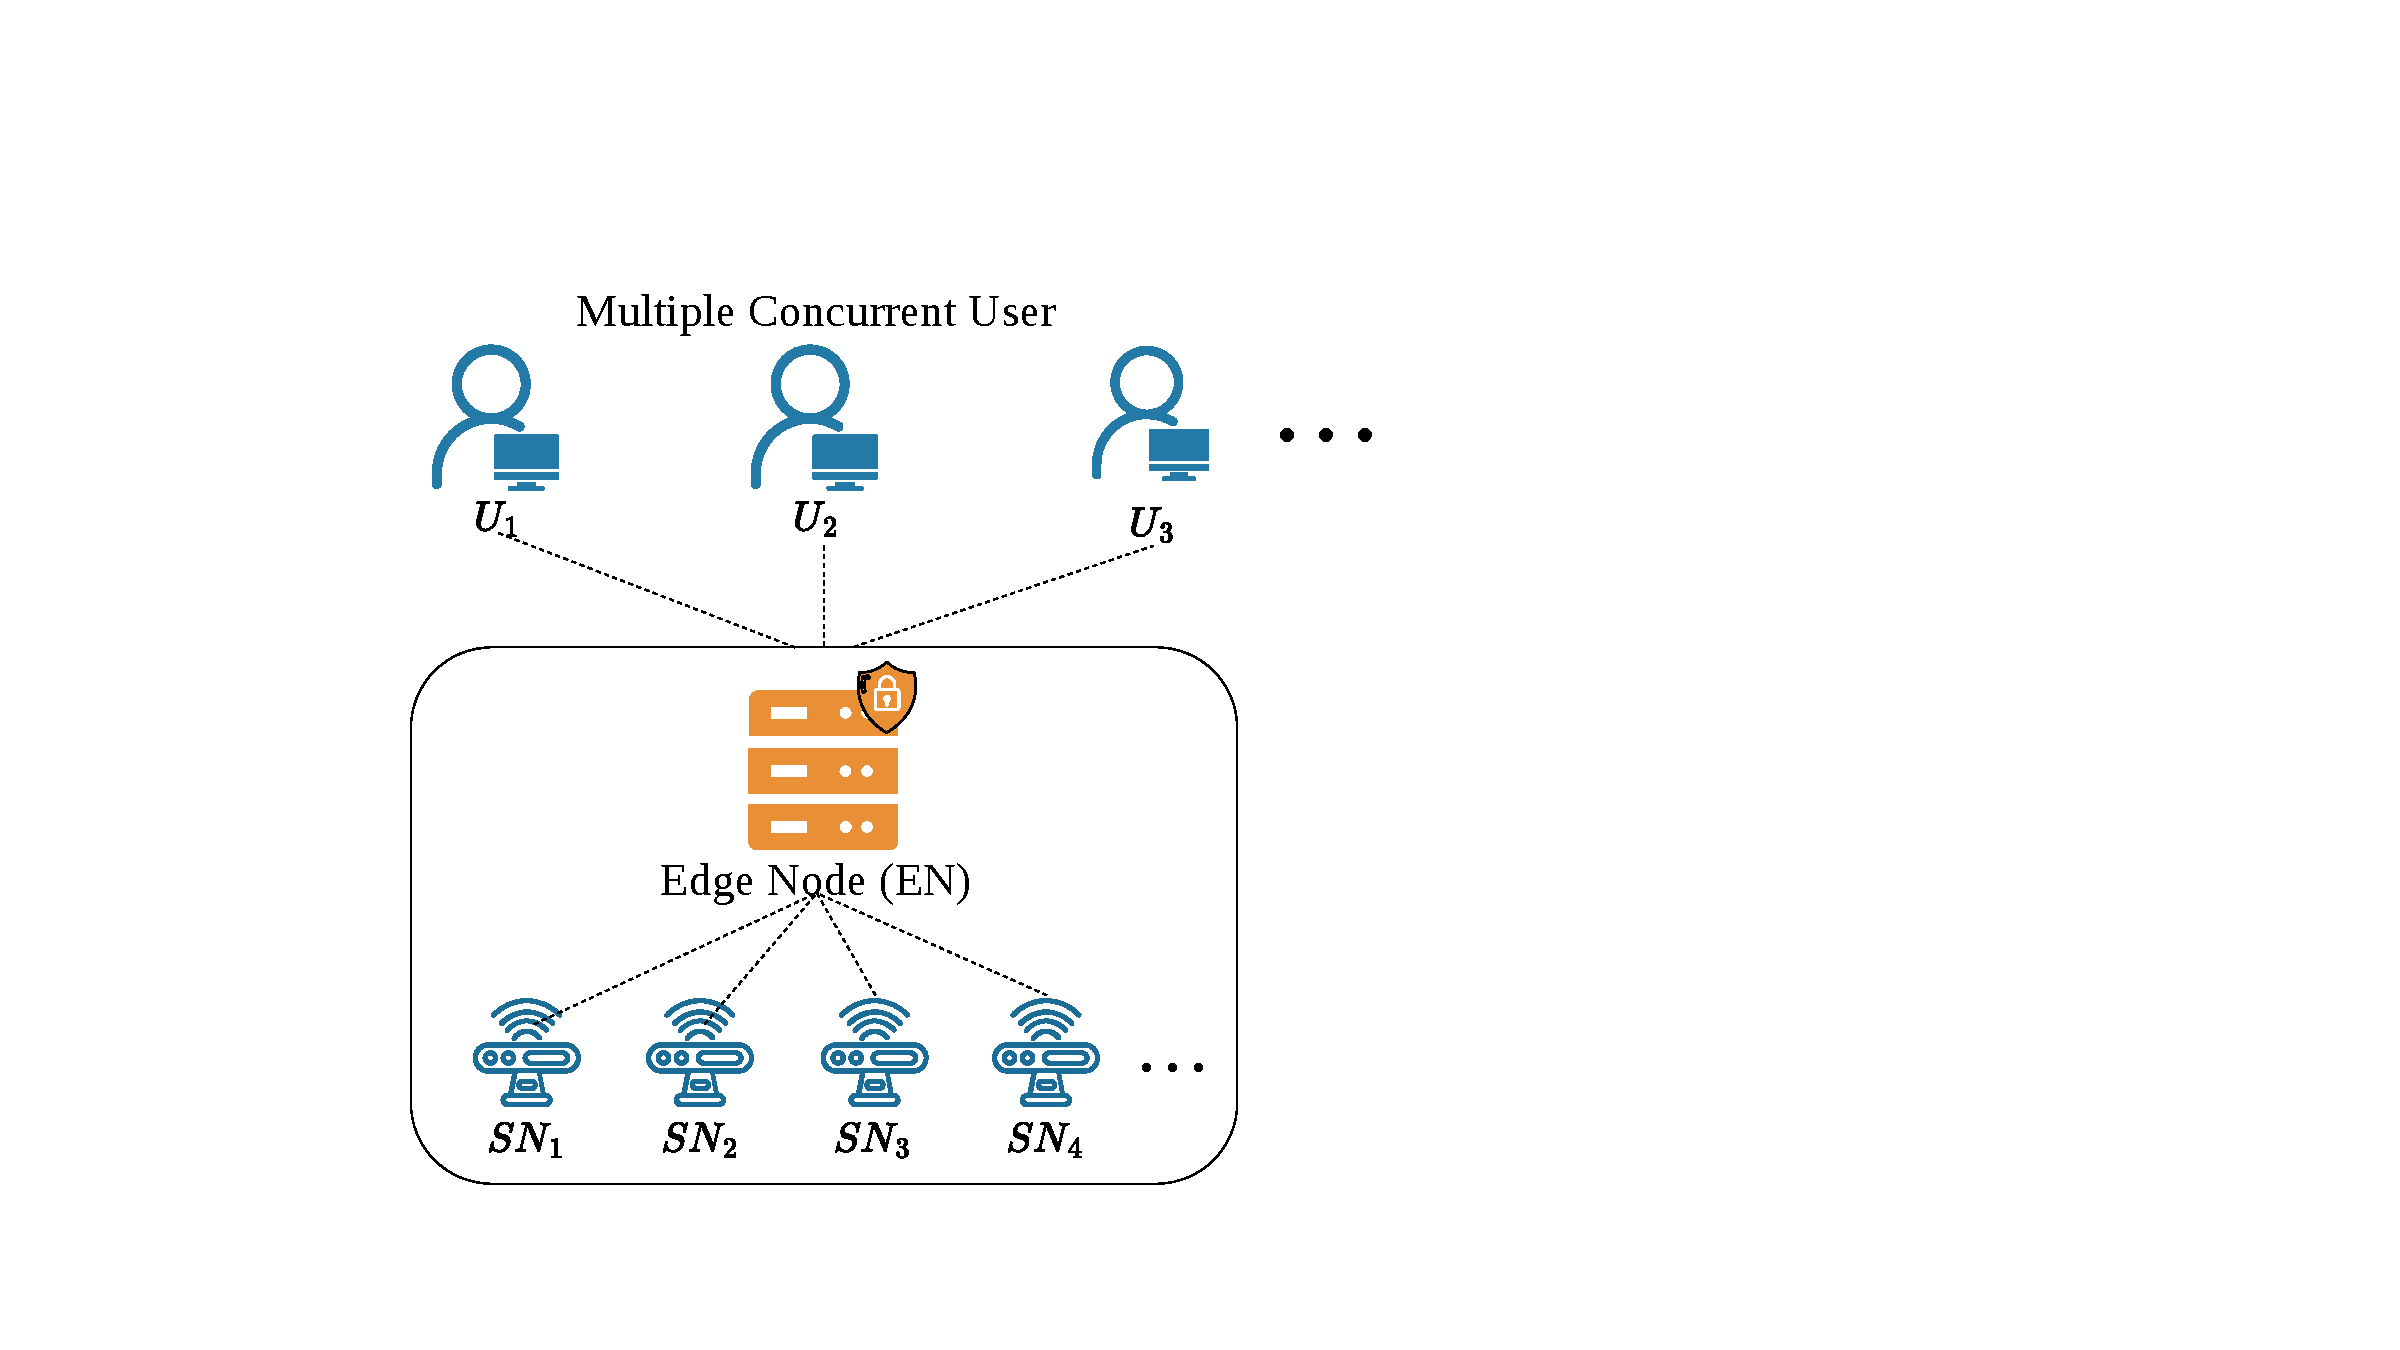
\includegraphics[width=0.4\textwidth]{netmodel.pdf}
\caption{Network model of the edge-collaborative IIoT scheme.\label{fig:netmodel}}
\end{figure}

\subsection{The Edge Node as a Pre-Inference Control Point}\label{sec:guardrail}

Figure~\ref{fig:netmodel} is usually read as a routing diagram. Under edge intelligence it is better read as a control diagram, because two distinct paths converge on $EN$ and both of them terminate at the local model rather than at a data store.

On the request path, $U$ authenticates to $EN$ and, only after \DIFdelbegin \DIFdel{$Q_1$ verifies the four credentials}\DIFdelend \DIFaddbegin \DIFadd{the four-credential transcript check succeeds}\DIFaddend , obtains a session in which it may issue a query against the sensing service and, in a deployment that hosts analytics, against the inference service exposed by the same node. An \DIFdelbegin \DIFdel{unauthenticated }\DIFdelend \DIFaddbegin \DIFadd{unauthorized }\DIFaddend request at this position is not merely an \DIFdelbegin \DIFdel{unauthorised }\DIFdelend \DIFaddbegin \DIFadd{unauthorized }\DIFaddend read: it is an \DIFdelbegin \DIFdel{unauthorised }\DIFdelend \DIFaddbegin \DIFadd{unauthorized }\DIFaddend query against a deployed model, and repeated queries from that position are the standard precondition for extraction and membership-inference attacks \cite{tramer2016stealing,shokri2017membership}. On the ingestion path, $SN$ authenticates to $EN$ under $TC_j$ before its measurements are accepted into the aggregation that feeds local processing. An \DIFdelbegin \DIFdel{unauthenticated }\DIFdelend \DIFaddbegin \DIFadd{unauthorized }\DIFaddend sensor at this position is a channel through which fabricated observations reach the model's input, which is the deployment-time analogue of data poisoning \cite{nist2025aml,carlini2024poisoning}. The protocol is agnostic to what the local pipeline computes; what it fixes is the pair of admission decisions in front of it.

The assets guarded are therefore the model-query interface, the local inference service, and the sensor-input path, together with the session key that protects the resulting user--sensor exchange. Table~\ref{tab:coverage} states which attacks against those assets this paper claims to address and which it deliberately leaves to the model-level layer, so that the security claims of Sections~\ref{sec:security} and~\ref{sec:eval} are read against a fixed boundary.

%DIF <  OPTIONAL: a control-flow figure for this subsection. fig_guardrail.tex uses
%DIF <  base TikZ only and needs no preamble change; uncomment the next line to use
%DIF <  it, and add a sentence referring to Figure~\ref{fig:guardrail} above.
%DIF <  \input{fig_guardrail}
\DIFdelbegin %DIFDELCMD < 

%DIFDELCMD < %%%
\DIFdelend \begin{table}[t]
\caption{Coverage of the authentication guardrail at an AI-enabled edge node.\label{tab:coverage}}
\begin{tabularx}{\textwidth}{Xcl}
\toprule
\textbf{Attack or exposure} & \textbf{Addressed here} & \textbf{Where}\\
\midrule
Unauthenticated access to the model-query or inference interface & Y & Sec.~\ref{sec:aka}, $Q_1$\\
Unauthenticated or spoofed sensor input entering the aggregation path & Y & Secs.~\ref{sec:registration},~\ref{sec:aka}\\
Offline attack \DIFdelbeginFL \DIFdelFL{on }\DIFdelendFL \DIFaddbeginFL \DIFaddFL{using }\DIFaddendFL a leaked verifier \DIFdelbeginFL \DIFdelFL{, including model-assisted guessing }\DIFdelendFL \DIFaddbeginFL \DIFaddFL{or recorded transcript }\DIFaddendFL & \DIFdelbeginFL \DIFdelFL{Y }\DIFdelendFL \DIFaddbeginFL \DIFaddFL{Partly }\DIFaddendFL & Secs.~\ref{sec:ceafsec},~\ref{sec:ror}\\
Exposure of up to three of the four credentials & \DIFdelbeginFL \DIFdelFL{Y}\DIFdelendFL \DIFaddbeginFL \DIFaddFL{Partly}\DIFaddendFL $^{a}$ & \DIFdelbeginFL \DIFdelFL{Secs}\DIFdelendFL \DIFaddbeginFL \DIFaddFL{Sec}\DIFaddendFL .~\ref{sec:ror}\DIFdelbeginFL \DIFdelFL{,~\ref{sec:informal}}\DIFdelendFL \\
Replay, modification, impersonation, man-in-the-middle & Y & Sec.~\DIFdelbeginFL \DIFdelFL{\ref{sec:informal}}\DIFdelendFL \DIFaddbeginFL \DIFaddFL{\ref{sec:security}}\DIFaddendFL \\
Endpoint identity exposure to a channel observer & Y$^{b}$ & Sec.~\DIFdelbeginFL \DIFdelFL{\ref{sec:informal}}\DIFdelendFL \DIFaddbeginFL \DIFaddFL{\ref{sec:security}}\DIFaddendFL \\
Loss of one authentication message (credential \DIFdelbeginFL \DIFdelFL{desynchronisation}\DIFdelendFL \DIFaddbeginFL \DIFaddFL{desynchronization}\DIFaddendFL ) & Y$^{c}$ & Sec.~\ref{sec:desync}\\
Distributed flooding of the edge node & Partly$^{d}$ & Sec.~\DIFdelbeginFL \DIFdelFL{\ref{sec:informal}}\DIFdelendFL \DIFaddbeginFL \DIFaddFL{\ref{sec:security}}\DIFaddendFL \\
\midrule
Prompt injection against a generative component & N & Sec.~\ref{sec:aisec}\\
Training-data or model poisoning after admission & N & Sec.~\ref{sec:aisec}\\
Adversarial examples at inference time & N & Sec.~\ref{sec:aisec}\\
Extraction or membership inference by an authenticated client & N$^{e}$ & Sec.~\ref{sec:aisec}\\
Detection of AI-assisted malware, ransomware, or intrusion & N & \DIFdelbeginFL \DIFdelFL{detector layer}\DIFdelendFL \DIFaddbeginFL \DIFaddFL{outside scope}\DIFaddendFL \\
Extraction of TEE-protected edge secrets & N & Sec.~\ref{sec:netmodel}\\
\bottomrule
\end{tabularx}
\DIFdelbeginFL %DIFDELCMD < \noindent{\footnotesize $^{a}$ Reduced to rate-controlled online CEAF guessing, not to full-strength security. $^{b}$ Anonymity from the channel, not from $EN$. $^{c}$ One lost message in $M_1$--$M_4$ only. $^{d}$ Mitigated by rate limits and a non-extending cooldown; not prevented. $^{e}$ The guardrail bounds \emph{who} may query, which reduces the population able to mount such attacks, but gives no protection once a client is authenticated.}
%DIFDELCMD < %%%
\DIFdelendFL \DIFaddbeginFL \noindent{\footnotesize $^{a}$ With $(SC,PW,BIO)$ exposed, a recorded $Q_1$ permits offline enumeration of the CEAF response; live attempts remain subject to deployment source/global limits, but no offline resistance is claimed. $^{b}$ Anonymity from the channel, not from $EN$. $^{c}$ The two-record window absorbs one lost $M_1$--$M_4$ message; repeated sensor-side loss invokes authenticated $M_{R1}$--$M_{R2}$ recovery, while credential update uses a separate bounded authenticated retry. $^{d}$ Source/global ingress and concurrency limits reduce processing pressure but do not prevent distributed flooding. $^{e}$ The guardrail bounds \emph{who} may query, which reduces the population able to mount such attacks, but gives no protection once a client is authenticated.}
\DIFaddendFL \end{table}

\subsection{Threat Model}\label{sec:threat}

We use the Dolev--Yao model \cite{liu2019robust,liu2021sgx,li2019twofactor}. The adversary $\advA$ may:

\begin{itemize}
\item control both public channels by eavesdropping, replaying, modifying, dropping, and injecting protocol messages, and also act as a registered malicious user;
\item compromise at most two of the password, smart card, biometric, and CEAF credentials in the general model; we additionally analyze simultaneous exposure of the password, smart card, and biometric, in which case \DIFdelbegin \DIFdel{security reduces to rate-controlled online CEAF guessing}\DIFdelend \DIFaddbegin \DIFadd{a recorded $Q_1$ permits offline CEAF enumeration and live attempts remain rate controlled. The latter is a deliberately separate stress test: it diagnoses the residual CEAF entropy after three-credential exposure and does not replace the general two-corruption ROR experiment}\DIFaddend ;
\item capture a sensor and read all of its storage; security then concerns lateral compromise of uncaptured nodes, while the captured node itself requires revocation or re-registration;
\item access edge hardware but not extract TEE-protected secrets; and
\item observe the displayed challenge and selected CEAF response for at most one successful login. This observation does not by itself expose the password, card state, or biometric; combining it with all three is full credential compromise and is outside the security claim. Two consecutive CEAF observations recover $(\mathbf{N},\mathbf{N}_S)$ and are likewise excluded; \DIFaddbegin \DIFadd{this is an environmental observation bound, not a cryptographic guarantee; }\DIFaddend and
\item automate \DIFdelbegin \DIFdel{any of the above, including with learned or generative components. Automation is treated as a change in }\DIFdelend \DIFaddbegin \DIFadd{password guessing or biometric synthesis. Automation changes }\DIFaddend the rate and per-attempt success probability\DIFdelbegin \DIFdel{of guessing and of biometric synthesis, not as a change in }\DIFdelend \DIFaddbegin \DIFadd{, not }\DIFaddend the set of values obtainable by $\advA$. \DIFdelbegin \DIFdel{In particular, offline }\DIFdelend \DIFaddbegin \DIFadd{Offline }\DIFaddend work against a password verifier or \DIFdelbegin \DIFdel{a }\DIFdelend biometric template is assumed to \DIFdelbegin \DIFdel{be as fast as }\DIFdelend \DIFaddbegin \DIFadd{proceed at }\DIFaddend the adversary's \DIFdelbegin \DIFdel{own hardware allows, and is bounded only through the credential terms of Section~\ref{sec:formal}; the }\DIFdelend \DIFaddbegin \DIFadd{hardware speed. The }\DIFaddend one-successful-login limit on CEAF observation is \DIFdelbegin \DIFdel{retained as a modelling }\DIFdelend \DIFaddbegin \DIFadd{a modeling }\DIFaddend assumption and is revisited in Section~\ref{sec:conclusions}.
\end{itemize}

The adversary is correspondingly \emph{not} assumed to attack the model behind the guardrail. Adversarial examples, poisoning of the locally hosted model, prompt injection against a generative component, and extraction or membership inference mounted from a session that has already been admitted are excluded by assumption rather than defended against; Table~\ref{tab:coverage} records the division and Section~\ref{sec:aisec} identifies the layer to which those attacks belong. A registered malicious user \DIFdelbegin \DIFdel{remains inside the model in the sense of the first bullet---it }\DIFdelend may deviate arbitrarily in the \DIFdelbegin \DIFdel{protocol---but }\DIFdelend \DIFaddbegin \DIFadd{protocol, but }\DIFaddend no claim is made about what it does with the inference service once a session is established.

\DIFdelbegin \DIFdel{For the main protocol, corruption }\DIFdelend \DIFaddbegin \DIFadd{Corruption }\DIFaddend of $R_i$, $TC_i$, $TC_j$, or $R_{EN}$ makes a \DIFaddbegin \DIFadd{main-protocol }\DIFaddend session non-fresh because \DIFdelbegin \DIFdel{those }\DIFdelend \DIFaddbegin \DIFadd{these }\DIFaddend values reconstruct transcript nonces. \DIFdelbegin \DIFdel{The PFS design sketch instead considers post-session long-term corruption after the ephemeral scalars have been erased. }\DIFdelend Hash inversion, second-preimage construction, collision finding, nonce prediction, and compromise of the secure registration channel are assumed infeasible. All claims in Section~\ref{sec:security} are scoped to these freshness and compromise conditions.

\subsection{Notation}

The notation used throughout this paper is listed in Table~\ref{tab:notation}.

\begin{table}[t]
\caption{Notation definitions.\label{tab:notation}}
\begin{tabularx}{\textwidth}{lX}
\toprule
\textbf{Symbol} & \textbf{Meaning}\\
\midrule
$U,\ EN,\ SN$ & User, edge node, sensor node\\
$LD,\ SC$ & User device and smart card\\
$SA,\ \advA$ & System administrator, adversary\\
$ID_i, ID_{SC}, ID_{SN}, ID_{EN}$ & Unique identities of $U$, $SC$, $SN$, $EN$\\
$PID_i, PID_j$ & Persistent pseudo-identities of $U$ and $SN$\\
$PID_{SN}$ & One-time pseudo-identity of $SN$\\
$PW_i,\ SK$ & User static password and session key\\
$TS,\ \Delta T,\ \sigma$ & Timestamp, acceptance window, and $160$-bit challenge seed\\
\DIFaddbeginFL \DIFaddFL{$r_R,\ C_R^{cur},\ C_R^{prev}$ }& \DIFaddFL{Resynchronization nonce and masked sensor-version identifiers}\\
\DIFaddendFL $RS,\ \mathsf{Exp}(\cdot)$ & Challenge $RS=\mathsf{Exp}(\sigma)\in\Sigma^{L}$ and its expansion function\\
$s,\ \ell,\ L$ & Segment count, segment length, challenge length $L=s\ell$\\
$\mathbf{N},\ \mathbf{N}_S$ & CEAF offset vector and step vector in $\mathbb{Z}_{26}^{s}$\\
$DPW$ & One-time CEAF response $\CT_{\mathbf{N}}(RS)$\\
\DIFdelbeginFL \DIFdelFL{$\rho,\ ctr_i$ }%DIFDELCMD < & %%%
\DIFdelFL{Consecutive-failure limit and its counter at $EN$}%DIFDELCMD < \\
%DIFDELCMD < %%%
\DIFdelendFL $\Gen(\cdot)/\Rep(\cdot)$ & Generation/reproduction algorithm of the fuzzy extractor\\
$\CT_{\mathbf{N}}(\cdot)$ & Segmented cognitive-binding primitive with offset vector $\mathbf{N}$\\
$h(\cdot),\ \cc,\ \oplus$ & Hash function, concatenation, XOR\\
\DIFaddbeginFL \DIFaddFL{$\operatorname{enc}_s,\operatorname{dec}_s$ }& \DIFaddFL{Fixed-length encoding of $\mathbb{Z}_{26}^{s}$ and its inverse on the encoding image}\\
\DIFaddFL{$T_H,\ T_F$ }& \DIFaddFL{Analytical unit costs of one hash and one fuzzy-extractor operation; values are illustrative}\\
\DIFaddendFL \bottomrule
\end{tabularx}
\end{table}

%%%%%%%%%%%%%%%%%%%%%%%%%%%%%%%%%%%%%%%%%%
\section{The Proposed Scheme}\label{sec:scheme}

The scheme has initialization, registration, login, AKA, and update phases\DIFdelbegin \DIFdel{, plus the PFS design sketch of Section~\ref{sec:pfs}}\DIFdelend . Verification is \DIFdelbegin \DIFdel{deliberately }\DIFdelend divided between two locations: $LD$ checks the password, card, and biometric, while $EN$ checks \DIFdelbegin \DIFdel{the }\DIFdelend CEAF through the first protocol authenticator. \DIFdelbegin \DIFdel{Consequently, possession of the first three credentials does not provide a local CEAF verifier , although it leaves a rate-controlled online guess}\DIFdelend \DIFaddbegin \DIFadd{The transcript binding prevents a verifier from being stored on the card, but a recorded $Q_1$ can still be tested offline after the other three credentials are exposed}\DIFaddend . Apart from fuzzy reproduction and challenge expansion, the \DIFdelbegin \DIFdel{main }\DIFdelend protocol uses hashes, XOR, nonces, and timestamps. \DIFdelbegin \DIFdel{The rotating }\DIFdelend \DIFaddbegin \DIFadd{Rotating }\DIFaddend pseudo-identities and CEAF state are maintained as version-bound two-record windows to tolerate one lost authentication message. \DIFaddbegin \DIFadd{Protocol displays are numbered $(P1),(P2),\ldots$ for implementation reference; the analytical security bounds use ordinary equation numbers (1)--(3).
}\DIFaddend 

\subsection{System Initialization Phase}

Before deployment, the system administrator $SA$ provisions each device as follows:

\begin{enumerate}
\item Install the primitive set $\{\oplus, h(\cdot), \cc\}$ on every $LD$, $EN$, and $SN$.
\item Install \DIFdelbegin \DIFdel{the challenge-expansion function }\DIFdelend $\mathsf{Exp}(\cdot)$ \DIFdelbegin \DIFdel{of }\DIFdelend \DIFaddbegin \DIFadd{from }\DIFaddend Section~\ref{sec:challenge} on every $LD$ and $EN$\DIFdelbegin \DIFdel{, the segmented cognitive-binding primitive }\DIFdelend \DIFaddbegin \DIFadd{; install }\DIFaddend $\CT_{\mathbf{N}}(\cdot)$ on every $EN$ and \DIFdelbegin \DIFdel{on every }\DIFdelend \DIFaddbegin \DIFadd{in the }\DIFaddend $LD$ display routine, and \DIFdelbegin \DIFdel{the fuzzy-extractor algorithms }\DIFdelend \DIFaddbegin \DIFadd{install }\DIFaddend $\{\Gen(\cdot),\Rep(\cdot)\}$ on every $LD$.
\item Fix the CEAF parameters \DIFdelbegin \DIFdel{$(s,\ell,\rho)$ }\DIFdelend \DIFaddbegin \DIFadd{$(s,\ell)$ }\DIFaddend and timestamp-acceptance window $\Delta T$ system-wide; this paper uses \DIFdelbegin \DIFdel{$(3,7,5)$ for the CEAF parameters. Let $\langle\cdot\rangle$ }\DIFdelend \DIFaddbegin \DIFadd{$(3,7)$. Let $\langle\cdot\rangle=\operatorname{enc}_s(\cdot)$ }\DIFaddend denote the fixed-length $160$-bit encoding of a vector in $\mathbb{Z}_{26}^{s}$\DIFaddbegin \DIFadd{, and let $\operatorname{dec}_s$ be its inverse on the encoding image. Thus $\operatorname{dec}_s$ is string decoding, not group inversion. Source/global ingress budgets are deployment parameters and are not stored in $\Lambda_i$}\DIFaddend .
\item Assign a unique identity $ID_{SC}$ to each smart card, $ID_{SN}$ to each sensor node, and $ID_{EN}$ to the edge node. Each edge domain samples one master secret $R_{EN}$ and seals it inside the TEE before any registration.
\end{enumerate}

\subsection{Registration Phase}\label{sec:registration}

Registration uses a secure channel and binds each user to a unique smart card and each sensor to the edge domain. Long-term credentials are stored in masked form, and $R_{EN}$ remains inside the TEE. The user sends the CEAF vectors to $EN$ only during registration and erases the working copies on $LD$; this placement \DIFdelbegin \DIFdel{is what }\DIFdelend prevents the card or login device from becoming a CEAF verification oracle.

\subsubsection{User Registration}

\begin{enumerate}
\item $U$ supplies its identity, password, biometric, and CEAF vectors. $LD$ reads $ID_{SC}$, samples $R_i$, obtains $TS_1$, and computes

\DIFdelbegin %DIFDELCMD < \begin{center}
%DIFDELCMD < %%%
\DIFdelend \DIFaddbegin \begin{ceq}
\DIFaddend \begin{adjustbox}{max width=\columnwidth}
$\displaystyle\begin{aligned}
(R_U, P_U) &= \Gen(BIO_i),\\
UID_i &= h(ID_i \cc PW_i),\\
HPW &= h(ID_i \cc PW_i \cc ID_{SC} \cc R_U \cc R_i),
\end{aligned}$
\end{adjustbox}
\DIFdelbegin %DIFDELCMD < \end{center}
%DIFDELCMD < %%%
\DIFdelend \DIFaddbegin \end{ceq}
\DIFaddend 

then sends the registration tuple
\DIFdelbegin %DIFDELCMD < \begin{center}
%DIFDELCMD < %%%
\DIFdelend \DIFaddbegin \begin{ceq}
\DIFaddend \begin{adjustbox}{max width=\linewidth}
$\{UID_i, ID_{SC}, HPW, R_i, \langle\mathbf{N}\rangle, \langle\mathbf{N}_S\rangle, TS_1\}$
\end{adjustbox}
\DIFdelbegin %DIFDELCMD < \end{center}
%DIFDELCMD < %%%
\DIFdelend \DIFaddbegin \end{ceq}
\DIFaddend to $EN$ over the secure channel and erases the CEAF vectors.

\item After checking $TS_1$, $EN$ uses its TEE-resident domain secret $R_{EN}$, obtains $TS_2$, and computes

\DIFdelbegin %DIFDELCMD < \begin{center}
%DIFDELCMD < %%%
\DIFdelend \DIFaddbegin \begin{ceq}
\DIFaddend \begin{adjustbox}{max width=\columnwidth}
$\displaystyle\begin{aligned}
TC_i &= h(R_{EN} \cc R_i),\\
PID_i &= h(UID_i \cc ID_{SC} \cc R_i),\\
PTC_i &= TC_i \oplus h(R_i \cc UID_i \cc HPW),\\
RPW &= h(TC_i \cc R_i),
\end{aligned}$
\end{adjustbox}
\DIFdelbegin %DIFDELCMD < \end{center}
%DIFDELCMD < %%%
\DIFdelend \DIFaddbegin \end{ceq}
\DIFaddend 

returns $\{PID_i, RPW, PTC_i, TS_2\}$ to $LD$. \DIFdelbegin \DIFdel{On the }\DIFdelend $EN$ \DIFdelbegin \DIFdel{side it }\DIFdelend then forms the masked credential state

\DIFdelbegin %DIFDELCMD < \begin{center}
%DIFDELCMD < %%%
\DIFdelend \DIFaddbegin \begin{ceq}
\DIFaddend \begin{adjustbox}{max width=\columnwidth}
$\displaystyle\begin{aligned}
PK_i &= R_i \oplus h(R_{EN} \cc ID_{EN}),\\
PN_{EN} &= \langle\mathbf{N}\rangle \oplus h(TC_i \cc R_{EN}),\\
PNS_{EN} &= \langle\mathbf{N}_S\rangle \oplus h(TC_i \cc ID_{EN} \cc R_{EN}),
\end{aligned}$
\end{adjustbox}
\DIFdelbegin %DIFDELCMD < \end{center}
%DIFDELCMD < %%%
\DIFdelend \DIFaddbegin \end{ceq}
\DIFaddend 

and stores the two-record state
\DIFdelbegin %DIFDELCMD < \begin{center}
%DIFDELCMD < %%%
\DIFdelend \DIFaddbegin \begin{ceq}
\DIFaddend \begin{adjustbox}{max width=\linewidth}
\DIFdelbegin \DIFdel{$\displaystyle\Lambda_i=\{PID_i^{cur},PID_i^{prev},PK_i,PN_{EN},PNS_{EN},ctr_i\},$
}\DIFdelend \DIFaddbegin \DIFadd{$\displaystyle\Lambda_i=\{PID_i^{cur},PID_i^{prev},PK_i,PN_{EN},PNS_{EN}\},$
}\DIFaddend \end{adjustbox}
\DIFdelbegin %DIFDELCMD < \end{center}
%DIFDELCMD < %%%
\DIFdelend \DIFaddbegin \end{ceq}
\DIFaddend with $PID_i^{cur}=PID_i^{prev}=PID_i$\DIFdelbegin \DIFdel{and $ctr_i=0$}\DIFdelend . Because $PK_i$ is masked by $R_{EN}$ rather than $PID_i$, only the rotating identifier is duplicated. The CEAF vectors remain only at $EN$\DIFaddbegin \DIFadd{; invalid authentication attempts do not modify this record}\DIFaddend .

\item After checking $TS_2$, $LD$ computes
\DIFdelbegin %DIFDELCMD < \begin{center}
%DIFDELCMD < %%%
\DIFdelend \DIFaddbegin \begin{ceq}
\DIFaddend $\displaystyle PR_i = R_i \oplus h(UID_i \cc ID_{SC} \cc R_U)$
\DIFdelbegin %DIFDELCMD < \end{center}
%DIFDELCMD < %%%
\DIFdelend \DIFaddbegin \end{ceq}
\DIFaddend and stores the five fields $PID_i$, $RPW$, $PTC_i$, $PR_i$, and $P_U$, then erases its working secrets. The provisioned public identifier $ID_{SC}$ is not counted as cryptographic state, and $SC$ stores no CEAF representation.
\end{enumerate}

\subsubsection{Sensor-Node Registration}

Sensor registration proceeds as follows.

\begin{enumerate}
\item $SN$ takes its own identity $ID_{SN}$, samples $R_j$, \DIFaddbegin \DIFadd{computes $PID_j=h(ID_{SN}\cc R_j)$ and $TC_j=h(R_j\cc ID_{SN}\cc ID_{EN})$, }\DIFaddend obtains $TS_1$, and sends $\{ID_{SN}, R_j, TS_1\}$ to $EN$. \DIFaddbegin \DIFadd{It retains $PID_j$ until the returned state is installed.
}\DIFaddend \item Upon receipt, $EN$ first checks the freshness of $TS_1$; if it has expired, $EN$ aborts. Otherwise $EN$ obtains $TS_2$ and computes

\DIFdelbegin %DIFDELCMD < \begin{center}
%DIFDELCMD < %%%
\DIFdelend \DIFaddbegin \begin{ceq}
\DIFaddend \begin{adjustbox}{max width=\columnwidth}
$\displaystyle\begin{aligned}
PID_j &= h(ID_{SN} \cc R_j),\\
TC_j &= h(R_j \cc ID_{SN} \cc ID_{EN}),\\
PK_j &= R_j \oplus h(PID_j \cc ID_{EN}),\\
PTC_j &= TC_j \oplus PID_j,
\end{aligned}$
\end{adjustbox}
\DIFdelbegin %DIFDELCMD < \end{center}
%DIFDELCMD < %%%
\DIFdelend \DIFaddbegin \end{ceq}
\DIFaddend 

returns $\{PTC_j, TS_2\}$ to $SN$, and stores the two-record state $\Lambda_j=\{PID_j^{cur}, PID_j^{prev}, PK_j\}$ indexed by $ID_{SN}$, with $PID_j^{cur}=PID_j^{prev}=PID_j$.

\item Upon receipt, $SN$ first checks the freshness of $TS_2$; if it has expired, $SN$ aborts. Otherwise $SN$ stores \DIFdelbegin \DIFdel{$\{PTC_j^{cur}, PTC_j^{prev}\}$, both initialised to }\DIFdelend \DIFaddbegin \DIFadd{$\{PID_j^{cur},PID_j^{prev},PTC_j^{cur},PTC_j^{prev}\}$, with both $PID$ entries initialized to $PID_j$ and both $PTC$ entries initialized to }\DIFaddend $PTC_j$\DIFaddbegin \DIFadd{; it then erases $R_j$ and $TC_j$}\DIFaddend .
\end{enumerate}

\subsection{User Login Phase}\label{sec:login}

The login phase separates local screening from remote authentication. $LD$ first rejects an incorrect password, card, or biometric without creating network traffic. It then \DIFdelbegin \DIFdel{only collects }\DIFdelend \DIFaddbegin \DIFadd{collects only }\DIFaddend the CEAF response; $EN$ verifies that response through $M_1$. This order limits unnecessary edge and sensor work while preserving the requirement that the fourth credential be checked against edge-only state.

\textbf{(1) Verification of the first three credentials (static password, smart card, biometric).} $U$ inserts $SC$ into $LD$, inputs $\{ID_i, PW_i\}$, and \DIFdelbegin \DIFdel{imprints }\DIFdelend \DIFaddbegin \DIFadd{provides biometric }\DIFaddend $BIO_i$. $LD$ reads the smart-card state and computes

\DIFdelbegin %DIFDELCMD < \begin{center}
%DIFDELCMD < %%%
\DIFdelend \DIFaddbegin \begin{ceq}
\DIFaddend \begin{adjustbox}{max width=\columnwidth}
$\displaystyle\begin{aligned}
UID_i &= h(ID_i \cc PW_i),\\
R_U &= \Rep(P_U, BIO_i),\\
R_i &= PR_i \oplus h(UID_i \cc ID_{SC} \cc R_U),\\
HPW &= h(ID_i \cc PW_i \cc ID_{SC} \cc R_U \cc R_i),\\
TC_i &= PTC_i \oplus h(R_i \cc UID_i \cc HPW),\\
RPW^{*} &= h(TC_i \cc R_i).
\end{aligned}$
\end{adjustbox}
\DIFdelbegin %DIFDELCMD < \end{center}
%DIFDELCMD < %%%
\DIFdelend \DIFaddbegin \end{ceq}
\DIFaddend 

If $RPW^{*}\neq RPW$, $LD$ rejects; otherwise the first three credentials pass.

\textbf{(2) CEAF collection.} $U$ selects the target sensor $ID_{SN}$ and verifies the target shown by $LD$. $LD$ then samples $\sigma$, displays the candidate columns for $RS=\mathsf{Exp}(\sigma)$, and receives $DPW$. It retains $(\sigma,RS,DPW)$ only through $M_1$ construction and does not verify $DPW$. $U$ advances the offset only after session confirmation.

\subsection{Authentication and Key Agreement Phase}\label{sec:aka}

$U$, $EN$, and $SN$ authenticate, establish $SK$ for $U$ and $SN$, and rotate credentials. $M_1$ binds the four-credential login and target sensor, $M_2$ carries the edge contribution to the selected sensor, $M_3$ returns the sensor contribution, and $M_4$ confirms both nonces to the user. \DIFdelbegin \DIFdel{Trusted }\DIFdelend \DIFaddbegin \DIFadd{Because }\DIFaddend $EN$ \DIFaddbegin \DIFadd{is trusted, it }\DIFaddend learns $X$, $Y$, and therefore $SK$ (A15); it verifies the CEAF in step~(2). The timestamps provide freshness, whereas the $Q$ values bind the reconstructed fields and prevent an adversary from changing a timestamp or masked nonce independently.

All replay and concurrency checks are atomic. Within $\Delta T$, $EN$ caches $(PID_i,Q_1,TS_1)$ for $M_1$, and $SN$ caches $(PID_j,Q_2,TS_2)$ for $M_2$. For $M_3$ and $M_4$, $EN$ and $LD$ cache $(Q_3,TS_3)$ and $(Q_4,TS_4)$, respectively. A duplicate is rejected before any state transition. $LD$ retains one outstanding local context; $EN$ and $SN$ allow at most one accepted in-flight session for the relevant user and sensor records. $M_3$ must match the sole pending sensor context at $EN$, and $M_4$ must match the outstanding context at $LD$. Reservations and replay entries expire after $\Delta T$. These bounded caches and locks are required protocol metadata but are excluded from the static cryptographic-storage comparison in Section~\ref{sec:eval}.

\textbf{(1)} $LD$ samples a fresh random number $X$, obtains a timestamp $TS_1$, and computes

\DIFdelbegin %DIFDELCMD < \begin{center}
%DIFDELCMD < %%%
\DIFdelend \DIFaddbegin \begin{ceq}
\DIFaddend \begin{adjustbox}{max width=\columnwidth}
$\displaystyle\begin{aligned}
PKS_1 &= X \oplus h(R_i \cc TC_i \cc TS_1),\\
PRS &= \sigma \oplus h(X \cc TC_i \cc TS_1),\\
PID_{SN} &= ID_{SN} \oplus h(X \cc TC_i),\\
Q_1 &= h(X \cc ID_{SN} \cc PID_i \cc RS \cc DPW \cc TS_1).
\end{aligned}$
\end{adjustbox}
\DIFdelbegin %DIFDELCMD < \end{center}
%DIFDELCMD < %%%
\DIFdelend \DIFaddbegin \end{ceq}
\DIFaddend 

$LD$ sends
\DIFdelbegin %DIFDELCMD < \begin{center}
%DIFDELCMD < %%%
\DIFdelend \DIFaddbegin \begin{ceq}
\DIFaddend $M_1=\{PID_i, PKS_1, PRS, PID_{SN}, Q_1, TS_1\}$
\DIFdelbegin %DIFDELCMD < \end{center}
%DIFDELCMD < %%%
\DIFdelend \DIFaddbegin \end{ceq}
\DIFaddend to $EN$ and erases $DPW$. $Q_1$ binds the untransmitted response, while $PRS$ masks the challenge seed.

\textbf{(2)} Upon receipt, $EN$ checks the freshness of $TS_1$ and the $M_1$ replay key; if either check fails, $EN$ aborts. Otherwise $EN$ \DIFdelbegin \DIFdel{locates the }\DIFdelend \DIFaddbegin \DIFadd{first searches for a }\DIFaddend state $\Lambda_i$ whose $PID_i^{cur}$ equals the received $PID_i$ \DIFdelbegin \DIFdel{, recording }\DIFdelend \DIFaddbegin \DIFadd{and records }\DIFaddend $v_i=cur$\DIFdelbegin \DIFdel{, and failing that the state whose $PID_i^{prev}$ equals it , recording }\DIFdelend \DIFaddbegin \DIFadd{. If no current value matches, it searches the previous values and records }\DIFaddend $v_i=prev$\DIFdelbegin \DIFdel{; if neither }\DIFdelend \DIFaddbegin \DIFadd{. If neither value }\DIFaddend matches or the record already has an in-flight session, $EN$ aborts. \DIFdelbegin \DIFdel{If the record is in a fixed-duration cooldown, }\DIFdelend \DIFaddbegin \DIFadd{Source/global ingress and concurrency controls are applied independently of $PID_i$; they may reject traffic before this step but never create a user-specific lock. }\DIFaddend $EN$ \DIFdelbegin \DIFdel{rejects the message without evaluating $Q_1$ and without extending the cooldown. Otherwise $EN$ }\DIFdelend \DIFaddbegin \DIFadd{then }\DIFaddend recovers

\DIFdelbegin %DIFDELCMD < \begin{center}
%DIFDELCMD < %%%
\DIFdelend \DIFaddbegin \begin{ceq}
\DIFaddend \begin{adjustbox}{max width=\linewidth}
\DIFdelbegin \DIFdel{%
\mbox{%DIFAUXCMD
$\displaystyle\begin{aligned}
R_i &= PK_i \oplus h(R_{EN} \cc ID_{EN}),\\
TC_i &= h(R_{EN} \cc R_i),\\
X &= PKS_1 \oplus h(R_i \cc TC_i \cc TS_1),\\
\sigma &= PRS \oplus h(X \cc TC_i \cc TS_1),\quad RS=\mathsf{Exp}(\sigma),\\
ID_{SN} &= PID_{SN} \oplus h(X \cc TC_i),\\
\mathbf{N} &= \langle PN_{EN} \oplus h(TC_i \cc R_{EN})\rangle^{-1},\\
\mathbf{N}_S &= \langle PNS_{EN} \oplus h(TC_i \cc ID_{EN} \cc R_{EN})\rangle^{-1},\\
Q_1^{*} &= h(X \cc ID_{SN} \cc PID_i \cc RS \cc \CT_{\mathbf{N}}(RS) \cc TS_1).
\end{aligned}$
}%DIFAUXCMD
}\DIFdelend \DIFaddbegin \DIFadd{%
\mbox{%DIFAUXCMD
$\displaystyle\begin{aligned}
R_i &= PK_i \oplus h(R_{EN} \cc ID_{EN}),\\
TC_i &= h(R_{EN} \cc R_i),\\
X &= PKS_1 \oplus h(R_i \cc TC_i \cc TS_1),\\
\sigma &= PRS \oplus h(X \cc TC_i \cc TS_1),\quad RS=\mathsf{Exp}(\sigma),\\
ID_{SN} &= PID_{SN} \oplus h(X \cc TC_i),\\
\mathbf{N} &= \operatorname{dec}_s\bigl(PN_{EN} \oplus h(TC_i \cc R_{EN})\bigr),\\
\mathbf{N}_S &= \operatorname{dec}_s\bigl(PNS_{EN} \oplus h(TC_i \cc ID_{EN} \cc R_{EN})\bigr),\\
Q_1^{*} &= h(X \cc ID_{SN} \cc PID_i \cc RS \cc \CT_{\mathbf{N}}(RS) \cc TS_1).
\end{aligned}$
}%DIFAUXCMD
}\DIFaddend \end{adjustbox}
\DIFdelbegin %DIFDELCMD < \end{center}
%DIFDELCMD < %%%
\DIFdelend \DIFaddbegin \end{ceq}
\DIFaddend 

If $Q_1$ fails and $v_i=prev$, $EN$ retries once with $\mathbf{N}^{-}=\mathbf{N}-\mathbf{N}_S\bmod26$; it never tries $\mathbf{N}^{-}$ for $PID_i^{cur}$. A match adopts the preceding offset. Any other mismatch \DIFdelbegin \DIFdel{increments $ctr_i$ and aborts . At $\rho$, a non-extending fixed cooldown begins; success resets $ctr_i$. After success}\DIFdelend \DIFaddbegin \DIFadd{aborts without changing $\Lambda_i$ or any user-specific availability state. After a valid $Q_1$}\DIFaddend , $EN$ atomically inserts the $M_1$ replay key and reserves the user record. Acceptance jointly verifies the four credentials. $EN$ then retrieves $\Lambda_j$; if its sensor record is busy, $EN$ releases the user reservation and aborts. Otherwise it reserves that record, uses $PID_j^{cur}$, obtains $TS_2$, and computes

\DIFdelbegin %DIFDELCMD < \begin{center}
%DIFDELCMD < %%%
\DIFdelend \DIFaddbegin \begin{ceq}
\DIFaddend \begin{adjustbox}{max width=\columnwidth}
$\displaystyle\begin{aligned}
R_j &= PK_j \oplus h(PID_j \cc ID_{EN}),\\
TC_j &= h(R_j \cc ID_{SN} \cc ID_{EN}),\\
PKS_2 &= X \oplus h(TC_j \cc TS_2),\\
Q_2 &= h(X \cc PID_j \cc TS_2),
\end{aligned}$
\end{adjustbox}
\DIFdelbegin %DIFDELCMD < \end{center}
%DIFDELCMD < %%%
\DIFdelend \DIFaddbegin \end{ceq}
\DIFaddend 

and sends $M_2=\{PID_j, PKS_2, Q_2, TS_2\}$ to the $SN$ designated by $ID_{SN}$.

\textbf{(3)} After checking $TS_2$, the $M_2$ replay key, and the absence of another in-flight session, $SN$ \DIFdelbegin \DIFdel{recovers $TC_j=PTC_j^{cur}\oplus PID_j$ }\DIFdelend \DIFaddbegin \DIFadd{first matches the received $PID_j$ against the stored current/previous pair. If neither identifier matches, it invokes the authenticated resynchronization of Section~\ref{sec:resync} and does not process $M_2$. Otherwise, with $v_j\in\{cur,prev\}$ denoting the matching version, $SN$ recovers $TC_j=PTC_j^{v_j}\oplus PID_j$ }\DIFaddend and $X$, then verifies $Q_2$. \DIFdelbegin \DIFdel{On failure it retries once with $PTC_j^{prev}$; if both checks fail}\DIFdelend \DIFaddbegin \DIFadd{If the check fails}\DIFaddend , it aborts \DIFaddbegin \DIFadd{without changing state}\DIFaddend . On success it atomically inserts the replay key, reserves the record, obtains $TS_3$, samples $Y$, derives $SK=h(X\cc Y)$, and computes

\DIFdelbegin %DIFDELCMD < \begin{center}
%DIFDELCMD < %%%
\DIFdelend \DIFaddbegin \begin{ceq}
\DIFaddend \begin{adjustbox}{max width=\columnwidth}
$\displaystyle\begin{aligned}
PKS_3 &= Y \oplus h(TC_j \cc X \cc TS_3),\\
Q_3 &= h(X \cc Y \cc TS_3),
\end{aligned}$
\end{adjustbox}
\DIFdelbegin %DIFDELCMD < \end{center}
%DIFDELCMD < %%%
\DIFdelend \DIFaddbegin \end{ceq}
\DIFaddend 

then sends
\DIFdelbegin %DIFDELCMD < \begin{center}
%DIFDELCMD < %%%
\DIFdelend \DIFaddbegin \begin{ceq}
\DIFaddend $M_3=\{PKS_3,Q_3,TS_3\}$
\DIFdelbegin %DIFDELCMD < \end{center}
%DIFDELCMD < %%%
\DIFdel{and shifts $(PTC_j^{cur},PTC_j^{prev})$ after deriving }\DIFdelend \DIFaddbegin \end{ceq}
\DIFadd{and derives }\DIFaddend $PID_j^{*}=PID_j\oplus h(Y\cc TS_3)$ and $PTC_j^{*}=TC_j\oplus PID_j^{*}$. It \DIFaddbegin \DIFadd{atomically shifts the sensor state to $(PID_j^{*},PID_j,PTC_j^{*},PTC_j)$, }\DIFaddend then releases its \DIFdelbegin \DIFdel{in-flight }\DIFdelend reservation while retaining the replay entry for $\Delta T$.

\textbf{(4)} After checking $TS_3$, matching $M_3$ to the pending sensor context, and rejecting a cached $M_3$ key, $EN$ recovers $Y$ and verifies $Q_3$. It then atomically inserts the replay key, obtains $TS_4$, and computes

\DIFdelbegin %DIFDELCMD < \begin{center}
%DIFDELCMD < %%%
\DIFdelend \DIFaddbegin \begin{ceq}
\DIFaddend \begin{adjustbox}{max width=\columnwidth}
$\displaystyle\begin{aligned}
PKS_4 &= Y \oplus h(R_i \cc TC_i \cc X \cc TS_4),\\
Q_4 &= h(X \cc Y \cc TS_4),
\end{aligned}$
\end{adjustbox}
\DIFdelbegin %DIFDELCMD < \end{center}
%DIFDELCMD < %%%
\DIFdelend \DIFaddbegin \end{ceq}
\DIFaddend 

and sends $M_4=\{PKS_4, Q_4, TS_4\}$ to the $LD$ held by $U$. $EN$ then advances both credential states, keeping the value it has just used as the previous entry:

\DIFdelbegin %DIFDELCMD < \begin{center}
%DIFDELCMD < %%%
\DIFdelend \DIFaddbegin \begin{ceq}
\DIFaddend \begin{adjustbox}{max width=\columnwidth}
$\displaystyle\begin{aligned}
PID_j^{*} &= PID_j \oplus h(Y \cc TS_3),\quad PK_j^{*} = R_j \oplus h(PID_j^{*} \cc ID_{EN}),\\
PID_i^{*} &= PID_i \oplus h(X \cc TS_4),\quad \mathbf{N}^{*}=\mathbf{N}+\mathbf{N}_S \bmod 26,\\
PN_{EN}^{*} &= \langle\mathbf{N}^{*}\rangle \oplus h(TC_i \cc R_{EN}),
\end{aligned}$
\end{adjustbox}
\DIFdelbegin %DIFDELCMD < \end{center}
%DIFDELCMD < %%%
\DIFdelend \DIFaddbegin \end{ceq}
\DIFaddend 

\DIFdelbegin %DIFDELCMD < \begin{center}
%DIFDELCMD < %%%
\DIFdelend \DIFaddbegin \begin{ceq}
\DIFaddend \begin{adjustbox}{max width=\columnwidth}
$\displaystyle\begin{aligned}
\{PID_j^{prev}, PID_j^{cur}, PK_j\} &\leftarrow \{PID_j, PID_j^{*}, PK_j^{*}\},\\
\{PID_i^{prev}, PID_i^{cur}, PN_{EN}\} &\leftarrow \{PID_i, PID_i^{*}, PN_{EN}^{*}\}.
\end{aligned}$
\end{adjustbox}
\DIFdelbegin %DIFDELCMD < \end{center}
%DIFDELCMD < %%%
\DIFdelend \DIFaddbegin \end{ceq}
\DIFaddend 

Here $PID_i$ and $PID_j$ are the values used in this round; $PK_i$ and $PNS_{EN}$ remain unchanged. After the atomic commit, $EN$ releases both in-flight reservations while retaining the replay entries until they expire.

\textbf{(5)} After checking $TS_4$, matching the sole outstanding context, and rejecting a cached $M_4$ key, $LD$ recovers $Y$, derives $SK$, and verifies $Q_4$. It then atomically caches the key, stores $PID_i^{*}=PID_i\oplus h(X\cc TS_4)$, consumes the outstanding context, and signals success, after which $U$ advances $\mathbf{N}$. If $M_4$ is lost, $U$ retains the old state and step~(2) absorbs the next login.

\DIFdelbegin %DIFDELCMD < \subsubsection{Two-record state and the desynchronisation invariant}%%%
\DIFdelend \DIFaddbegin \subsubsection{Two-record state and the desynchronization invariant}\DIFaddend \label{sec:desync}

$SN$ commits when it sends $M_3$, $EN$ when it sends $M_4$, and $U$ after verifying $M_4$. \DIFdelbegin \DIFdel{Dropping }\DIFdelend \DIFaddbegin \DIFadd{A single lost }\DIFaddend $M_3$ or $M_4$ therefore leaves adjacent principals \DIFaddbegin \DIFadd{at most }\DIFaddend one round apart\DIFdelbegin \DIFdel{and, without recovery }\DIFdelend , \DIFdelbegin \DIFdel{causes permanent credential desynchronisation}\DIFdelend \DIFaddbegin \DIFadd{which the two-record window absorbs. If repeated loss moves $SN$ beyond the identifiers retained by $EN$, the normal exchange stops and the authenticated recovery below is invoked; no unauthenticated rollback is allowed. The invariant protects state consistency, not availability under sustained loss: recovery still depends on delivery of the authenticated resynchronization exchange}\DIFaddend .

Each rotating value is therefore held as a version-bound $(cur,prev)$ pair:

\DIFdelbegin %DIFDELCMD < \begin{center}
%DIFDELCMD < %%%
\DIFdelend \DIFaddbegin \begin{ceq}
\DIFaddend \begin{adjustbox}{max width=\columnwidth}
\DIFdelbegin \DIFdel{%
\mbox{%DIFAUXCMD
$\displaystyle\begin{aligned}
EN&: (PID_i^{cur},\mathbf{N}),\ (PID_i^{prev},\mathbf{N}-\mathbf{N}_S),\ (PID_j^{cur},PID_j^{prev}),\\
SN&: (PTC_j^{cur},PTC_j^{prev}).
\end{aligned}$
}%DIFAUXCMD
}\DIFdelend \DIFaddbegin \DIFadd{%
\mbox{%DIFAUXCMD
$\displaystyle\begin{aligned}
EN&: (PID_i^{cur},\mathbf{N}),\ (PID_i^{prev},\mathbf{N}-\mathbf{N}_S),\ (PID_j^{cur},PID_j^{prev}),\\
SN&: (PID_j^{cur},PID_j^{prev},PTC_j^{cur},PTC_j^{prev}).
\end{aligned}$
}%DIFAUXCMD
}\DIFaddend \end{adjustbox}
\DIFdelbegin %DIFDELCMD < \end{center}
%DIFDELCMD < %%%
\DIFdelend \DIFaddbegin \end{ceq}
\DIFaddend 

$\mathbf{N}^{-}$ is recomputed from $(\mathbf{N},\mathbf{N}_S)$, avoiding another stored copy. A current $PID_i$ is verified only with $\mathbf{N}$, whereas $\mathbf{N}^{-}$ is available only after a previous-$PID_i$ match. Thus identifiers and CEAF offsets cannot be mixed across versions\DIFaddbegin \DIFadd{: a current identifier is never tested with the previous offset, and a previous identifier is never promoted to the current version without the adjacent-state commit}\DIFaddend . A previous-value match is accepted only for the immediately adjacent state and is followed by the normal commit rule. Together with the replay cache and single-session reservation, this one-round window recovers one lost $M_1$--$M_4$ without accepting a duplicate transcript. \DIFdelbegin \DIFdel{It }\DIFdelend \DIFaddbegin \DIFadd{Repeated sensor-side loss is handled only by the authenticated resynchronization below; credential update remains separate.
}

\subsubsection{Authenticated sensor resynchronization}\label{sec:resync}
\begingroup\small

\DIFadd{If $SN$ receives an $M_2$ whose $PID_j$ matches neither stored identifier, it derives $TC_j=PTC_j^{cur}\oplus PID_j^{cur}$, samples fresh $(r_R,TS_R)$, and computes
}

\begin{ceq}
\begin{adjustbox}{max width=\columnwidth}
\DIFadd{%
\mbox{%DIFAUXCMD
$\displaystyle\begin{aligned}
C_R^{cur} &= PID_j^{cur}\oplus h(TC_j\cc r_R\cc1),\\
C_R^{prev} &= PID_j^{prev}\oplus h(TC_j\cc r_R\cc2),\\
Q_R^{(1)} &= h(TC_j\cc C_R^{cur}\cc C_R^{prev}\cc r_R\cc TS_R\cc\mathrm{r1}),
\end{aligned}$
}%DIFAUXCMD
}\end{adjustbox}
\end{ceq}

\DIFadd{It sends $M_{R1}=\{C_R^{cur},C_R^{prev},r_R,Q_R^{(1)},TS_R\}$ and waits without changing state. $EN$ recovers $R_j$ from $(PID_j^{cur},PK_j)$, derives $TC_j$, checks freshness, replay, and $Q_R^{(1)}$, then cancels the stale $M_2$ context and releases its reservations. It recomputes $PK_j^{*}=R_j\oplus h(C_R^{cur}\cc ID_{EN})$, installs $(PID_j^{prev},PID_j^{cur},PK_j)=(C_R^{prev},C_R^{cur},PK_j^{*})$, and returns
}

\begin{ceq}
\begin{adjustbox}{max width=\columnwidth}
\DIFadd{$\displaystyle Q_R^{(2)}=h(TC_j\cc C_R^{cur}\cc C_R^{prev}\cc r_R\cc TS_R\cc\mathrm{r2}),\qquad
M_{R2}=\{r_R,Q_R^{(2)},TS_R\}.$
}\end{adjustbox}
\end{ceq}

\DIFadd{$SN$ accepts $M_{R2}$ only for its outstanding $r_R$ and a valid $Q_R^{(2)}$. It then installs the four recovered fields
$(C_R^{cur},C_R^{prev},TC_j\oplus C_R^{cur},TC_j\oplus C_R^{prev})$ and clears the request. If the acknowledgement is lost, it retransmits the same $M_{R1}$ within $\Delta T$ and $EN$ returns the cached acknowledgement without another state transition. This idempotent exchange repairs repeated sensor-side loss when the two endpoints can still exchange authenticated messages; it is excluded from the normal-session cost and }\DIFaddend does not claim \DIFdelbegin \DIFdel{arbitrary rollback tolerance and excludes credential update}\DIFdelend \DIFaddbegin \DIFadd{availability against distributed flooding or a permanently partitioned link}\DIFaddend .

\DIFaddbegin \endgroup

\DIFaddend \subsection{Credential Update Phase}\label{sec:update}

Password and biometric updates are card-local because they only change the masks used to recover $R_i$ and $TC_i$. Changing the edge-held CEAF vectors requires the protected exchange below. The update is executed only after a complete AKA run so that $LD$ and $EN$ can protect the new vectors with a fresh update key rather than with the user's low-entropy credentials.
The replay-cache and single-pending-context rules of Section~\ref{sec:aka} also apply to $M_5$ and $M_6$ within $\Delta T$. The update replay keys are $(Q_5,TS_5)$ at $EN$ and $(Q_6,TS_6)$ at $LD$. \DIFaddbegin \DIFadd{$LD$ keeps the pending update until a valid $M_6$ is received and retransmits the same $M_5$ after a timeout; $EN$ caches the accepted update and its $M_6$ for this retry window and resends it without a second state transition. Thus, one lost $M_6$ is recovered by an authenticated retry rather than by re-registration.
}\DIFaddend 

\begin{enumerate}
\item $LD$ completes Sections~\ref{sec:login}--\ref{sec:aka}; $U$ and $EN$ set $SK_{UE}=h(TC_i\cc X\cc Y)$.

\item $U$ selects any subset of a new password, biometric, CEAF vector, and CEAF step vector. An unchanged starred value equals its current value. For a password-only update, $(R_U^{*},P_U^{*})=(R_U,P_U)$; for a biometric-only update, $PW_i^{*}=PW_i$. If only one CEAF vector changes, the other starred vector equals its current value.

\item If the biometric changes, $LD$ obtains $(R_U^{*},P_U^{*})=\Gen(BIO_i^{*})$; otherwise it reuses $(R_U,P_U)$. It then recomputes the card-local values

\DIFdelbegin %DIFDELCMD < \begin{center}
%DIFDELCMD < %%%
\DIFdelend \DIFaddbegin \begin{ceq}
\DIFaddend \begin{adjustbox}{max width=\linewidth}
$\displaystyle\begin{aligned}
UID_i^{*} &= h(ID_i \cc PW_i^{*}),\\
HPW^{*} &= h(ID_i \cc PW_i^{*} \cc ID_{SC} \cc R_U^{*} \cc R_i),\\
PTC_i^{*} &= TC_i \oplus h(R_i \cc UID_i^{*} \cc HPW^{*}),\\
PR_i^{*} &= R_i \oplus h(UID_i^{*} \cc ID_{SC} \cc R_U^{*}),
\end{aligned}$
\end{adjustbox}
\DIFdelbegin %DIFDELCMD < \end{center}
%DIFDELCMD < %%%
\DIFdelend \DIFaddbegin \end{ceq}
\DIFaddend 

If neither CEAF vector changes, $LD$ atomically commits the five card fields, using $PTC_i^{*}$, $PR_i^{*}$, and $P_U^{*}$, and erases the working values. The update then ends without contacting $EN$. If either CEAF vector changes, $LD$ obtains $TS_5$ and computes

\DIFdelbegin %DIFDELCMD < \begin{center}
%DIFDELCMD < %%%
\DIFdelend \DIFaddbegin \begin{ceq}
\DIFaddend \begin{adjustbox}{max width=\columnwidth}
$\displaystyle\begin{aligned}
C_1 &= \langle\mathbf{N}^{*}\rangle \oplus h(SK_{UE} \cc 1 \cc TS_5),\\
C_2 &= \langle\mathbf{N}_S^{*}\rangle \oplus h(SK_{UE} \cc 2 \cc TS_5),\\
Q_5 &= h(SK_{UE} \cc \langle\mathbf{N}^{*}\rangle \cc \langle\mathbf{N}_S^{*}\rangle \cc TS_5),
\end{aligned}$
\end{adjustbox}
\DIFdelbegin %DIFDELCMD < \end{center}
%DIFDELCMD < %%%
\DIFdelend \DIFaddbegin \end{ceq}
\DIFaddend 

sending $M_5=\{C_1, C_2, Q_5, TS_5\}$ to $EN$.

\item \DIFdelbegin \DIFdel{After }\DIFdelend \DIFaddbegin \DIFadd{Upon receiving $M_5$, $EN$ first checks its pending-update cache. If $(Q_5,TS_5)$ matches an accepted update still within the retry window, it retransmits the cached $M_6$ and makes no state change. Otherwise, after }\DIFaddend checking $TS_5$ and \DIFdelbegin \DIFdel{its }\DIFdelend \DIFaddbegin \DIFadd{the }\DIFaddend replay key, $EN$ recovers
\DIFdelbegin %DIFDELCMD < \begin{center}
%DIFDELCMD < %%%
\DIFdelend \DIFaddbegin \begin{ceq}
\DIFaddend \begin{adjustbox}{max width=\columnwidth}
$\displaystyle\begin{aligned}
\langle\mathbf{N}^{*}\rangle &= C_1 \oplus h(SK_{UE} \cc 1 \cc TS_5),\\
\langle\mathbf{N}_S^{*}\rangle &= C_2 \oplus h(SK_{UE} \cc 2 \cc TS_5).
\end{aligned}$
\end{adjustbox}
\DIFdelbegin %DIFDELCMD < \end{center}
%DIFDELCMD < %%%
\DIFdelend \DIFaddbegin \end{ceq}
\DIFaddend It verifies $Q_5$, obtains $TS_6$, and computes
\DIFdelbegin %DIFDELCMD < \begin{center}
%DIFDELCMD < %%%
\DIFdelend \DIFaddbegin \begin{ceq}
\DIFaddend \begin{adjustbox}{max width=\columnwidth}
$\displaystyle\begin{aligned}
PN_{EN}^{*} &= \langle\mathbf{N}^{*}\rangle \oplus h(TC_i \cc R_{EN}),\\
PNS_{EN}^{*} &= \langle\mathbf{N}_S^{*}\rangle \oplus h(TC_i \cc ID_{EN} \cc R_{EN}),\\
Q_6 &= h(SK_{UE}\cc\langle\mathbf{N}^{*}\rangle\cc\langle\mathbf{N}_S^{*}\rangle\cc TS_6).
\end{aligned}$
\end{adjustbox}
\DIFdelbegin %DIFDELCMD < \end{center}
%DIFDELCMD < %%%
\DIFdelend \DIFaddbegin \end{ceq}
\DIFaddend $EN$ atomically stores the two starred masks, \DIFdelbegin \DIFdel{resets $ctr_i$, }\DIFdelend caches the accepted update \DIFaddbegin \DIFadd{and $M_6$}\DIFaddend , and returns $M_6=\{Q_6,TS_6\}$. \DIFaddbegin \DIFadd{It never applies an accepted update twice, and no failed $M_1$ attempt can alter this update state.
}\DIFaddend 

\item After checking $TS_6$ and verifying \DIFdelbegin \DIFdel{and caching }\DIFdelend $M_6$ against both starred CEAF vectors, $LD$ commits any new card values and $U$ memorizes the new CEAF pair. \DIFdelbegin \DIFdel{Otherwise both retain their }\DIFdelend \DIFaddbegin \DIFadd{Until this check succeeds, the }\DIFaddend old local values \DIFdelbegin \DIFdel{. Because $EN$ may already have committed, loss of }\DIFdelend \DIFaddbegin \DIFadd{are retained. If }\DIFaddend $M_6$ \DIFdelbegin \DIFdel{can require authenticated recovery or re-registration; A14 therefore covers only $M_1$--$M_4$. }\DIFdelend \DIFaddbegin \DIFadd{is lost, $LD$ retransmits the unchanged $M_5$ within $\Delta T$; the cached response above is returned and the update is committed only once. If all retries expire, $LD$ reports an incomplete update and retains its old local values; loss-atomicity is not claimed outside this bounded retry window.
}\DIFaddend \end{enumerate}

\DIFdelbegin %DIFDELCMD < \subsection{A Design Sketch for Perfect Forward Secrecy}\label{sec:pfs}
%DIFDELCMD < 

%DIFDELCMD < %%%
\DIFdel{The main protocol lacks PFS because later long-term compromise recovers transcript nonces and past keys. It also gives $EN$ visibility of the user--sensor key. The following design sketch shows how an authenticated ephemeral DH exchange could address both limitations while preserving the four-message structure; it is not presented as a fully specified or independently verified protocol. }%DIFDELCMD < 

%DIFDELCMD < %%%
\DIFdel{Let $P$ generate a prime-order group where CDH is hard. $LD$ sends $A=xP$ in }\DIFdelend %DIF > %%%%%%%%%%%%%%%%%%%%%%%%%%%%%%%%%%%%%%%%%
\DIFaddbegin \subsection{Implementation-Oriented Message Summary}
\DIFadd{The main exchange can be implemented from the following compact summary; a failed verification leaves the corresponding state unchanged. }\DIFaddend $M_1$ \DIFdelbegin \DIFdel{and binds it into }\DIFdelend \DIFaddbegin \DIFadd{($LD\rightarrow EN$) binds the four credentials, challenge, target sensor, and nonce in }\DIFaddend $Q_1$; $EN$ \DIFdelbegin \DIFdel{relays and binds $A$ in $M_2$. After validating $A$, }\DIFdelend \DIFaddbegin \DIFadd{verifies CEAF and reserves the user record. $M_2$ ($EN\rightarrow SN$) carries the masked edge contribution and $Q_2$; }\DIFaddend $SN$ \DIFdelbegin \DIFdel{sends $B=yP$ in }\DIFdelend \DIFaddbegin \DIFadd{verifies the sensor context and derives its session contribution. }\DIFaddend $M_3$ \DIFdelbegin \DIFdel{, computes $K=yA$, and sets $SK=h(X\cc Y\cc K_x\cc A\cc B)$. $Q_3$ and $Q_4$ bind $(A,B)$, while }\DIFdelend \DIFaddbegin \DIFadd{($SN\rightarrow EN$) returns the sensor contribution and $Q_3$; $SN$ shifts its two-record state after sending, while $EN$ verifies the pending context. }\DIFaddend $M_4$ \DIFdelbegin \DIFdel{relays $B$. }\DIFdelend \DIFaddbegin \DIFadd{($EN\rightarrow LD$) confirms both nonces with $Q_4$; }\DIFaddend $LD$ \DIFdelbegin \DIFdel{validates $B$, computes $K=xB$, and derives the same key. Invalid or substituted points are rejected by validation or tag failure.
}%DIFDELCMD < 

%DIFDELCMD < %%%
\DIFdel{Under honest execution, validation of both points, and erasure of $(x,y)$, CDH prevents recovery of $K$ from later long-term compromise. Binding both public points to the authenticators is necessary: relaying an unbound point would permit substitution without breaking the hash tags. Against an honest-but-curious }\DIFdelend \DIFaddbegin \DIFadd{verifies the session and commits its local identifier, while }\DIFaddend $EN$ \DIFdelbegin \DIFdel{that follows the relay procedure, the construction also hides $SK$ because $EN$ sees $A$ and $B$ but not $xyP$. A malicious intermediary is outside the trusted-edge model. The sketch adds four point multiplications and one $320$-bit point to each message (Section~\ref{sec:eval}) ; full message equations, point-validation costs, and a complete authenticated-key-exchange proof remain future work}\DIFdelend \DIFaddbegin \DIFadd{commits the adjacent records. Optional $M_5$ ($LD\rightarrow EN$) and $M_6$ ($EN\rightarrow LD$) update the CEAF vectors under $SK_{UE}$; the cached $M_6$ recovers one lost update acknowledgement without a second state transition}\DIFaddend .

%DIF < %%%%%%%%%%%%%%%%%%%%%%%%%%%%%%%%%%%%%%%%%
\section{Security Analysis}\label{sec:security}

\DIFdelbegin \DIFdel{We analyze authentication and key secrecy at three complementary levels. BAN-style correspondences check which principal can be associated with each accepted message, a }\DIFdelend \DIFaddbegin \DIFadd{The }\DIFaddend Real-or-Random (ROR) reduction bounds transcript and \DIFdelbegin \DIFdel{guessing }\DIFdelend \DIFaddbegin \DIFadd{credential-guessing }\DIFaddend attacks, and the informal audit connects those results to \DIFdelbegin \DIFdel{the properties in }\DIFdelend Table~\ref{tab:security}. \DIFdelbegin \DIFdel{These arguments }\DIFdelend \DIFaddbegin \DIFadd{The claims }\DIFaddend are conditioned on the threat model and freshness rules of Section~\ref{sec:threat}\DIFdelbegin \DIFdel{. In }\DIFdelend \DIFaddbegin \DIFadd{; in }\DIFaddend particular, the main protocol claims neither PFS nor key opacity from $EN$.

\subsection{Formal Security Analysis}\label{sec:formal}

\DIFdelbegin \DIFdel{BAN notation \cite{burrows,li2015enhancement} audits message origin and freshness; ROR handles guessing and key secrecy. We use BAN terminology only for correspondence reasoning and do not treat belief derivation as a proof of secrecy. The separation is important because the edge and sensor share some effective authenticators, making principal attribution weaker than simple tag verification might suggest.
}%DIFDELCMD < 

%DIFDELCMD < \subsubsection{BAN-Style Authentication Correspondences}
%DIFDELCMD < 

%DIFDELCMD < %%%
\DIFdel{Let $\operatorname{Auth}_K(Z)$ denote a hash authenticator reproducible only with effective secret $K$. We use only message-meaning and nonce-verification:
}%DIFDELCMD < \begin{center}
%DIFDELCMD < \begin{adjustbox}{max width=\columnwidth}
%DIFDELCMD < %%%
\DIFdel{$\displaystyle
 \frac{P\bel \shk{P}{K}{Q},\ P\sees\operatorname{Auth}_{K}(Z)}{P\bel Q\said Z},\qquad
 \frac{P\bel\fresh{Z},\ P\bel Q\said Z}{P\bel Q\bel Z}.$
}%DIFDELCMD < \end{adjustbox}
%DIFDELCMD < \end{center}
%DIFDELCMD < 

%DIFDELCMD < %%%
\DIFdel{The idealized authenticators below retain every hashed field. $K_{UE}$ denotes the effective collection of uncompromised values needed to reconstruct $Q_1$, including the edge-held CEAF state; it is not an additional protocol key.
}%DIFDELCMD < \begin{center}
%DIFDELCMD < \begin{adjustbox}{max width=\columnwidth}
%DIFDELCMD < %%%
\DIFdel{%
\mbox{%DIFAUXCMD
$\displaystyle\begin{aligned}
M_1 &: \operatorname{Auth}_{K_{UE}}(X,PID_i,PID_{SN},RS,DPW,TS_1),\\
M_2 &: \operatorname{Auth}_{TC_j}(X,PID_j,TS_2),\\
M_3 &: \operatorname{Auth}_{TC_j}(X,Y,TS_3),\\
M_4 &: \operatorname{Auth}_{(X,Y)}(X,Y,TS_4).
\end{aligned}$
}%DIFAUXCMD
}%DIFDELCMD < \end{adjustbox}
%DIFDELCMD < \end{center}
%DIFDELCMD < 

%DIFDELCMD < %%%
\DIFdel{With uncompromised secrets and freshness checks, accepted $M_1$ attributes the reconstructed four-credential login and target selection to $U$. Accepted $M_2$ shows that a party knowing $TC_j$ supplied a fresh $X$, and accepted $M_3$ associates the fresh pair $(X,Y)$ with the sensor-side credential. Finally, accepted $M_4$ shows that a live peer knows both nonces and the current transcript. Because both $EN$ and $SN$ know them in the main protocol, $Q_4$ distinguishes neither principal without the honest-relay assumption. These correspondences establish message origin only within the stated key-ownership assumptions; they do not by themselves prove password knowledge, PFS, or key secrecy.
}%DIFDELCMD < 

%DIFDELCMD < %%%
\DIFdelend \subsubsection{Reduction in the Real-or-Random Model}\label{sec:ror}

Protocol instances answer $\mathsf{Execute}$, $\mathsf{Send}$, $\mathsf{Reveal}$, $\mathsf{Hash}$, $\mathsf{CorruptSC}$, $\mathsf{CorruptPW}$, $\mathsf{CorruptBIO}$, and $\mathsf{CorruptCEAF}$ queries, followed by one $\mathsf{Test}$ on a fresh accepted instance. $\mathsf{Execute}$ exposes honest transcripts, $\mathsf{Send}$ models active delivery and modification, and $\mathsf{Reveal}$ returns an accepted session key. The general experiment permits at most two credential corruptions for one user \DIFaddbegin \DIFadd{and represents the protocol's ordinary partial-compromise claim}\DIFaddend . A separate \DIFdelbegin \DIFdel{residual-CEAF }\DIFdelend \DIFaddbegin \DIFadd{three-credential }\DIFaddend experiment exposes $(SC,PW,BIO)$ together but not the CEAF state; \DIFdelbegin \DIFdel{its successful impersonations must pass the online }\DIFdelend \DIFaddbegin \DIFadd{because $Q_1$ is public in a recorded transcript, the experiment includes offline enumeration of the $26^s$ possible responses, while live impersonation attempts remain subject to the }\DIFaddend edge verifier. \DIFaddbegin \DIFadd{This stress test is intentionally separated because it measures the residual CEAF entropy after the other credentials are lost; it complements, rather than replaces, the general ROR experiment. }\DIFaddend Exposure of all four credentials, reveal of the tested key, or corruption of a nonce-recovery value makes the tested session non-fresh. With $h$ a random oracle, $\mathsf{Adv}^{\mathrm{ror}}_\Pi(\advA)=|2\Pr[\mathsf{Succ}]-1|$.

Let $q_h,q_s,q_n$ count hash queries, active sends, and sampled nonces, with lengths $l_h,l_n$. \DIFaddbegin \DIFadd{Let $q_e$ count offline CEAF tests against recorded transcripts and $q_c$ count live CEAF trials admitted by the deployment's source/global policy and reaching the CEAF verifier. Each offline or live CEAF test consumes at least one random-oracle query, so the disjoint total $q_{\mathrm{CEAF}}=q_e+q_c$ satisfies $q_{\mathrm{CEAF}}\le q_h$ and $q_c\le q_s$. }\DIFaddend Under Zipf parameters \DIFdelbegin \DIFdel{$(C',s')$ }\DIFdelend \DIFaddbegin \DIFadd{$(C_z,\alpha)$ }\DIFaddend \cite{wangzipf} and biometric min-entropy $l_b$, the \DIFdelbegin \DIFdel{remaining-credential }\DIFdelend \DIFaddbegin \DIFadd{remaining password and biometric }\DIFaddend guessing probability satisfies
\begin{equation}
p_{\mathrm{cred}}(q_g)\le
 \min\left\{1,\ C\DIFdelbegin \DIFdel{' q_g^{s'}}\DIFdelend \DIFaddbegin \DIFadd{_z\sum_{r=1}^{q_g}r^{-\alpha}}\DIFaddend +\frac{q_g}{2^{l_b}}\right\}
\label{eq:pcred}
\end{equation}
where $q_g$ counts \DIFdelbegin \DIFdel{offline guesses. Let }\DIFdelend \DIFaddbegin \DIFadd{password and biometric guesses, and $C_z r^{-\alpha}$ is the Zipf probability assigned to rank $r$. The deployment's source/global admission policy bounds }\DIFaddend $q_c$ \DIFdelbegin \DIFdel{count online CEAF trials passing identifier and freshness filters; rate controls bound $q_c$ }\DIFdelend per observation interval\DIFdelbegin \DIFdel{, not for the }\DIFdelend \DIFaddbegin \DIFadd{; this bound is not a per-user lock and is not assumed to hold for the entire }\DIFaddend credential lifetime.

The reduction begins with the real attack game $G_0$. Game $G_1$ aborts on any hash-output or nonce collision; the birthday terms below bound the statistical difference from $G_0$. Game $G_2$ additionally aborts when an active send contains a valid authenticator whose corresponding random-oracle input was never queried. Such an event is a direct tag forgery, bounded by the hash length and number of active sends. A previously accepted authenticator is instead rejected by the replay cache and cannot create a new accepted instance. In $G_3$, the test key is replaced by an independent random value unless the adversary queried $h(X\cc Y)$ for the tested session.

Producing that final query requires reconstructing the long-term masking path, \DIFaddbegin \DIFadd{testing CEAF responses against a recorded $Q_1$, }\DIFaddend obtaining an accepted \DIFdelbegin \DIFdel{CEAF }\DIFdelend \DIFaddbegin \DIFadd{live }\DIFaddend response, or forging a preceding authenticator. Password and biometric uncertainty is collected in $p_{\mathrm{cred}}$\DIFdelbegin \DIFdel{, while online CEAF attempts appear separately because they are verified by $EN$ and controlled by $ctr_i$}\DIFdelend \DIFaddbegin \DIFadd{; the union of offline and live CEAF tests contributes $q_{\mathrm{CEAF}}/26^s$, with the live component bounded only by the deployment's source/global admission policy. Define $\varepsilon_{\mathrm{cred}}=\min\{1,2p_{\mathrm{cred}}(q_g)\}$ and $\varepsilon_{\mathrm{CEAF}}=\min\{1,2q_{\mathrm{CEAF}}/26^s\}$}\DIFaddend . Applying the triangle inequality across the games gives
\DIFdelbegin %DIFDELCMD < \begin{center}
%DIFDELCMD < \begin{adjustbox}{max width=\columnwidth}
%DIFDELCMD < %%%
\DIFdel{$\displaystyle
\mathsf{Adv}^{\mathrm{ror}}_\Pi(\advA)
 \le \frac{q_h(q_h-1)}{2^{l_h}}
 +\frac{q_n(q_n-1)}{2^{l_n}}
 +\frac{2q_s}{2^{l_h}}
 +2p_{\mathrm{cred}}(q_g)
 +\frac{2q_c}{26^s}.$
}%DIFDELCMD < \end{adjustbox}
%DIFDELCMD < \end{center}
%DIFDELCMD < %%%
\DIFdelend \DIFaddbegin \begin{equation}
\DIFadd{\label{eq:ror-bound}
}\begin{adjustbox}{max width=\columnwidth}
\DIFadd{$\displaystyle
 \mathsf{Adv}^{\mathrm{ror}}_\Pi(\advA)
 \le \min\left\{1,\,
 \frac{q_h(q_h-1)}{2^{l_h}}
+ \frac{q_n(q_n-1)}{2^{l_n}}
+ \frac{2q_s}{2^{l_h}}
+ \varepsilon_{\mathrm{cred}}
 + \varepsilon_{\mathrm{CEAF}}\right\}.$
}\end{adjustbox}
\DIFadd{}\end{equation}
\DIFaddend 

The bound makes two limits explicit. First, the CEAF contributes only $s\log_2 26=14.10$ bits at the selected parameters\DIFdelbegin \DIFdel{, so rate control is part of the online-guessing argument}\DIFdelend \DIFaddbegin \DIFadd{; a recorded transcript permits offline enumeration, while source/global admission control applies only to live attempts}\DIFaddend . Second, overall security \DIFdelbegin \DIFdel{still }\DIFdelend depends on password distribution and biometric min-entropy rather than on the hash length alone. The \DIFaddbegin \DIFadd{outer minimum enforces the defining ROR range $\mathsf{Adv}\le1$; once $q_{\mathrm{CEAF}}\ge26^s/2$, the CEAF term saturates at the trivial bound rather than exceeding it. The }\DIFaddend main protocol excludes post-session long-term compromise.
\DIFdelbegin \DIFdel{A complete proof of the PFS sketch would replace recovery of the tested key with a CDH challenge and would include a term of the form
}%DIFDELCMD < \begin{center}
%DIFDELCMD < %%%
\DIFdel{$\displaystyle 2\,\mathsf{Adv}^{\mathrm{CDH}}_E(\mathcal{B}).$
}%DIFDELCMD < \end{center}
%DIFDELCMD < %%%
\DIFdelend 

In the \DIFdelbegin \DIFdel{residual-CEAF }\DIFdelend \DIFaddbegin \DIFadd{three-credential }\DIFaddend experiment, $(SC,PW,BIO)$ are known and the tested CEAF state is not. \DIFdelbegin \DIFdel{The credential term in the preceding general bound is therefore replaced by the online term, giving
}%DIFDELCMD < \begin{center}
%DIFDELCMD < \begin{adjustbox}{max width=\columnwidth}
%DIFDELCMD < %%%
\DIFdel{$\displaystyle
\mathsf{Adv}^{\mathrm{3cred}}_\Pi(\advA)
 \le \frac{q_h(q_h-1)}{2^{l_h}}
 +\frac{q_n(q_n-1)}{2^{l_n}}
 +\frac{2q_s}{2^{l_h}}
 +\frac{2q_c}{26^s}.$
}%DIFDELCMD < \end{adjustbox}
%DIFDELCMD < \end{center}
%DIFDELCMD < %%%
\DIFdelend \DIFaddbegin \DIFadd{For recorded transcripts, $q_e$ offline response tests replace the password/biometric term; live attempts additionally contribute $q_c$, with $q_e+q_c\le q_h$. The resulting bound is
}\begin{equation}
\DIFadd{\label{eq:three-cred-bound}
}\begin{adjustbox}{max width=\columnwidth}
\DIFadd{$\displaystyle
 \mathsf{Adv}^{\mathrm{3cred}}_\Pi(\advA)
 \le \min\left\{1,\,
 \frac{q_h(q_h-1)}{2^{l_h}}
+ \frac{q_n(q_n-1)}{2^{l_n}}
+ \frac{2q_s}{2^{l_h}}
 + \varepsilon_{\mathrm{CEAF}}\right\}.$
}\end{adjustbox}
\DIFadd{}\end{equation}
\DIFaddend This is a bounded \DIFdelbegin \DIFdel{online-guessing }\DIFdelend \DIFaddbegin \DIFadd{enumeration-and-online-guessing }\DIFaddend statement, not a claim \DIFdelbegin \DIFdel{that }\DIFdelend \DIFaddbegin \DIFadd{of offline resistance after }\DIFaddend exposure of the other three credentials\DIFdelbegin \DIFdel{leaves full-strength security}\DIFdelend .

\DIFdelbegin %DIFDELCMD < \subsection{Informal Security Analysis}%%%
\DIFdelend \DIFaddbegin \DIFadd{To complement the symbolic ROR argument, a supplied HLPSL abstraction of the core $M_1$--$M_4$ exchange returned \texttt{SAFE} with both AVISPA OFMC and CL-AtSe under bounded sessions (OFMC: four visited nodes at depth three; CL-AtSe: eight analyzed and three reachable states, typed model). The abstraction targets message-level secrecy and authentication; offline CEAF enumeration, source/global rate control, two-record recovery, $M_5$--$M_6$ retry, TEE extraction, and human usability remain outside its scope.
}

\subsection{Protocol-Level Security Audit}\DIFaddend \label{sec:informal}

\DIFdelbegin \DIFdel{The following audit interprets the formal results at protocol level. It distinguishes prevention from mitigation, identifies what a captured party reveals about itself, and records negative results rather than marking every property as satisfied.
These qualifications determine the entries and footnotes in Table~\ref{tab:security}.
}%DIFDELCMD < 

%DIFDELCMD < %%%
\DIFdelend \subsubsection{Resistance to First-Factor Recovery}

$Q_1$ binds the fresh challenge, CEAF response, target sensor, pseudo-identity, nonce, and timestamp. \DIFdelbegin \DIFdel{$EN$ reconstructs that input with edge-only state, so }\DIFdelend \DIFaddbegin \DIFadd{The card does not store a CEAF verifier, but a recorded $Q_1$ can be tested offline after }\DIFaddend the card, password, and biometric \DIFdelbegin \DIFdel{do not provide a local CEAF verifier; an attacker holding them must submit guesses to }\DIFdelend \DIFaddbegin \DIFadd{are exposed; live attempts are still checked at }\DIFaddend $EN$ \DIFaddbegin \DIFadd{and are subject only to deployment source/global admission limits}\DIFaddend . The response state \DIFdelbegin \DIFdel{changes }\DIFdelend \DIFaddbegin \DIFadd{advances }\DIFaddend only after confirmation, \DIFdelbegin \DIFdel{preventing }\DIFdelend \DIFaddbegin \DIFadd{so }\DIFaddend a dropped attempt \DIFdelbegin \DIFdel{from advancing }\DIFdelend \DIFaddbegin \DIFadd{cannot move }\DIFaddend one side prematurely. As Section~\ref{sec:ceafsec} \DIFdelbegin \DIFdel{states, however, }\DIFdelend \DIFaddbegin \DIFadd{notes, }\DIFaddend two consecutive observations recover the CEAF state, and \DIFdelbegin \DIFdel{exposure of the other three credentials leaves only a rate-controlled $14.10$-bit online search.
}\DIFdelend \DIFaddbegin \DIFadd{the protocol therefore makes no offline-resistance claim under three-credential compromise.
}\DIFaddend 

\DIFdelbegin %DIFDELCMD < \subsubsection{Resistance to Smart-Card Theft and Offline Guessing}
%DIFDELCMD < 

%DIFDELCMD < %%%
\DIFdel{$SC$ stores five masked fields but no CEAF state. Recovering $R_i$ requires $UID_i$, $ID_{SC}$, and the reproduced biometric secret $R_U$; recovering $TC_i$ additionally requires the password-dependent $HPW$. Thus card compromisealone requires joint password and biometric guessing and does not reveal the CEAF vector.
If the card and biometric are both exposed, $RPW$ provides an offline check for password guesses; if the card and password are exposed, it analogously checks biometric guesses. These two-credential cases are represented by $p_{\mathrm{cred}}$ rather than described as unconditional offline-guessing resistance.
}%DIFDELCMD < 

%DIFDELCMD < \subsubsection{Resistance to Online Guessing}
%DIFDELCMD < 

%DIFDELCMD < %%%
\DIFdel{Recovering $SK=h(X\cc Y)$ from traffic requires a long-term masking path or tag forgery, bounded in Section~\ref{sec:ror}. If $(R_i,TC_i)$ is exposed, each online CEAF guess succeeds with probability $26^{-s}$. One pre-cooldown interval gives $\rho/26^s=2.85\times10^{-4}$ at $(\rho,s)=(5,3)$; over a longer interval the bound is $q_c/26^s$, not a lifetime cap. The scheme therefore mitigates online guessing through rate policy rather than providing an unconditional prevention claim.
}%DIFDELCMD < 

%DIFDELCMD < %%%
\DIFdelend \subsubsection{Resistance to Sensor-Node Capture}

Capturing $SN_j$ reveals \DIFdelbegin \DIFdel{both }\DIFdelend \DIFaddbegin \DIFadd{its }\DIFaddend stored masked credentials and, with an observed current $PID_j$, that node's $TC_j$\DIFdelbegin \DIFdel{. The adversary can therefore }\DIFdelend \DIFaddbegin \DIFadd{; the adversary can then }\DIFaddend attack current or future sessions of the captured node until revocation\DIFdelbegin \DIFdel{; the protocol does not claim otherwise}\DIFdelend \DIFaddbegin \DIFadd{, and the protocol claims no more}\DIFaddend . Because every sensor uses \DIFaddbegin \DIFadd{an }\DIFaddend independently sampled $R_j$ and a separate $TC_j$, this \DIFdelbegin \DIFdel{information }\DIFdelend does not reconstruct another sensor's credential\DIFdelbegin \DIFdel{. }\DIFdelend \DIFaddbegin \DIFadd{, so }\DIFaddend A4 \DIFdelbegin \DIFdel{therefore }\DIFdelend concerns containment of lateral compromise to uncaptured nodes.

\DIFdelbegin %DIFDELCMD < \subsubsection{Message Integrity}
%DIFDELCMD < %%%
\DIFdelend \DIFaddbegin \subsubsection{Session-Key Independence and the Absence of Perfect Forward Secrecy}
\DIFaddend 

\DIFdelbegin \DIFdel{Each $Q$ binds the fields reconstructed at its receiver rather than merely the values sent in clear. Changing a masked nonce, pseudo-identity, challenge seed, target sensor, or timestamp consequently changes the verifier's hash input. An altered message is accepted only if the adversary knows the effective secret or produces a random-oracle forgery, bounded by $q_s/2^{l_h}$.
}%DIFDELCMD < 

%DIFDELCMD < \subsubsection{Resistance to Replay}
%DIFDELCMD < 

%DIFDELCMD < %%%
\DIFdel{Timestamp windows reject messages outside the acceptance interval, while the atomic cache keys defined in Section~\ref{sec:aka} reject duplicates that remain inside it. An attacker cannot refresh an old transcript by changing $TS$ because every timestamp is included in the corresponding $Q$. A message without its unique pending context is rejected, and the single-session rule prevents concurrent executions from applying two transitions to one credential version.
}%DIFDELCMD < 

%DIFDELCMD < \subsubsection{DoS Exposure and Mitigations}
%DIFDELCMD < 

%DIFDELCMD < %%%
\DIFdel{Syntax, identifier, and timestamp checks reject malformed or stale traffic before CEAF evaluation. Nevertheless, valid-looking messages can consume edge lookup, hashing, and state resources, and distributed sources can evade a per-source limit. Source/global rate limits and the non-extending cooldown therefore mitigate rather than prevent DDoS; A8 is conservatively N. The two-record state addresses message loss and must not be interpreted as a DDoS proof.
}%DIFDELCMD < 

%DIFDELCMD < \subsubsection{Mutual Authentication and Resistance to Impersonation}
%DIFDELCMD < 

%DIFDELCMD < %%%
\DIFdel{$Q_1$ authenticates $U$'s four credentials to $EN$; $Q_2,Q_3$ authenticate $EN$ and $SN$ under $TC_j$; $Q_4$ proves knowledge of both nonces. Because $EN$ and $SN$ both know them, attribution at $U$ relies on the honest-relay assumption. Remaining impersonation probability follows Section~\ref{sec:ror}.
}%DIFDELCMD < 

%DIFDELCMD < \subsubsection{Endpoint Anonymity}
%DIFDELCMD < 

%DIFDELCMD < %%%
\DIFdel{$PID_i$, $PID_j$, and masked $PID_{SN}$ hide real identities from a passive observer of either public channel and rotate after successful authentication. The masks depend on fresh nonces or long-term values unavailable to the channel adversary. Registration and routing still expose identities and the user--sensor association to trusted $EN$, so the claim is channel anonymity rather than anonymity from the intermediary.
}%DIFDELCMD < 

%DIFDELCMD < \subsubsection{Unlinkability and Resistance to Tracking}
%DIFDELCMD < 

%DIFDELCMD < %%%
\DIFdel{Freshly rotated pseudo-identities make completed runs passively unlinkable when the adversary only observes traffic. An active adversary can drop $M_4$, causing $LD$ to retain the previous $PID_i$ while $EN$ accepts it through the recovery window. The next run is then linkable to the dropped run, although the real identity remains hidden. Table~\ref{tab:security} marks this qualified property with a footnote rather than claiming unconditional unlinkability. }%DIFDELCMD < 

%DIFDELCMD < \subsubsection{Session-Key Independence, and the Absence of Perfect Forward Secrecy}\label{sec:sessionindep}
%DIFDELCMD < 

%DIFDELCMD < %%%
\DIFdelend Fresh independent $(X,Y)$ give session-key \DIFdelbegin \DIFdel{independence. However, a recorded transcript plus }\DIFdelend \DIFaddbegin \DIFadd{independence: before long-term compromise, keys from separate accepted sessions are independent even when transcripts are public. This is weaker than perfect forward secrecy. A recorded transcript together with }\DIFaddend later $(R_i,TC_i)$ or \DIFaddbegin \DIFadd{the edge record containing }\DIFaddend $R_{EN}$ \DIFaddbegin \DIFadd{and $PK_i$ }\DIFaddend recovers both nonces and past keys, so the main protocol lacks PFS\DIFdelbegin \DIFdel{. It }\DIFdelend \DIFaddbegin \DIFadd{; it }\DIFaddend protects $SK$ from \DIFdelbegin \DIFdel{the channel }\DIFdelend \DIFaddbegin \DIFadd{a channel-only }\DIFaddend adversary, not \DIFaddbegin \DIFadd{from }\DIFaddend trusted $EN$. \DIFdelbegin \DIFdel{Section~\ref{sec:pfs} gives a conditional design sketch for adding PFS and honest-but-curious edge opacity; those properties are not attributed to the main protocol or claimed as a complete proof}\DIFdelend \DIFaddbegin \DIFadd{Thus A12 in Table~\ref{tab:security} must not be read as an A13 claim}\DIFaddend .

\DIFdelbegin %DIFDELCMD < \subsubsection{Resistance to Desynchronisation}\label{sec:desyncsec}
%DIFDELCMD < 

%DIFDELCMD < %%%
\DIFdel{Without two-record state, dropping $M_3$ or $M_4$ leaves adjacent principals on different rotating credentials. The version-bound $(cur,prev)$ lookup, previous-offset retry, replay cache, and single-session rule absorb one lost $M_1$--$M_4$ without accepting duplicate or mixed-version state. This does not cover $M_5$--$M_6$; loss of $M_6$ after edge commit can require authenticated recovery or re-registration.
}%DIFDELCMD < 

%DIFDELCMD < %%%
\DIFdelend %%%%%%%%%%%%%%%%%%%%%%%%%%%%%%%%%%%%%%%%%%
\section{Comparison and Analytical Evaluation}\label{sec:eval}

We compare security properties with Li and Wang \cite{li2019twofactor}, Li et al. \cite{li2018ecc}, Far et al. \cite{far}, and Xu et al. \cite{xu}. Their three-tier architectures are sufficiently close for a qualified property comparison. Quantitative cross-protocol rankings are not reported because the papers use different operation sets, hardware platforms, point sizes, and storage-inclusion rules; reproducing them under one verified implementation is outside the present analytical study.

\subsection{Security-Property Comparison}

Table~\ref{tab:security} reports A12--A15 separately: key independence, PFS, update resilience, and edge-node key opacity.

Entries follow the original attack analyses and update procedures rather than a simple count of claimed features. A1 requires a cognitively evaluable factor that is verified remotely, not merely a dynamic identifier. A12 denotes independence of fresh session keys, whereas A13 requires resistance to later long-term compromise. A15 asks whether the authenticating intermediary can derive the endpoint key.

Far et al.'s PFS entry assumes erasure of its ephemeral value; its update is not recoverably \DIFdelbegin \DIFdel{synchronised }\DIFdelend \DIFaddbegin \DIFadd{synchronized }\DIFaddend and its gateway derives the key. Xu et al. provide A13--A15 under their ECC construction. Our main protocol deliberately lacks A13 and A15. \DIFdelbegin \DIFdel{The PFS column records only conditional properties of the design sketch, not a completed proof}\DIFdelend \DIFaddbegin \DIFadd{Its A2/A3 entries are qualified because a recorded $Q_1$ enables offline CEAF enumeration after three-credential exposure, while live attempts are subject to deployment source/global limits}\DIFaddend . Our A14 covers \DIFdelbegin \DIFdel{only }\DIFdelend \DIFaddbegin \DIFadd{the normal }\DIFaddend $M_1$--$M_4$ \DIFdelbegin \DIFdel{, and rate limiting or cooldown }\DIFdelend \DIFaddbegin \DIFadd{exchange, authenticated sensor resynchronization, and the bounded authenticated retry of $M_5$--$M_6$; rate limiting }\DIFaddend does not justify marking A8 as full DDoS resistance.

Cui et al. \cite{cui} provide message authentication without a comparable session key; Shang et al. \cite{shang} use two parties without a user or smart card. They are therefore excluded from the three-party tables.

\begin{table}[t]
\caption{Security-property comparison.\label{tab:security}}
\DIFdelbeginFL %DIFDELCMD < \begin{tabularx}{\textwidth}{lYYYYYY}
%DIFDELCMD < %%%
\DIFdelendFL \DIFaddbeginFL \begin{tabularx}{\textwidth}{lYYYYY}
\DIFaddendFL \toprule
\textbf{Property} & \textbf{Li and Wang \cite{li2019twofactor}} & \textbf{Li et al. \cite{li2018ecc}} & \textbf{Far et al. \cite{far}} & \textbf{Xu et al. \cite{xu}} & \textbf{Ours}\DIFdelbeginFL %DIFDELCMD < & %%%
\DIFdelFL{\textbf{PFS sketch}}\DIFdelendFL \\
\midrule
A1  & N & N & N & N & Y\DIFdelbeginFL %DIFDELCMD < & %%%
\DIFdelFL{Y}\DIFdelendFL \\
A2  & Y & Y & Y & Y & \DIFdelbeginFL \DIFdelFL{Y}\DIFdelendFL \DIFaddbeginFL \DIFaddFL{P}\DIFaddendFL $^{a}$\DIFdelbeginFL %DIFDELCMD < & %%%
\DIFdelFL{Y$^{a}$}\DIFdelendFL \\
A3  & Y & Y & Y & Y & \DIFdelbeginFL \DIFdelFL{Y}\DIFdelendFL \DIFaddbeginFL \DIFaddFL{P}\DIFaddendFL $^{b}$\DIFdelbeginFL %DIFDELCMD < & %%%
\DIFdelFL{Y$^{b}$}\DIFdelendFL \\
A4  & Y & Y & Y & Y & \DIFdelbeginFL \DIFdelFL{Y}\DIFdelendFL \DIFaddbeginFL \DIFaddFL{P}\DIFaddendFL $^{c}$\DIFdelbeginFL %DIFDELCMD < & %%%
\DIFdelFL{Y$^{c}$}\DIFdelendFL \\
A5  & N & Y & Y & Y & Y\DIFdelbeginFL %DIFDELCMD < & %%%
\DIFdelFL{Y}\DIFdelendFL \\
A6  & Y & Y & Y & Y & Y\DIFdelbeginFL %DIFDELCMD < & %%%
\DIFdelFL{Y}\DIFdelendFL \\
A7  & Y & Y & Y & Y & Y\DIFdelbeginFL %DIFDELCMD < & %%%
\DIFdelFL{Y}\DIFdelendFL \\
A8  & N & N & Y & Y & N\DIFdelbeginFL %DIFDELCMD < & %%%
\DIFdelFL{N}\DIFdelendFL \\
A9  & Y & Y & Y & Y & \DIFdelbeginFL \DIFdelFL{Y}\DIFdelendFL \DIFaddbeginFL \DIFaddFL{P}\DIFaddendFL $^{d}$\DIFdelbeginFL %DIFDELCMD < & %%%
\DIFdelFL{Y$^{d}$}\DIFdelendFL \\
A10 & Y & Y & Y & Y & \DIFdelbeginFL \DIFdelFL{Y}\DIFdelendFL \DIFaddbeginFL \DIFaddFL{P}\DIFaddendFL $^{e}$\DIFdelbeginFL %DIFDELCMD < & %%%
\DIFdelFL{Y$^{e}$}\DIFdelendFL \\
A11 & Y & Y & Y & Y & \DIFdelbeginFL \DIFdelFL{Y$^{\dagger}$ }%DIFDELCMD < & %%%
\DIFdelFL{Y$^{\dagger}$}\DIFdelendFL \DIFaddbeginFL \DIFaddFL{P$^{f}$}\DIFaddendFL \\
A12 & Y & Y & Y & Y & Y\DIFdelbeginFL %DIFDELCMD < & %%%
\DIFdelFL{Y}\DIFdelendFL \\
\midrule
A13 & Y & Y & Y\DIFdelbeginFL \DIFdelFL{$^{\S}$ }\DIFdelendFL \DIFaddbeginFL \DIFaddFL{$^{g}$ }\DIFaddendFL & Y & N\DIFdelbeginFL %DIFDELCMD < & %%%
\DIFdelFL{C}\DIFdelendFL \\
A14 & Y & Y & N & Y & \DIFdelbeginFL \DIFdelFL{Y$^{\ddagger}$ }%DIFDELCMD < & %%%
\DIFdelFL{Y$^{\ddagger}$}\DIFdelendFL \DIFaddbeginFL \DIFaddFL{P$^{h}$}\DIFaddendFL \\
A15 & Y & Y & N & Y & N\DIFdelbeginFL %DIFDELCMD < & %%%
\DIFdelFL{C}\DIFdelendFL \\
\bottomrule
\end{tabularx}

\DIFdelbeginFL %DIFDELCMD < \noindent{\footnotesize A1: cognitively evaluable authentication credential verified at the remote verifier; A2: resistance to smart-card theft and offline guessing; A3: resistance to online guessing; A4: resistance to sensor-node capture; A5: three-factor authentication; A6: message integrity; A7: resistance to replay; A8: resistance to DDoS; A9: mutual authentication and resistance to impersonation; A10: anonymity; A11: resistance to tracking; A12: session-key independence; A13: perfect forward secrecy; A14: resistance to desynchronisation; A15: session-key opacity to the authenticating intermediary. $^{a}$ Card-only compromise requires joint guessing; card plus password or biometric permits offline guessing of the remaining credential. $^{b}$ Rate-controlled mitigation with success $q_c/26^s$, not a lifetime guarantee. $^{c}$ The captured node is compromised; Y denotes containment to other nodes. $^{d}$ Attribution at $U$ assumes an honest trusted relay. $^{e}$ Anonymity is from the public channel, not from $EN$. $^{\dagger}$ Passive unlinkability; an active drop can link adjacent runs while the real identity remains hidden. $^{\S}$ Follows the source paper's erasure assumption. $^{\ddagger}$ Covers $M_1$--$M_4$ only; the credential update is not loss-atomic. C denotes a conditional design-sketch property rather than a complete protocol proof.}
%DIFDELCMD < %%%
\DIFdelendFL \DIFaddbeginFL \noindent{\footnotesize Y denotes the property under the stated model; P denotes a partial or qualified property; N denotes that the property is not provided. A1: cognitively evaluable authentication credential verified remotely; A2: smart-card theft and offline guessing; A3: online guessing; A4: sensor capture; A5: three-factor authentication; A6: message integrity; A7: replay; A8: DDoS; A9: mutual authentication and impersonation; A10: anonymity; A11: tracking; A12: session-key independence; A13: PFS; A14: desynchronization; A15: opacity to the authenticating intermediary. $^{a}$ Card-only compromise requires joint guessing; card plus password or biometric permits offline guessing of the remaining credential. With $(SC,PW,BIO)$ exposed, a recorded $Q_1$ also permits offline CEAF enumeration. $^{b}$ A single admitted CEAF guess succeeds with probability $26^{-s}$; over $q_c$ admitted online trials, the union-bound success probability is at most $\min\{1,q_c/26^s\}$. The corresponding ROR advantage contribution is $2\min\{1,q_c/26^s\}$, while the full reduction also includes offline tests $q_e$. $^{c}$ The captured node remains compromised; P denotes containment of lateral compromise to other nodes. $^{d}$ Attribution at $U$ assumes an honest trusted relay. $^{e}$ Anonymity is from the public channel, not from $EN$. $^{f}$ P denotes passive unlinkability only; an active drop can link adjacent runs while the real identity remains hidden. $^{g}$ Follows the source paper's erasure assumption. $^{h}$ P covers $M_1$--$M_4$, authenticated sensor resynchronization, and the bounded authenticated $M_5$--$M_6$ retry, not arbitrary repeated loss.}
\DIFaddendFL \end{table}

\subsection{Analytical Overhead of the Proposed Scheme}

We report computation, communication, and storage for \DIFdelbegin \DIFdel{the proposed exchange only. The values describe }\DIFdelend one complete login and AKA session; registration, \DIFdelbegin \DIFdel{occasional credential }\DIFdelend update, replay caches, and session locks are excluded.
\DIFdelbegin \DIFdel{The PFS sketch is shown separately so that its conditional security properties are not combined with the main protocol's lower operation count.
}\DIFdelend 

\DIFdelbegin %DIFDELCMD < \subsubsection{Cost Model}%%%
\DIFdelend \DIFaddbegin \subsubsection{Cost Model and Overhead}\DIFaddend \label{sec:costmodel}

We neglect random generation, timestamps, XOR, display, and character shifts in the \DIFdelbegin \DIFdel{cryptographic-operation estimate. Challenge expansion is retained. Its expected cost is }\DIFdelend \DIFaddbegin \DIFadd{analytical count; challenge expansion has expected cost }\DIFaddend $2.000008T_H$, rounded to $2T_H$. Secrets, nonces, hashes, and identities are \DIFdelbegin \DIFdel{modelled }\DIFdelend \DIFaddbegin \DIFadd{modeled }\DIFaddend as $160$ bits \DIFdelbegin \DIFdel{, }\DIFdelend \DIFaddbegin \DIFadd{and }\DIFaddend timestamps as $32$ bits \DIFdelbegin \DIFdel{, and compressed curve points as $320$ bits \cite{mao2018,das2017,liu2017temporal,yu2020}. Table~\ref{tab:optime} states }\DIFdelend \DIFaddbegin \DIFadd{under the $H_{160}$ field profile defined in Section~\ref{sec:ceaf}. With }\DIFaddend illustrative unit costs \DIFdelbegin \DIFdel{used only to convert operation counts into an internal estimate; they are not measurements from an implementation of this protocol. }%DIFDELCMD < 

%DIFDELCMD < \begin{table}[t]
%DIFDELCMD < %%%
%DIFDELCMD < \caption{%
{%DIFAUXCMD
\DIFdelFL{Illustrative unit-cost assumptions (not measured in this study).}%DIFDELCMD < \label{tab:optime}%%%
}
%DIFAUXCMD
%DIFDELCMD < \begin{tabularx}{\textwidth}{lXc}
%DIFDELCMD < \toprule
%DIFDELCMD < %%%
\DIFdelFL{\textbf{Operation} }%DIFDELCMD < & %%%
\DIFdelFL{\textbf{Definition} }%DIFDELCMD < & %%%
\DIFdelFL{\textbf{Execution Time (ms)}}%DIFDELCMD < \\
%DIFDELCMD < \midrule
%DIFDELCMD < %%%
\DIFdelFL{$T_H$ }%DIFDELCMD < & %%%
\DIFdelFL{Hash function }%DIFDELCMD < & %%%
\DIFdelFL{0.0004}%DIFDELCMD < \\
%DIFDELCMD < %%%
\DIFdelFL{$T_E$ }%DIFDELCMD < & %%%
\DIFdelFL{Elliptic-curve point multiplication }%DIFDELCMD < & %%%
\DIFdelFL{0.442}%DIFDELCMD < \\
%DIFDELCMD < %%%
\DIFdelFL{$T_F$ }%DIFDELCMD < & %%%
\DIFdelFL{Fuzzy reproduction (assumed equal to $T_E$)}%DIFDELCMD < & %%%
\DIFdelFL{0.442}%DIFDELCMD < \\
%DIFDELCMD < \bottomrule
%DIFDELCMD < \end{tabularx}
%DIFDELCMD < \end{table}
%DIFDELCMD < 

%DIFDELCMD < \subsubsection{Computational Overhead}
%DIFDELCMD < 

%DIFDELCMD < %%%
\DIFdel{Table~\ref{tab:comp} derives an illustrative }\DIFdelend \DIFaddbegin \DIFadd{$T_H=0.0004$\,ms and $T_F=0.442$\,ms, the main protocol is analytically estimated at $15T_H+T_F+21T_H+6T_H=42(0.0004)+0.442=0.4588$\,ms. This }\DIFaddend $0.4588$\,\DIFaddbegin \DIFadd{ms value is an illustrative analytical estimate, not an implementation benchmark. We additionally ran the reference implementation in \texttt{benchmarks/benchmark\_protocol.py} for 200,000 iterations on a Windows 10 host with an AMD Ryzen 7 7800X3D 8-core processor (16 logical CPUs), Python 3.14.2, and the OpenSSL-backed \texttt{hashlib} SHA-256 implementation. The median time of one full 64-byte SHA-256 operation was $T_H^{\mathrm{host}}=0.000425$\,ms (p95 $0.000454$\,ms); protocol-field truncation to 160 bits is applied after the hash operation. The reference 256-byte fuzzy reproduction was $T_F^{\mathrm{host}}=0.004376$\,ms (p95 $0.004569$\,ms). The resulting role medians were $0.011004$\,}\DIFaddend ms \DIFdelbegin \DIFdel{estimate for the hash-dominated main protocol. Most of this value is the assumed fuzzy-reproduction cost at }\DIFdelend \DIFaddbegin \DIFadd{for }\DIFaddend $LD$ \DIFdelbegin \DIFdel{; challenge expansion is included in the hash count. Four point multiplications raise the arithmetic estimate for the PFS sketch to $2.2268$}\DIFdelend \DIFaddbegin \DIFadd{(15 hashes plus reproduction), $0.008994$}\DIFaddend \,\DIFdelbegin \DIFdel{ms. The latter is }\DIFdelend \DIFaddbegin \DIFadd{ms for $EN$ (21 hashes), and $0.002625$\,ms for $SN$ (6 hashes), whose sum is $0.022624$\,ms. This is }\DIFaddend a \DIFdelbegin \DIFdel{lower-bound operation countbecause point decoding, validation, }\DIFdelend \DIFaddbegin \DIFadd{host-software measurement, not a constrained-board, energy, or network benchmark; the fuzzy-reproduction value is implementation-dependent because the manuscript does not mandate a specific error-correcting fuzzy extractor. As an interim constrained-device calibration, Ledwaba et al. measured full SHA-256 on a Cortex-M4 at $57.361$\,$\mu$s/hash, $114.615$\,mW, and $3.56$\,kB of RAM \cite{ledwaba2018cortex}. The reported $114.615$\,mW is power, not per-hash energy; therefore, we first compute $E_H^{\mathrm{M4}}=P_H t_H=114.615\,\mathrm{mW}\times57.361\,\mu\mathrm{s}=6.574\,\mu\mathrm{J}=0.006574$\,mJ per hash, and then multiply by the role-specific hash counts. This gives the SHA-only estimates in Table~\ref{tab:overhead}, with the $LD$ fuzzy-reproduction time and energy left as $T_F$ }\DIFaddend and \DIFdelbegin \DIFdel{subgroup checks are not specified or priced}\DIFdelend \DIFaddbegin \DIFadd{$E_F$. These are literature-calibrated estimates rather than measurements of this protocol; they exclude fuzzy extraction, I/O, radio, scheduling, compiler, and board-specific effects. Communication is $2048$ bits for a normal session and static state is $2880$ bits for $m=n=1$ under the 160-bit field profile; an edge domain with $m$ users and $n$ sensors stores $160+800m+640n$ bits at $EN$. The exceptional resynchronization exchange is excluded from the normal-session communication count. These counts exclude link, transport, retransmission, certificate, replay-cache, lock, and rate-limit overheads}\DIFaddend .

\begin{table}[t]
\caption{Analytical\DIFdelbeginFL \DIFdelFL{computation }\DIFdelendFL \DIFaddbeginFL \DIFaddFL{, host-measured, and literature-calibrated overhead }\DIFaddendFL of the proposed exchange. \DIFdelbeginFL %DIFDELCMD < \label{tab:comp}%%%
\DIFdelendFL \DIFaddbeginFL \DIFaddFL{Communication and static-state entries use the 160-bit field profile; the $0.4588$\,ms value is an illustrative analytical estimate, host timing is a reference software measurement, and the Cortex-M4 row is a SHA-only estimate rather than a protocol benchmark.}\label{tab:overhead}\DIFaddendFL }
\DIFdelbeginFL %DIFDELCMD < \begin{tabularx}{\textwidth}{lYYYc}
%DIFDELCMD < %%%
\DIFdelendFL \DIFaddbeginFL 

\noindent\DIFaddFL{\textbf{(a) Computation}}\par\smallskip
\begin{tabularx}{\columnwidth}{lYYYcc}
\DIFaddendFL \toprule
\textbf{Scheme} & \boldmath$U$ & \boldmath$EN$ & \boldmath$SN$ & \textbf{\DIFdelbeginFL \DIFdelFL{Total }\DIFdelendFL \DIFaddbeginFL \DIFaddFL{Analytical }\DIFaddendFL (ms)} \DIFaddbeginFL & \DIFaddFL{\textbf{Host median (ms)}}\DIFaddendFL \\
\midrule
Ours & $15T_H+T_F$ & $21T_H$ & $6T_H$ & 0.4588 \DIFdelbeginFL %DIFDELCMD < \\
%DIFDELCMD < %%%
\DIFdelFL{PFS sketch$^{*}$ }\DIFdelendFL & \DIFdelbeginFL \DIFdelFL{$15T_H+T_F+2T_E$ }%DIFDELCMD < & %%%
\DIFdelFL{$21T_H$ }%DIFDELCMD < & %%%
\DIFdelFL{$6T_H+2T_E$ }%DIFDELCMD < & %%%
\DIFdelFL{2.2268}\DIFdelendFL \DIFaddbeginFL \DIFaddFL{0.0226}\DIFaddendFL \\
\bottomrule
\end{tabularx}
\DIFdelbeginFL %DIFDELCMD < \noindent{\footnotesize $^{*}$Excludes point decoding, validation, and subgroup-check costs.}
%DIFDELCMD < \end{table}
%DIFDELCMD < %%%
\DIFdelend 

\DIFdelbegin %DIFDELCMD < \subsubsection{Communication Overhead}\label{sec:comm}
%DIFDELCMD < %%%
\DIFdel{Table~\ref{tab:comm} derives $2048$ bits for the main protocol, including the $160$-bit masked challenge seed in $M_1$. The PFS sketch adds one $320$-bit point to each message and therefore reaches $3328$ bits. These are message-size calculations, not measured network traffic; link, transport, retransmission, and certificate overheads are excluded.
}%DIFDELCMD < 

%DIFDELCMD < \begin{table}[t]
%DIFDELCMD < %%%
%DIFDELCMD < \caption{%
{%DIFAUXCMD
\DIFdelFL{Message-size derivation for the proposed exchange (bits).}%DIFDELCMD < \label{tab:comm}%%%
}
%DIFAUXCMD
%DIFDELCMD < \begin{tabularx}{\textwidth}{llXYY}
%DIFDELCMD < %%%
\DIFdelendFL \DIFaddbeginFL \smallskip\noindent\DIFaddFL{\textbf{(b) Communication (bits)}}\par\smallskip
\begin{tabularx}{\columnwidth}{llXY}
\DIFaddendFL \toprule
\textbf{\DIFdelbeginFL \DIFdelFL{Message}\DIFdelendFL \DIFaddbeginFL \DIFaddFL{Msg}\DIFaddendFL } & \textbf{Route} & \textbf{\DIFdelbeginFL \DIFdelFL{Bit accounting}\DIFdelendFL \DIFaddbeginFL \DIFaddFL{Accounting}\DIFaddendFL } & \textbf{Main}\DIFdelbeginFL %DIFDELCMD < & %%%
\DIFdelFL{\textbf{PFS sketch}}\DIFdelendFL \\
\midrule
$M_1$ & \DIFdelbeginFL \DIFdelFL{$LD\rightarrow EN$ }\DIFdelendFL \DIFaddbeginFL \DIFaddFL{$LD\!\rightarrow\!EN$ }\DIFaddendFL & $5(160)+32$ & 832\DIFdelbeginFL %DIFDELCMD < & %%%
\DIFdelFL{1152}\DIFdelendFL \\
$M_2$ & \DIFdelbeginFL \DIFdelFL{$EN\rightarrow SN$ }\DIFdelendFL \DIFaddbeginFL \DIFaddFL{$EN\!\rightarrow\!SN$ }\DIFaddendFL & $3(160)+32$ & 512\DIFdelbeginFL %DIFDELCMD < & %%%
\DIFdelFL{832}\DIFdelendFL \\
$M_3$ & \DIFdelbeginFL \DIFdelFL{$SN\rightarrow EN$ }\DIFdelendFL \DIFaddbeginFL \DIFaddFL{$SN\!\rightarrow\!EN$ }\DIFaddendFL & $2(160)+32$ & 352\DIFdelbeginFL %DIFDELCMD < & %%%
\DIFdelFL{672}\DIFdelendFL \\
$M_4$ & \DIFdelbeginFL \DIFdelFL{$EN\rightarrow LD$ }\DIFdelendFL \DIFaddbeginFL \DIFaddFL{$EN\!\rightarrow\!LD$ }\DIFaddendFL & $2(160)+32$ & 352\DIFdelbeginFL %DIFDELCMD < & %%%
\DIFdelFL{672}\DIFdelendFL \\
\midrule
Total & & & 2048\DIFdelbeginFL %DIFDELCMD < & %%%
\DIFdelFL{3328}\DIFdelendFL \\
\bottomrule
\end{tabularx}
\DIFdelbeginFL %DIFDELCMD < \end{table}
%DIFDELCMD < %%%
\DIFdelend 

\DIFdelbegin %DIFDELCMD < \subsubsection{Storage Overhead}
%DIFDELCMD < 

%DIFDELCMD < %%%
\DIFdel{For the analytical inventory in Table~\ref{tab:storage}, the fuzzy-extractor helper $P_U$ and the failure counter are instantiated as $160$ and $32$ bits, respectively. Each $SC/LD$ stores five $160$-bit fields. Each $EN$ user record costs $5(160)+32=832$ bits, each sensor record costs $3(160)=480$ bits, and the domain stores one $160$-bit $R_{EN}$, so an edge domain with $m$ users and $n$ sensors requires $160+832m+480n$ bits at $EN$. Each $SN$ stores two $160$-bit masked credentials. Table~\ref{tab:storage} shows the base case $m=n=1$. Provisioned public identities, program code, timers, replay caches, locks, and rate-limit tables are excluded. An implementation with longer fuzzy helper data must add the difference to each $SC/LD$ and the total.
}%DIFDELCMD < 

%DIFDELCMD < \begin{table}[t]
%DIFDELCMD < %%%
%DIFDELCMD < \caption{%
{%DIFAUXCMD
\DIFdelFL{Static cryptographic-state inventory (bits).}%DIFDELCMD < \label{tab:storage}%%%
}
%DIFAUXCMD
%DIFDELCMD < \begin{tabularx}{\textwidth}{lYYYc}
%DIFDELCMD < %%%
\DIFdelendFL \DIFaddbeginFL \smallskip\noindent\DIFaddFL{\textbf{(c) Static cryptographic state (bits)}}\par\smallskip
\begin{tabularx}{\columnwidth}{lYYYc}
\DIFaddendFL \toprule
\textbf{Scope} & \boldmath$SC/LD$ & \boldmath$EN$ & \boldmath$SN$ & \textbf{Total}\\
\midrule
\DIFdelbeginFL \DIFdelFL{One-domain base }\DIFdelendFL \DIFaddbeginFL \DIFaddFL{Base }\DIFaddendFL case ($m=n=1$) & 800 & \DIFdelbeginFL \DIFdelFL{1472 }\DIFdelendFL \DIFaddbeginFL \DIFaddFL{1440 }\DIFaddendFL & \DIFdelbeginFL \DIFdelFL{320 }\DIFdelendFL \DIFaddbeginFL \DIFaddFL{640 }\DIFaddendFL & \DIFdelbeginFL \DIFdelFL{2592}\DIFdelendFL \DIFaddbeginFL \DIFaddFL{2880}\DIFaddendFL \\
\bottomrule
\end{tabularx}
\DIFaddbeginFL 

\smallskip\noindent\DIFaddFL{\textbf{(d) Literature-calibrated Cortex-M4 estimate (SHA-only)}}\par\smallskip
\scriptsize
\begin{tabular}{lccc}
\toprule
\DIFaddFL{\textbf{Role} }& \DIFaddFL{\textbf{SHA-256 calls} }& \DIFaddFL{\textbf{Time / energy (ms / mJ)} }& \DIFaddFL{\textbf{RAM reference}}\\
\midrule
\DIFaddFL{$LD$ }& \DIFaddFL{15 }& \DIFaddFL{$0.860+T_F$ / $0.099+E_F$ }& \DIFaddFL{3.56\,kB}\\
\DIFaddFL{$EN$ }& \DIFaddFL{21 }& \DIFaddFL{$1.205$ / $0.138$ }& \DIFaddFL{3.56\,kB}\\
\DIFaddFL{$SN$ }& \DIFaddFL{6 }& \DIFaddFL{$0.344$ / $0.039$ }& \DIFaddFL{3.56\,kB}\\
\bottomrule
\end{tabular}\par\smallskip
\normalsize
\noindent{\footnotesize The estimates apply $E_H=P_Ht_H$ to the full-SHA-256 time and power reported for a Cortex-M4 in \cite{ledwaba2018cortex}; the reported power is not treated as an energy value, and $E_F$ is not estimated because the protocol leaves the fuzzy extractor implementation open.}
\DIFaddendFL \end{table}

\subsection{Sensitivity of the Guardrail Parameters}\label{sec:sensitivity}

Because the \DIFdelbegin \DIFdel{residual attack surface of the scheme }\DIFdelend \DIFaddbegin \DIFadd{live attack surface }\DIFaddend is the online CEAF term\DIFdelbegin \DIFdel{rather than an offline one}\DIFdelend , the deployment parameters that shape that term \DIFdelbegin \DIFdel{deserve to be reported rather than fixed silently. The three that matter }\DIFdelend \DIFaddbegin \DIFadd{are reported explicitly. The two protocol-relevant quantities }\DIFaddend are the segment count $s$, which fixes the response space $26^{s}$\DIFdelbegin \DIFdel{; the consecutive-failure limit $\rho$, which fixes how many attempts precede a cooldown; and the accepted }\DIFdelend \DIFaddbegin \DIFadd{, and the admitted }\DIFaddend online attempt budget $q_{c}$ of Section~\ref{sec:ror}. The values below are computed from the expressions already derived and are not measurements; they \DIFdelbegin \DIFdel{characterise the policy}\DIFdelend \DIFaddbegin \DIFadd{describe the security budget}\DIFaddend , not an implementation.

Table~\ref{tab:sens} varies $s$ at $\ell=7$\DIFdelbegin \DIFdel{and $\rho=5$. The pre-cooldown success probability $\rho/26^{s}$ falls by a factor of $26$ per added segment}\DIFdelend \DIFaddbegin \DIFadd{. The success probability of one admitted CEAF guess is $26^{-s}$}\DIFaddend , and the number of guesses needed for an even chance of one success grows as $26^{s}\ln 2$. \DIFdelbegin \DIFdel{The rightmost columns translate that into a policy statement: at an illustrative fixed cooldown of $15$ minutes, an adversary holding $(R_i,TC_i)$ and doing nothing but guessing needs on the order of a month of sustained attempts at $s=3$ and years at $s=4$. The cost of raising }\DIFdelend \DIFaddbegin \DIFadd{Raising }\DIFaddend $s$ \DIFdelbegin \DIFdel{is borne almost entirely by the user , who makes $s$ column selectionsper login instead of $s-1$; the }\DIFdelend \DIFaddbegin \DIFadd{mainly increases user selections; }\DIFaddend transmitted size is unchanged \DIFdelbegin \DIFdel{because only the $160$-bit seed $\sigma$ travels, and the computational effect is confined to challenge expansion , whose expected block count is given in the last column and stays within one additional $T_H$ across the whole range}\DIFdelend \DIFaddbegin \DIFadd{and challenge expansion adds less than one hash block}\DIFaddend .

\begin{table}[t]
\caption{Analytical sensitivity of the online CEAF term to the segment count ($\ell=7$\DIFdelbeginFL \DIFdelFL{, $\rho=5$}\DIFdelendFL ).\label{tab:sens}}
\DIFdelbeginFL %DIFDELCMD < \begin{tabularx}{\textwidth}{cccXccc}
%DIFDELCMD < %%%
\DIFdelendFL \DIFaddbeginFL \begin{tabularx}{\textwidth}{cccXccc>{\raggedright\arraybackslash}X}
\DIFaddendFL \toprule
\boldmath$s$ & \boldmath$L$ & \boldmath$26^{s}$ & \textbf{Bits} & \DIFdelbeginFL %DIFDELCMD < \boldmath%%%
\DIFdelFL{$\rho/26^{s}$ }\DIFdelendFL \DIFaddbeginFL \DIFaddFL{\textbf{One-guess probability} }\DIFaddendFL & \textbf{\DIFdelbeginFL \DIFdelFL{Cooldown intervals }\DIFdelendFL \DIFaddbeginFL \DIFaddFL{Guesses }\DIFaddendFL for $50\%$} & \boldmath$\mathbb{E}[\text{blocks}]$ \DIFaddbeginFL & \DIFaddFL{\textbf{Provisional guidance}}\DIFaddendFL \\
\midrule
2 & 14 & 676 & 9.40 & \DIFdelbeginFL \DIFdelFL{$7.40\times10^{-3}$ }\DIFdelendFL \DIFaddbeginFL \DIFaddFL{$1.48\times10^{-3}$ }\DIFaddendFL & \DIFdelbeginFL \DIFdelFL{$9.4\times10^{1}$ ($\approx1$ day) }\DIFdelendFL \DIFaddbeginFL \DIFaddFL{$4.7\times10^{2}$ }\DIFaddendFL & 1.065 \DIFaddbeginFL & \DIFaddFL{Provisional; low burden; weaker protection}\DIFaddendFL \\
3 & 21 & 17{,}576 & 14.10 & \DIFdelbeginFL \DIFdelFL{$2.85\times10^{-4}$ }\DIFdelendFL \DIFaddbeginFL \DIFaddFL{$5.69\times10^{-5}$ }\DIFaddendFL & \DIFdelbeginFL \DIFdelFL{$2.4\times10^{3}$ ($\approx25$ days) }\DIFdelendFL \DIFaddbeginFL \DIFaddFL{$1.2\times10^{4}$ }\DIFaddendFL & 2.000 \DIFaddbeginFL & \DIFaddFL{Provisional; validate budget/workflow}\DIFaddendFL \\
4 & 28 & 456{,}976 & 18.80 & \DIFdelbeginFL \DIFdelFL{$1.09\times10^{-5}$ }\DIFdelendFL \DIFaddbeginFL \DIFaddFL{$2.19\times10^{-6}$ }\DIFaddendFL & \DIFdelbeginFL \DIFdelFL{$6.3\times10^{4}$ ($\approx1.8$ years) }\DIFdelendFL \DIFaddbeginFL \DIFaddFL{$3.2\times10^{5}$ }\DIFaddendFL & 2.027 \DIFaddbeginFL & \DIFaddFL{Provisional; stronger; training advised}\DIFaddendFL \\
5 & 35 & 11{,}881{,}376 & 23.50 & \DIFdelbeginFL \DIFdelFL{$4.21\times10^{-7}$ }\DIFdelendFL \DIFaddbeginFL \DIFaddFL{$8.42\times10^{-8}$ }\DIFaddendFL & \DIFdelbeginFL \DIFdelFL{$1.6\times10^{6}$ ($\approx47$ years) }\DIFdelendFL \DIFaddbeginFL \DIFaddFL{$8.2\times10^{6}$ }\DIFaddendFL & 2.787 \DIFaddbeginFL & \DIFaddFL{Provisional; high burden; trained only}\DIFaddendFL \\
\bottomrule
\end{tabularx}
\DIFdelbeginFL %DIFDELCMD < \noindent{\footnotesize Wall-clock equivalents assume an illustrative fixed cooldown of $15$ minutes and an adversary that uses every permitted attempt; they are policy arithmetic, not measurements. Human error rates under larger $s$ are not modelled and require the usability study identified in Section~\ref{sec:conclusions}.}
%DIFDELCMD < %%%
\DIFdelendFL \DIFaddbeginFL \noindent{\footnotesize The final column is provisional deployment guidance, not an empirical usability conclusion. The guess counts are $26^s\ln 2$ and assume independent admitted attempts; they are policy arithmetic, not measurements. The final value of $s$ should be selected jointly with the admitted-attempt budget $q_c$, observation environment, and target workflow. Human error rates under larger $s$ are not modeled and require the usability study identified in Section~\ref{sec:conclusions}.}
\DIFaddendFL \end{table}

\DIFdelbegin \DIFdel{Varying $\rho$ at $s=3$ moves the pre-cooldown probability linearly: $1.71\times10^{-4}$ at $\rho=3$, $2.85\times10^{-4}$ at $\rho=5$, $5.69\times10^{-4}$ at $\rho=10$, and $1.14\times10^{-3}$ at $\rho=20$. The choice is therefore a direct trade against usability, since $\rho$ is also the number of honest mistakes tolerated before a legitimate user is delayed, and it is the parameter a deployment should tune first.
}%DIFDELCMD < 

%DIFDELCMD < %%%
\DIFdelend The budget $q_{c}$ behaves differently, and \DIFdelbegin \DIFdel{its behaviour is the reason the }\DIFdelend \DIFaddbegin \DIFadd{this behavior is why the }\DIFaddend scheme is described as rate-controlled rather than \DIFdelbegin \DIFdel{as }\DIFdelend unconditionally resistant. The online term $2q_{c}/26^{s}$ is informative only while $q_{c}\ll26^{s}/2$; at $s=3$ it reaches unity at roughly $8.8\times10^{3}$ \DIFdelbegin \DIFdel{accepted attemptsagainst one user record}\DIFdelend \DIFaddbegin \DIFadd{admitted attempts}\DIFaddend , and at $s=4$ at roughly $2.3\times10^{5}$. Since nothing in the primitive caps $q_{c}$ over a credential lifetime, the guarantee rests on the deployment enforcing \DIFdelbegin \DIFdel{per-record, per-source, and global limits , }\DIFdelend \DIFaddbegin \DIFadd{source/global limits }\DIFaddend and on credential update resetting the state. A deployment that logs but does not bound \DIFdelbegin \DIFdel{accepted }\DIFdelend \DIFaddbegin \DIFadd{admitted }\DIFaddend attempts obtains no security from this term regardless of $s$, which is the practical form of the negative result recorded in Sections~\ref{sec:ceafsec} and~\DIFdelbegin \DIFdel{\ref{sec:informal}}\DIFdelend \DIFaddbegin \DIFadd{\ref{sec:security}}\DIFaddend .

\DIFdelbegin %DIFDELCMD < \subsection{Scope of the Performance Evaluation}
%DIFDELCMD < 

%DIFDELCMD < %%%
\DIFdel{These values report only operation counts, message sizes, static storage, and the policy arithmetic of Section~\ref{sec:sensitivity}. They do not rank protocols or measure latency, throughput, queueing, usability, or load resilience. Such results depend on the implementation, radio, retransmission policy, topology, processor allocation, and edge service, and they would be misleading if reported from an operation-count model. We state the missing measurements explicitly so that the boundary is not mistaken for a claim: an implementation on constrained edge hardware with a TEE, giving authentication latency and energy per session under concurrent load; the added delay the guardrail imposes on a query that reaches the inference service behind it; the behaviour of the cooldown and rate limiter under a distributed campaign of valid-looking messages; and an end-to-end comparison in which an automated credential attack is run against a scheme with a local verifier and against the present one, measuring accepted sessions per unit of adversary compute rather than per guess. That last experiment is the one that would convert the central argument of this paper from an analytical statement into an empirical one, and it is the first item of our ongoing work.
}%DIFDELCMD < 

%DIFDELCMD < %%%
\DIFdelend %%%%%%%%%%%%%%%%%%%%%%%%%%%%%%%%%%%%%%%%%%
\section{Conclusions}\label{sec:conclusions}

We addressed dynamic credentials, multi-credential authentication, and lightweight three-party AKA for edge-intelligent IIoT\DIFdelbegin \DIFdel{, where one node is at once the local inference point and the access-control point in front of it. The proposed }\DIFdelend \DIFaddbegin \DIFadd{. }\DIFaddend CEAF converts a fresh public challenge and an evolving memorized vector into a \DIFdelbegin \DIFdel{session response that is }\DIFdelend \DIFaddbegin \DIFadd{response }\DIFaddend collected by $LD$ \DIFdelbegin \DIFdel{but verified at $EN$. After exposure of }\DIFdelend \DIFaddbegin \DIFadd{and bound into $Q_1$. After }\DIFaddend the password, smart card, and biometric \DIFdelbegin \DIFdel{, an attacker still has no local CEAF verifier but can make rate-controlled online guesses with success $q_c/26^s$. This is the sense in which the scheme answers an automated adversary: it does not make the first three credentials harder to break, it removes the offline verifier that would let a faster attacker convert that break into an accepted session. The main protocol remains hash dominated, and its }\DIFdelend \DIFaddbegin \DIFadd{are exposed, a recorded $Q_1$ still permits enumeration of the $26^s$ responses; live attempts remain subject to source/global limits with per-attempt success $26^{-s}$. The scheme therefore makes no offline-resistance claim under three-credential compromise. Its contribution is transcript binding, explicit attack accounting, and a }\DIFaddend version-bound two-record state \DIFdelbegin \DIFdel{, replay cache, and single-session rule recover one lost message in }\DIFdelend \DIFaddbegin \DIFadd{that recovers one lost }\DIFaddend $M_1$--$M_4$ \DIFaddbegin \DIFadd{message and invokes authenticated sensor resynchronization after repeated sensor-side loss}\DIFaddend .

\DIFdelbegin \DIFdel{BAN-style correspondences delimit message attribution, while the }\DIFdelend \DIFaddbegin \DIFadd{The }\DIFaddend ROR reduction makes credential quality, CEAF \DIFdelbegin \DIFdel{guessing}\DIFdelend \DIFaddbegin \DIFadd{enumeration}\DIFaddend , collisions, and forgery terms explicit. The \DIFdelbegin \DIFdel{analysis also records negative results: the main protocol }\DIFdelend \DIFaddbegin \DIFadd{AVISPA reports return SAFE for the bounded core model; the main protocol nevertheless }\DIFaddend provides session-key independence but neither PFS nor key opacity from the trusted edge node. \DIFdelbegin \DIFdel{An authenticated elliptic-curve design sketch conditionally addresses both properties for four point multiplications and $1280$ additional transmitted bits, but it is not claimed as a complete protocol proof. Under the illustrative analytical model , the main protocol is estimated at }\DIFdelend \DIFaddbegin \DIFadd{The illustrative model gives }\DIFaddend $0.4588$\,\DIFaddbegin \DIFadd{ms, the host reference implementation gives a $0.0226$\,}\DIFaddend ms \DIFdelbegin \DIFdel{and communicates $2048$ bits; no empirical }\DIFdelend \DIFaddbegin \DIFadd{sum of role medians, and the Cortex-M4 calculation in Table~\ref{tab:overhead} is a SHA-only literature estimate; none is a complete constrained-device }\DIFaddend or cross-protocol \DIFdelbegin \DIFdel{performance rankingis claimed. Section~\ref{sec:sensitivity} reports how the residual online term moves with the segment count, the failure limit, and the accepted attempt budget, and identifies the budget rather than the primitive as the binding constraint on a deployment.
}%DIFDELCMD < 

%DIFDELCMD < %%%
\DIFdel{Several limitations remain. }\DIFdelend \DIFaddbegin \DIFadd{ranking. }\DIFaddend Password and CEAF \DIFdelbegin \DIFdel{are both knowledge credentialsrather than independent factor categories. Two consecutive successful }\DIFdelend \DIFaddbegin \DIFadd{remain knowledge credentials, and two consecutive }\DIFaddend observations reveal the CEAF step \DIFdelbegin \DIFdel{and later responses \cite{blum}, and the selected cognitive workflow still requires usability testing. That limitation deserves particular attention under the automated adversary assumed in Section~\ref{sec:threat}, because camera capture with automatic transcription of the displayed columns makes two consecutive observations far cheaper than manual shoulder surfing. The }\DIFdelend \DIFaddbegin \DIFadd{\cite{blum}; the }\DIFaddend one-observation bound is \DIFdelbegin \DIFdel{thus a modelling assumption and not a property the protocol enforces; display-side countermeasures such as narrow-viewing-angle rendering of the candidate columns, or independent refresh of each segment, are the natural next step and are not analysed here}\DIFdelend \DIFaddbegin \DIFadd{environmental, not cryptographic}\DIFaddend . $EN$ \DIFdelbegin \DIFdel{is a high-value trust anchorbecause it stores all CEAF records and derives the main-protocol session key}\DIFdelend \DIFaddbegin \DIFadd{remains a trusted key-derivation anchor}\DIFaddend . The two-record invariant \DIFdelbegin \DIFdel{applies only to }\DIFdelend \DIFaddbegin \DIFadd{absorbs one lost }\DIFaddend $M_1$--$M_4$ \DIFdelbegin \DIFdel{; the }\DIFdelend \DIFaddbegin \DIFadd{message, authenticated resynchronization repairs repeated sensor-side loss, and bounded }\DIFaddend $M_5$--$M_6$ \DIFdelbegin \DIFdel{credential update is not loss-atomic and may require authenticated recovery after a lost acknowledgement. Finally, implementation benchmarks, the experiments listed at the end of Section~\ref{sec:eval}, and comparisons with edge-native schemes having different party or trust models \cite{cui,shang} remain future work.
}\DIFdelend \DIFaddbegin \DIFadd{retry handles one lost update acknowledgement.
}\DIFaddend 

\DIFdelbegin \DIFdel{A last point of positioning. The scheme is one layer of an edge-intelligent deployment and it is deliberately the outermost one: it decides admission to the query interface and to the ingestion path, and it makes that decision hard to automate away, but it says nothing about the behaviour of the model once a caller has been admitted. Prompt injection, poisoning, adversarial examples, and query-based extraction remain the responsibility of the model-level defences of Section~\ref{sec:aisec}, and Table~\ref{tab:coverage} keeps that division explicit. The contribution we claim is that an access-control layer designed against an adversary whose offline work is automated leaves a residual surface that a deployment can actually meter, which is the precondition those other defences implicitly assume and rarely state}\DIFdelend \DIFaddbegin \DIFadd{Three concrete validation and mitigation paths follow from these boundaries. First, we will port the reference implementation to an ESP32-class board using an mbedTLS SHA-256 implementation, fix the clock/compiler configuration, and report cycle counts, RAM/flash use, current, and energy for each role; the present Cortex-M4 calculation is an interim calibration, not a substitute for that experiment. Second, a small usability pilot will measure completion time and error rate for the randomized $s=3$ display before any deployment claim is made; no human-error statistic is asserted here. Third, an optional secure-element-held or login-device-TEE-held, non-extractable user-side HMAC key could be bound into $Q_1$ to prevent a recorded transcript from being tested with only $(SC,PW,BIO)$, but that changes the credential architecture and requires a new proof and usability assessment. At the deployment layer, a stateless challenge/SYN-cookie-like admission token, source and global token buckets, concurrency caps, and replay filtering can reduce resource-exhaustion pressure \cite{mirkovic2004taxonomy}; these mechanisms mitigate rather than eliminate distributed DoS}\DIFaddend .


%%%%%%%%%%%%%%%%%%%%%%%%%%%%%%%%%%%%%%%%%%


\acknowledgement{Not applicable.}

\funding{This research was funded by the National Natural Science Foundation of China, grant numbers 62272389 and 62372069.}

\authorcontributions{Xun Zhang: Conceptualization, Methodology, Validation, Formal analysis, Writing---original draft preparation, Funding acquisition; Zhiying Mu: Methodology, Investigation; Wu Wei: Validation, Formal analysis, Writing---review and editing; Zhihui Mu: Validation, Formal analysis, Writing---review and editing; Dejun Mu: Conceptualization, Validation, Writing---review and editing, Supervision, Funding acquisition; Xin Liu: Conceptualization, Validation, Writing---review and editing, Supervision, Funding acquisition. All authors reviewed and approved the final version.}

\DIFdelbegin %DIFDELCMD < \availabilityofdataandmaterials{No new data were generated or analysed in this study. The protocol definitions and analytical calculations needed to reproduce the reported message sizes and operation counts are included in the article.}
%DIFDELCMD < %%%
\DIFdelend \DIFaddbegin \availabilityofdataandmaterials{The reproducibility package is supplied as Supplementary Files S1--S6 and mirrored at the \href{https://github.com/secagg4AsyncFL/A-Lightweight-Four-Credential-Authentication-and-Key-Agreement-Protocol-for-AI-Enabled-Edge-IIoT}{public GitHub repository}. The repository contains the benchmark script and results under \texttt{benchmarks/} and the HLPSL model, latest AVISPA report, and WSL instructions under \texttt{avispa/}. The benchmark routine uses a deterministic 256-byte sample, a 16-byte salt, a SHA-256 helper digest, and two HMAC-SHA-256 calls as a reproducible timing surrogate; it is not a mandated error-correcting fuzzy extractor. The supplied results are reproducible subject to platform differences.}
\DIFaddend 

\ethicsapproval{Not applicable.}

\conflictsofinterest{The authors declare no conflicts of interest.}

\reftitle{References}
% ---------------------------------------------------------------------------
%DIF <  BIBLIOGRAPHY.  The reference data now lives in references.bib (62 entries,
%DIF <  already in first-citation order).  CMC's house reference style is Vancouver
%DIF <  -- see "References" in the CMC Instructions for Authors.
%DIF < 
%DIF <  Choose ONE of the two routes below.
%DIF < 
%DIF <  (A) BibTeX route (preferred).  Build: pdflatex -> bibtex -> pdflatex -> pdflatex
%DIF <      First check what the TSP template actually ships:   ls Definitions/*.bst
%DIF <        * a .bst inside Definitions/ -> \bibliographystyle{Definitions/<name>}
%DIF <        * else, if vancouver.bst is installed -> \bibliographystyle{vancouver}
%DIF <          (CTAN: biblio/bibtex/contrib/vancouver -- put vancouver.bst next to
%DIF <           this file and include it in the submission ZIP)
%DIF <        * unsrt always exists but is NOT Vancouver; use it only to test the build.
\DIFdelbegin %DIFDELCMD < \bibliographystyle{vancouver}
%DIFDELCMD < %%%
\DIFdelend %DIF >  The TSP class sets the CMC Vancouver style in Definitions/tsp.cls.
\begin{thebibliography}{10}

\bibitem{shi}
Shi W, Cao J, Zhang Q, et~al.
\newblock {Edge computing: vision and challenges}.
\newblock IEEE Internet Things J. 2016;3:637-46.

\bibitem{ranaweera}
Ranaweera P, Jurcut AD, Liyanage M.
\newblock {Survey on multi-access edge computing security and privacy}.
\newblock IEEE Commun Surv Tutor. 2021;23:1078-124.

\bibitem{srinivas}
Srinivas J, Mishra D, Mukhopadhyay S, et~al.
\newblock {Provably secure biometric based authentication and key agreement
  protocol for wireless sensor networks}.
\newblock J Ambient Intell Humaniz Comput. 2018;9:875-95.

\bibitem{jabbari}
Jabbari A, Mohasefi JB.
\newblock {Improvement of a user authentication scheme for wireless sensor
  networks based on internet of things security}.
\newblock Wirel Pers Commun. 2021;116:2565-91.

\bibitem{wu2017privacy}
Wu F, Xu L, Kumari S, et~al.
\newblock {A privacy-preserving and provable user authentication scheme for
  wireless sensor networks based on internet of things security}.
\newblock J Ambient Intell Humaniz Comput. 2017;8:101-16.

\bibitem{adil2021}
Adil M, Almaiah MA, Omar~Alsayed A, et~al.
\newblock {An intelligent hybrid mutual authentication scheme for industrial
  internet of thing networks}.
\newblock Comput Mater Contin. 2021;68:447-70.

\bibitem{wang2021revisit}
Wang D, Hong S, Wang Q.
\newblock {Revisiting a multifactor authentication scheme in industrial IoT}.
\newblock Secur Commun Netw. 2021;2021:9995832.

\bibitem{singh}
Singh J, Gimekar A, Venkatesan S.
\newblock {An efficient lightweight authentication scheme for human-centered
  industrial internet of things}.
\newblock Int J Commun Syst. 2023;36:e4189.

\bibitem{shuai}
Shuai M, Xiong L, Wang C, et~al.
\newblock {A secure authentication scheme with forward secrecy for industrial
  internet of things using Rabin cryptosystem}.
\newblock Comput Commun. 2020;160:215-27.

\bibitem{rangwani}
Rangwani D, Sadhukhan D, Ray S, et~al.
\newblock {A robust provable-secure privacy-preserving authentication protocol
  for industrial internet of things}.
\newblock Peer-to-Peer Netw Appl. 2021;14:1548-71.

\bibitem{basharzad}
Basharzad SN, Fazeli M.
\newblock {Knowledge based dynamic password}.
\newblock In: Proceedings of the IEEE 4th International Conference on
  Knowledge-Based Engineering and Innovation; 2017. p. 367-72.

\bibitem{liu2019robust}
Liu X, Zhang RS, Zhao MQ.
\newblock {A robust authentication scheme with dynamic password for wireless
  body area networks}.
\newblock Comput Netw. 2019;161:220-34.

\bibitem{shakirov}
Shakirov B, Kim H, Lee K, et~al.
\newblock {Analysis on vulnerability of password entry using virtual onscreen
  keyboard}.
\newblock J Korea Inst Inf Secur Cryptol. 2016;26:857-69.

\bibitem{khalid}
Khalid Z, Paul P, Chattopadhyay SP, Biswas AN.
\newblock {Secure authentication with dynamic password}.
\newblock In: Proceedings of the 7th IEEE Annual Information Technology,
  Electronics and Mobile Communication Conference; 2016. p. 1-7.

\bibitem{hitaj2019passgan}
Hitaj B, Gasti P, Ateniese G, Perez-Cruz F.
\newblock {PassGAN: a deep learning approach for password guessing}.
\newblock In: Applied Cryptography and Network Security (ACNS 2019). vol. 11464
  of Lecture Notes in Computer Science; 2019. p. 217-37.

\bibitem{xu2023passbert}
Xu M, Yu J, Zhang X, Wang C, Zhang S, Wu H, et~al.
\newblock {Improving real-world password guessing attacks via bi-directional
  transformers}.
\newblock In: Proceedings of the 32nd USENIX Security Symposium; 2023. p.
  1001-18.

\bibitem{tolosana2020deepfakes}
Tolosana R, Vera-Rodriguez R, Fierrez J, Morales A, Ortega-Garcia J.
\newblock {DeepFakes and beyond: a survey of face manipulation and fake
  detection}.
\newblock Inf Fusion. 2020;64:131-48.

\bibitem{kong}
Kong DK, Wang XZ, Zhong LX, et~al.
\newblock {Dynamic password token based on SM3 algorithm}.
\newblock In: Proceedings of the 5th International Conference on Audio,
  Language and Image Processing; 2016. p. 180-4.

\bibitem{yusuf}
Yusuf SI, Boukar MM, Mukhtar A, Yusuf AD.
\newblock {User define time based change pattern dynamic password
  authentication scheme}.
\newblock In: Proceedings of the 14th International Conference on Electronics,
  Computer and Computation; 2018. p. 206-12.

\bibitem{chen}
Chen L, Kurniati T, Wu ZY, et~al.
\newblock {Using dynamic passwords for the exchange and sharing of personal
  health records: a reliable user authentication scheme}.
\newblock J Internet Technol. 2020;21:1049-59.

\bibitem{turkanovic2013}
Turkanovi{\'c} M, H{\"o}lbl M.
\newblock {An improved dynamic password-based user authentication scheme for
  hierarchical wireless sensor networks}.
\newblock Electron Electr Eng. 2013;19(6):109-16.

\bibitem{amin}
Amin R, Biswas GP.
\newblock {A secure light weight scheme for user authentication and key
  agreement in multi-gateway based wireless sensor networks}.
\newblock Ad Hoc Netw. 2016;36:58-80.

\bibitem{li2018threefactor}
Li X, Niu J, Kumari S, et~al.
\newblock {A three-factor anonymous authentication scheme for wireless sensor
  networks in internet of things environments}.
\newblock J Netw Comput Appl. 2018;103:194-204.

\bibitem{li2018ecc}
Li X, Niu J, Bhuiyan MZA, et~al.
\newblock {A robust ECC-based provable secure authentication protocol with
  privacy preserving for industrial internet of things}.
\newblock IEEE Trans Ind Inform. 2018;14:3599-609.

\bibitem{xu}
Xu H, Hsu CF, Harn L, et~al.
\newblock {Three-factor anonymous authentication and key agreement based on
  fuzzy biological extraction for industrial internet of things}.
\newblock IEEE Trans Serv Comput. 2023;16:3000-13.

\bibitem{cui}
Cui J, Wang F, Zhang Q, et~al.
\newblock {An anonymous message authentication scheme for semi-trusted
  edge-enabled IIoT}.
\newblock IEEE Trans Ind Electron. 2021;68:12921-9.

\bibitem{shang}
Shang W, Wen X, Chen Z, et~al.
\newblock {Lightweight authentication scheme for edge control systems in
  industrial internet of things}.
\newblock Front Inf Technol Electron Eng. 2024;25:1466-78.

\bibitem{wong}
Wong KHM, Zheng Y, Cao JN, et~al.
\newblock {A dynamic user authentication scheme for wireless sensor networks}.
\newblock In: Proceedings of the IEEE International Conference on Sensor
  Networks, Ubiquitous, and Trustworthy Computing; 2006. p. 244-51.

\bibitem{das}
Das ML.
\newblock {Two-factor user authentication in wireless sensor networks}.
\newblock IEEE Trans Wirel Commun. 2009;8:1086-90.

\bibitem{paliwal}
Paliwal S.
\newblock {Hash-based conditional privacy preserving authentication and key
  exchange protocol suitable for industrial internet of things}.
\newblock IEEE Access. 2019;7:136073-93.

\bibitem{turkanovic2014}
Turkanovi{\'c} M, Brumen B, H{\"o}lbl M.
\newblock {A novel user authentication and key agreement scheme for
  heterogeneous ad hoc wireless sensor networks, based on the internet of
  things notion}.
\newblock Ad Hoc Netw. 2014;20:96-112.

\bibitem{jiang}
Jiang Q, Ma JF, Wei FS, et~al.
\newblock {An untraceable temporal-credential-based two-factor authentication
  scheme using ECC for wireless sensor networks}.
\newblock J Netw Comput Appl. 2016;76:37-48.

\bibitem{liu2021sgx}
Liu X, Guo Z, Ma J, et~al.
\newblock {A secure authentication scheme for wireless sensor networks based on
  DAC and Intel SGX}.
\newblock IEEE Internet Things J. 2022;9(5):3533-47.

\bibitem{far}
Abdi Nasib~Far H, Bayat M, Das AK, et~al.
\newblock {LAPTAS: lightweight anonymous privacy-preserving three-factor
  authentication scheme for WSN-based IIoT}.
\newblock Wirel Netw. 2021;27:1389-412.

\bibitem{mohamed2023edge}
Mohamed N, Al-Jaroodi J.
\newblock {Security applications of edge intelligence}.
\newblock In: Proceedings of the 2023 IEEE World AI IoT Congress (AIIoT).
  Seattle, WA, USA; 2023. p. 508-12.

\bibitem{xu2024secfl}
Xu Y, Mao Y, Li J, Chen X, Wu S.
\newblock {Edge server enhanced secure and privacy preserving federated
  learning}.
\newblock Comput Netw. 2024;249:110465.

\bibitem{wang2025read}
Wang K, Dong J, Xu Y, Ji X, Sha L, Xiao F.
\newblock {READ: resource efficient authentication scheme for digital twin edge
  networks}.
\newblock Future Gener Comput Syst. 2025;163:107498.

\bibitem{xiao2026secureoffloading}
Xiao Z, Chen Y, Li T, Tian S, Min G, Tang Z, et~al.
\newblock {Toward Secure Task Offloading in Vehicular Edge Computing Networks}.
\newblock IEEE Transactions on Dependable and Secure Computing.
  2026;23(5):9963-77.

\bibitem{sun2015vmmigration}
Sun G, Liao D, Zhao D, Xu ZE, Yu H.
\newblock {Live Migration for Multiple Correlated Virtual Machines in
  Cloud-based Data Centers}.
\newblock IEEE Transactions on Services Computing. 2018;11(2):279-91.

\bibitem{zhang2025selfgrowth}
Zhang Y, Feng S, Wang P, Tan Z, Luo X, Ji Y, et~al.
\newblock {Learning Self-Growth Maps for Fast and Accurate Imbalanced Streaming
  Data Clustering}.
\newblock IEEE Transactions on Neural Networks and Learning Systems.
  2025;36(9):16049-61.

\bibitem{yue2026adsb}
Yue M, Cui H, Gao T, Wu Z, Zheng H.
\newblock {ADS-B Tree-Chain: A Tree-Chain Authentication Scheme for Protecting
  ADS-B Data Security}.
\newblock IEEE Transactions on Aerospace and Electronic Systems.
  2026;62:4525-39.

\bibitem{zhang2026brppfl}
Zhang L, Ye Q, Yang W, He L.
\newblock {BRPPFL: A Byzantine-Robust and Privacy-Preserving Framework for
  Cloud--Edge Federated Learning}.
\newblock Computer Networks. 2026;286:112498.

\bibitem{zhou2019edge}
Zhou Z, Chen X, Li E, Zeng L, Luo K, Zhang J.
\newblock {Edge intelligence: paving the last mile of artificial intelligence
  with edge computing}.
\newblock Proc IEEE. 2019;107(8):1738-62.

\bibitem{deng2020edge}
Deng S, Zhao H, Fang W, Yin J, Dustdar S, Zomaya AY.
\newblock {Edge intelligence: the confluence of edge computing and artificial
  intelligence}.
\newblock IEEE Internet Things J. 2020;7(8):7457-69.

\bibitem{tramer2016stealing}
Tram{\`e}r F, Zhang F, Juels A, Reiter MK, Ristenpart T.
\newblock {Stealing machine learning models via prediction APIs}.
\newblock In: Proceedings of the 25th USENIX Security Symposium; 2016. p.
  601-18.

\bibitem{shokri2017membership}
Shokri R, Stronati M, Song C, Shmatikov V.
\newblock {Membership inference attacks against machine learning models}.
\newblock In: Proceedings of the IEEE Symposium on Security and Privacy; 2017.
  p. 3-18.

\bibitem{papernot2018sok}
Papernot N, McDaniel P, Sinha A, Wellman MP.
\newblock {SoK: security and privacy in machine learning}.
\newblock In: Proceedings of the IEEE European Symposium on Security and
  Privacy; 2018. p. 399-414.

\bibitem{biggio2018wild}
Biggio B, Roli F.
\newblock {Wild patterns: ten years after the rise of adversarial machine
  learning}.
\newblock Pattern Recognit. 2018;84:317-31.

\bibitem{nist2025aml}
Vassilev A, Oprea A, Fordyce A, et~al.
\newblock {Adversarial machine learning: a taxonomy and terminology of attacks
  and mitigations}.
\newblock Gaithersburg, MD, USA: National Institute of Standards and
  Technology; 2025. NIST AI 100-2e2025.

\bibitem{greshake2023}
Greshake K, Abdelnabi S, Mishra S, Endres C, Holz T, Fritz M.
\newblock {Not what you've signed up for: compromising real-world
  LLM-integrated applications with indirect prompt injection}.
\newblock In: Proceedings of the 16th ACM Workshop on Artificial Intelligence
  and Security; 2023. p. 79-90.

\bibitem{carlini2024poisoning}
Carlini N, Jagielski M, Choquette-Choo CA, et~al.
\newblock {Poisoning web-scale training datasets is practical}.
\newblock In: Proceedings of the IEEE Symposium on Security and Privacy; 2024.
  p. 407-25.

\bibitem{qowi}
Qowi Z, Hudallah N.
\newblock {Combining caesar cipher and hill cipher in the generating encryption
  key on the vigenere cipher algorithm}.
\newblock J Phys Conf Ser. 2021;1918:042009.

\bibitem{mirkovic2004taxonomy}
Mirkovic J, Martin J, Reiher P.
\newblock A Taxonomy of DDoS Attacks and DDoS Defense Mechanisms.
\newblock ACM SIGCOMM Computer Communication Review. 2004;34(2):39-53.

\bibitem{li2019twofactor}
Li W, Wang P.
\newblock {Two-factor authentication in industrial internet-of-things: attacks,
  evaluation and new construction}.
\newblock Future Gener Comput Syst. 2019;101:694-708.

\bibitem{wangzipf}
Wang D, Cheng H, Wang P, Huang X, Jian G.
\newblock {Zipf's law in passwords}.
\newblock IEEE Trans Inf Forensics Secur. 2017;12(11):2776-91.

\bibitem{ledwaba2018cortex}
Ledwaba LPI, Hancke GP, Venter HS, Isaac SJ.
\newblock {Performance Costs of Software Cryptography in Securing
  New-Generation Internet of Energy Endpoint Devices}.
\newblock IEEE Access. 2018;6:9303-23.

\bibitem{blum}
Blum M, Vempala S.
\newblock {The complexity of human computation via a concrete model with an
  application to passwords}.
\newblock Proc Natl Acad Sci USA. 2020;117:9208-15.


\bibitem{ollschlaeger}
Ollschlaeger M, Sauter T, Jasperneite J.
\newblock {The future of industrial communication: automation networks in the
  era of the internet of things and industry 4.0}.
\newblock IEEE Ind Electron Mag. 2017;11:17-27.

\bibitem{mao}
Mao Y, You C, Zhang J, et~al.
\newblock {A survey on mobile edge computing: the communication perspective}.
\newblock IEEE Commun Surv Tutor. 2017;19:2322-58.

\bibitem{qiu}
Qiu T, Chi J, Zhou X, et~al.
\newblock {Edge computing in industrial internet of things: architecture,
  advances and challenges}.
\newblock IEEE Commun Surv Tutor. 2020;22:2462-88.

\bibitem{mach}
Mach P, Becvar Z.
\newblock {Mobile edge computing: a survey on architecture and computation
  offloading}.
\newblock IEEE Commun Surv Tutor. 2017;19:1628-56.

\bibitem{gupta}
Gupta A, Tripathi M, Shaikh TJ, et~al.
\newblock {A lightweight anonymous user authentication and key establishment
  scheme for wearable devices}.
\newblock Comput Netw. 2019;149:29-42.

\bibitem{adil2020}
Adil M, Almaiah MA, Alsayed AO, et~al.
\newblock {An anonymous channel categorization scheme of edge nodes to detect
  jamming attacks in wireless sensor networks}.
\newblock Sensors. 2020;20:2311.

\bibitem{azrour}
Azrour M, Mabrouki J, Guezzaz A, et~al.
\newblock {New enhanced authentication protocol for internet of things}.
\newblock Big Data Min Anal. 2021;4:1-9.

\bibitem{lu}
Lu YR, Li LX, Peng HP, et~al.
\newblock {An energy efficient mutual authentication and key agreement scheme
  preserving anonymity for wireless sensor networks}.
\newblock Sensors. 2016;16:837.

\bibitem{wu2017multigateway}
Wu F, Xu L, Kumari S, et~al.
\newblock {An efficient authentication and key agreement scheme for
  multi-gateway wireless sensor networks in IoT deployment}.
\newblock J Netw Comput Appl. 2017;89:72-85.

\bibitem{burrows}
Burrows M, Abadi M, Needham RM.
\newblock {A logic of authentication}.
\newblock Proc R Soc Lond Ser A. 1989;426:233-71.

\bibitem{li2015enhancement}
Li X, Niu J, Kumari S, et~al.
\newblock {An enhancement of a smart card authentication scheme for
  multi-server architecture}.
\newblock Wirel Pers Commun. 2015;80:175-92.

\bibitem{mao2018}
Mao D, Zhang L, Li X, et~al.
\newblock {Trusted authority assisted three-factor authentication and key
  agreement protocol for the implantable medical system}.
\newblock Wirel Commun Mob Comput. 2018;2018:7579161.

\bibitem{das2017}
Das AK, Sutrala AK, Odelu V, et~al.
\newblock {A secure smartcard-based anonymous user authentication scheme for
  healthcare applications using wireless medical sensor networks}.
\newblock Wirel Pers Commun. 2017;94:1899-933.

\bibitem{liu2017temporal}
Liu X, Zhang RS, Liu QD.
\newblock {A temporal credential-based mutual authentication with
  multiple-password scheme for wireless sensor networks}.
\newblock PLoS One. 2017;12:e0170657.

\bibitem{yu2020}
Yu SJ, Park Y.
\newblock {SLUA-WSN: secure and lightweight three-factor-based user
  authentication protocol for wireless sensor networks}.
\newblock Sensors. 2020;20:4143.
\end{thebibliography}


%DIF < 
%DIF <  (B) No-BibTeX route.  Comment out the two lines above and uncomment the next
%DIF <      one.  references_vancouver.tex is a pre-formatted Vancouver
%DIF <      \begin{thebibliography} generated from the same data, same order.
%DIF <  \input{references_vancouver}
%DIF <  ---------------------------------------------------------------------------


\end{document}






